\documentclass[twoside]{book}

% Packages required by doxygen
\usepackage{fixltx2e}
\usepackage{calc}
\usepackage{doxygen}
\usepackage[export]{adjustbox} % also loads graphicx
\usepackage{graphicx}
\usepackage[utf8]{inputenc}
\usepackage{makeidx}
\usepackage{multicol}
\usepackage{multirow}
\PassOptionsToPackage{warn}{textcomp}
\usepackage{textcomp}
\usepackage[nointegrals]{wasysym}
\usepackage[table]{xcolor}

% Font selection
\usepackage[T1]{fontenc}
\usepackage[scaled=.90]{helvet}
\usepackage{courier}
\usepackage{amssymb}
\usepackage{sectsty}
\renewcommand{\familydefault}{\sfdefault}
\allsectionsfont{%
  \fontseries{bc}\selectfont%
  \color{darkgray}%
}
\renewcommand{\DoxyLabelFont}{%
  \fontseries{bc}\selectfont%
  \color{darkgray}%
}
\newcommand{\+}{\discretionary{\mbox{\scriptsize$\hookleftarrow$}}{}{}}

% Page & text layout
\usepackage{geometry}
\geometry{%
  a4paper,%
  top=2.5cm,%
  bottom=2.5cm,%
  left=2.5cm,%
  right=2.5cm%
}
\tolerance=750
\hfuzz=15pt
\hbadness=750
\setlength{\emergencystretch}{15pt}
\setlength{\parindent}{0cm}
\setlength{\parskip}{3ex plus 2ex minus 2ex}
\makeatletter
\renewcommand{\paragraph}{%
  \@startsection{paragraph}{4}{0ex}{-1.0ex}{1.0ex}{%
    \normalfont\normalsize\bfseries\SS@parafont%
  }%
}
\renewcommand{\subparagraph}{%
  \@startsection{subparagraph}{5}{0ex}{-1.0ex}{1.0ex}{%
    \normalfont\normalsize\bfseries\SS@subparafont%
  }%
}
\makeatother

% Headers & footers
\usepackage{fancyhdr}
\pagestyle{fancyplain}
\fancyhead[LE]{\fancyplain{}{\bfseries\thepage}}
\fancyhead[CE]{\fancyplain{}{}}
\fancyhead[RE]{\fancyplain{}{\bfseries\leftmark}}
\fancyhead[LO]{\fancyplain{}{\bfseries\rightmark}}
\fancyhead[CO]{\fancyplain{}{}}
\fancyhead[RO]{\fancyplain{}{\bfseries\thepage}}
\fancyfoot[LE]{\fancyplain{}{}}
\fancyfoot[CE]{\fancyplain{}{}}
\fancyfoot[RE]{\fancyplain{}{\bfseries\scriptsize Generated by Doxygen }}
\fancyfoot[LO]{\fancyplain{}{\bfseries\scriptsize Generated by Doxygen }}
\fancyfoot[CO]{\fancyplain{}{}}
\fancyfoot[RO]{\fancyplain{}{}}
\renewcommand{\footrulewidth}{0.4pt}
\renewcommand{\chaptermark}[1]{%
  \markboth{#1}{}%
}
\renewcommand{\sectionmark}[1]{%
  \markright{\thesection\ #1}%
}

% Indices & bibliography
\usepackage{natbib}
\usepackage[titles]{tocloft}
\setcounter{tocdepth}{3}
\setcounter{secnumdepth}{5}
\makeindex

% Hyperlinks (required, but should be loaded last)
\usepackage{ifpdf}
\ifpdf
  \usepackage[pdftex,pagebackref=true]{hyperref}
\else
  \usepackage[ps2pdf,pagebackref=true]{hyperref}
\fi
\hypersetup{%
  colorlinks=true,%
  linkcolor=blue,%
  citecolor=blue,%
  unicode%
}

% Custom commands
\newcommand{\clearemptydoublepage}{%
  \newpage{\pagestyle{empty}\cleardoublepage}%
}

\usepackage{caption}
\captionsetup{labelsep=space,justification=centering,font={bf},singlelinecheck=off,skip=4pt,position=top}

%===== C O N T E N T S =====

\begin{document}

% Titlepage & ToC
\hypersetup{pageanchor=false,
             bookmarksnumbered=true,
             pdfencoding=unicode
            }
\pagenumbering{roman}
\begin{titlepage}
\vspace*{7cm}
\begin{center}%
{\Large 長岡はなびーと }\\
\vspace*{1cm}
{\large Generated by Doxygen 1.8.11}\\
\end{center}
\end{titlepage}
\clearemptydoublepage
\tableofcontents
\clearemptydoublepage
\pagenumbering{arabic}
\hypersetup{pageanchor=true}

%--- Begin generated contents ---
\chapter{Namespace Index}
\section{Namespace List}
Here is a list of all documented namespaces with brief descriptions\+:\begin{DoxyCompactList}
\item\contentsline{section}{\hyperlink{namespace_method_expansion}{Method\+Expansion} \\*拡張メソッドの名前空間 }{\pageref{namespace_method_expansion}}{}
\item\contentsline{section}{\hyperlink{namespace_serialize}{Serialize} }{\pageref{namespace_serialize}}{}
\end{DoxyCompactList}

\chapter{Hierarchical Index}
\section{Class Hierarchy}
This inheritance list is sorted roughly, but not completely, alphabetically\+:\begin{DoxyCompactList}
\item \contentsline{section}{Serialize.\+Key\+And\+Value$<$ T\+Key, T\+Value $>$}{\pageref{class_serialize_1_1_key_and_value}}{}
\item \contentsline{section}{Serialize.\+Key\+And\+Value$<$ string, Audio\+Clip $>$}{\pageref{class_serialize_1_1_key_and_value}}{}
\begin{DoxyCompactList}
\item \contentsline{section}{Sound\+Pair}{\pageref{class_sound_pair}}{}
\end{DoxyCompactList}
\item Mono\+Behaviour\begin{DoxyCompactList}
\item \contentsline{section}{Credit\+Contoroller}{\pageref{class_credit_contoroller}}{}
\item \contentsline{section}{Entertainment\+Fire\+Works}{\pageref{class_entertainment_fire_works}}{}
\item \contentsline{section}{Fail\+Tilte\+Logo}{\pageref{class_fail_tilte_logo}}{}
\item \contentsline{section}{Lane}{\pageref{class_lane}}{}
\item \contentsline{section}{Notes\+Base}{\pageref{class_notes_base}}{}
\begin{DoxyCompactList}
\item \contentsline{section}{Long\+Notes}{\pageref{class_long_notes}}{}
\item \contentsline{section}{Single\+Notes}{\pageref{class_single_notes}}{}
\end{DoxyCompactList}
\item \contentsline{section}{Push\+Sprite\+Box}{\pageref{class_push_sprite_box}}{}
\item \contentsline{section}{Push\+Sprite\+Circle}{\pageref{class_push_sprite_circle}}{}
\item \contentsline{section}{Rec\+Scene\+Controller}{\pageref{class_rec_scene_controller}}{}
\item \contentsline{section}{Result\+Scene\+Controller}{\pageref{class_result_scene_controller}}{}
\item \contentsline{section}{Serialize\+Gizmos}{\pageref{class_serialize_gizmos}}{}
\item \contentsline{section}{Serialize\+Line\+Gizmos}{\pageref{class_serialize_line_gizmos}}{}
\item \contentsline{section}{Singleton\+Mono\+Behaviour$<$ T $>$}{\pageref{class_singleton_mono_behaviour}}{}
\item \contentsline{section}{Singleton\+Object\+Pool\+Base$<$ T $>$}{\pageref{class_singleton_object_pool_base}}{}
\item \contentsline{section}{Song\+Select\+Scene\+Controller}{\pageref{class_song_select_scene_controller}}{}
\item \contentsline{section}{Sound\+List}{\pageref{class_sound_list}}{}
\item \contentsline{section}{Start\+Fx\+Idling}{\pageref{class_start_fx_idling}}{}
\item \contentsline{section}{Start\+Scene\+Controller}{\pageref{class_start_scene_controller}}{}
\item \contentsline{section}{Tap\+Point\+Light}{\pageref{class_tap_point_light}}{}
\item \contentsline{section}{Test\+Scene\+Controller}{\pageref{class_test_scene_controller}}{}
\item \contentsline{section}{T\+M\+P\+Text}{\pageref{class_t_m_p_text}}{}
\item \contentsline{section}{Touch\+Area\+Base}{\pageref{class_touch_area_base}}{}
\begin{DoxyCompactList}
\item \contentsline{section}{Touch\+Area\+Box}{\pageref{class_touch_area_box}}{}
\item \contentsline{section}{Touch\+Area\+Circle}{\pageref{class_touch_area_circle}}{}
\end{DoxyCompactList}
\item \contentsline{section}{U\+I\+Image}{\pageref{class_u_i_image}}{}
\item \contentsline{section}{Wave\+T\+M\+P\+Text}{\pageref{class_wave_t_m_p_text}}{}
\end{DoxyCompactList}
\item \contentsline{section}{Singleton\+Base$<$ T $>$}{\pageref{class_singleton_base}}{}
\item \contentsline{section}{Singleton\+Mono\+Behaviour$<$ Combo\+Manager $>$}{\pageref{class_singleton_mono_behaviour}}{}
\begin{DoxyCompactList}
\item \contentsline{section}{Combo\+Manager}{\pageref{class_combo_manager}}{}
\end{DoxyCompactList}
\item \contentsline{section}{Singleton\+Mono\+Behaviour$<$ File\+Manager $>$}{\pageref{class_singleton_mono_behaviour}}{}
\begin{DoxyCompactList}
\item \contentsline{section}{File\+Manager}{\pageref{class_file_manager}}{}
\end{DoxyCompactList}
\item \contentsline{section}{Singleton\+Mono\+Behaviour$<$ Game\+Scene\+Controller $>$}{\pageref{class_singleton_mono_behaviour}}{}
\begin{DoxyCompactList}
\item \contentsline{section}{Game\+Scene\+Controller}{\pageref{class_game_scene_controller}}{}
\end{DoxyCompactList}
\item \contentsline{section}{Singleton\+Mono\+Behaviour$<$ Judge\+Manager $>$}{\pageref{class_singleton_mono_behaviour}}{}
\begin{DoxyCompactList}
\item \contentsline{section}{Judge\+Manager}{\pageref{class_judge_manager}}{}
\end{DoxyCompactList}
\item \contentsline{section}{Singleton\+Mono\+Behaviour$<$ Lane\+Manager $>$}{\pageref{class_singleton_mono_behaviour}}{}
\begin{DoxyCompactList}
\item \contentsline{section}{Lane\+Manager}{\pageref{class_lane_manager}}{}
\end{DoxyCompactList}
\item \contentsline{section}{Singleton\+Mono\+Behaviour$<$ Notes\+Manager $>$}{\pageref{class_singleton_mono_behaviour}}{}
\begin{DoxyCompactList}
\item \contentsline{section}{Notes\+Manager}{\pageref{class_notes_manager}}{}
\end{DoxyCompactList}
\item \contentsline{section}{Singleton\+Mono\+Behaviour$<$ Pause\+Control $>$}{\pageref{class_singleton_mono_behaviour}}{}
\begin{DoxyCompactList}
\item \contentsline{section}{Pause\+Control}{\pageref{class_pause_control}}{}
\end{DoxyCompactList}
\item \contentsline{section}{Singleton\+Mono\+Behaviour$<$ Play\+Data $>$}{\pageref{class_singleton_mono_behaviour}}{}
\begin{DoxyCompactList}
\item \contentsline{section}{Play\+Data}{\pageref{class_play_data}}{}
\end{DoxyCompactList}
\item \contentsline{section}{Singleton\+Mono\+Behaviour$<$ Sound\+Manager $>$}{\pageref{class_singleton_mono_behaviour}}{}
\begin{DoxyCompactList}
\item \contentsline{section}{Sound\+Manager}{\pageref{class_sound_manager}}{}
\end{DoxyCompactList}
\item \contentsline{section}{Singleton\+Mono\+Behaviour$<$ Touch\+Manager $>$}{\pageref{class_singleton_mono_behaviour}}{}
\begin{DoxyCompactList}
\item \contentsline{section}{Touch\+Manager}{\pageref{class_touch_manager}}{}
\end{DoxyCompactList}
\item \contentsline{section}{Singleton\+Mono\+Behaviour$<$ Viewers\+Controller $>$}{\pageref{class_singleton_mono_behaviour}}{}
\begin{DoxyCompactList}
\item \contentsline{section}{Viewers\+Controller}{\pageref{class_viewers_controller}}{}
\end{DoxyCompactList}
\item \contentsline{section}{Singleton\+Object\+Pool\+Base$<$ Entertainment\+Seeds\+Pool $>$}{\pageref{class_singleton_object_pool_base}}{}
\begin{DoxyCompactList}
\item \contentsline{section}{Entertainment\+Seeds\+Pool}{\pageref{class_entertainment_seeds_pool}}{}
\end{DoxyCompactList}
\item \contentsline{section}{Singleton\+Object\+Pool\+Base$<$ Long\+Notes\+Big\+Fire\+Works $>$}{\pageref{class_singleton_object_pool_base}}{}
\begin{DoxyCompactList}
\item \contentsline{section}{Long\+Notes\+Big\+Fire\+Works}{\pageref{class_long_notes_big_fire_works}}{}
\end{DoxyCompactList}
\item \contentsline{section}{Singleton\+Object\+Pool\+Base$<$ Long\+Notes\+Pool $>$}{\pageref{class_singleton_object_pool_base}}{}
\begin{DoxyCompactList}
\item \contentsline{section}{Long\+Notes\+Pool}{\pageref{class_long_notes_pool}}{}
\end{DoxyCompactList}
\item \contentsline{section}{Singleton\+Object\+Pool\+Base$<$ Long\+Notes\+Small\+Fire\+Works\+Pool $>$}{\pageref{class_singleton_object_pool_base}}{}
\begin{DoxyCompactList}
\item \contentsline{section}{Long\+Notes\+Small\+Fire\+Works\+Pool}{\pageref{class_long_notes_small_fire_works_pool}}{}
\end{DoxyCompactList}
\item \contentsline{section}{Singleton\+Object\+Pool\+Base$<$ Single\+Notes\+Big\+Fire\+Works\+Pool $>$}{\pageref{class_singleton_object_pool_base}}{}
\begin{DoxyCompactList}
\item \contentsline{section}{Single\+Notes\+Big\+Fire\+Works\+Pool}{\pageref{class_single_notes_big_fire_works_pool}}{}
\end{DoxyCompactList}
\item \contentsline{section}{Singleton\+Object\+Pool\+Base$<$ Single\+Notes\+Pools $>$}{\pageref{class_singleton_object_pool_base}}{}
\begin{DoxyCompactList}
\item \contentsline{section}{Single\+Notes\+Pools}{\pageref{class_single_notes_pools}}{}
\end{DoxyCompactList}
\item \contentsline{section}{Singleton\+Object\+Pool\+Base$<$ Single\+Notes\+Small\+Fire\+Works\+Pool $>$}{\pageref{class_singleton_object_pool_base}}{}
\begin{DoxyCompactList}
\item \contentsline{section}{Single\+Notes\+Small\+Fire\+Works\+Pool}{\pageref{class_single_notes_small_fire_works_pool}}{}
\end{DoxyCompactList}
\item \contentsline{section}{Singleton\+Object\+Pool\+Base$<$ Start\+Fire\+Works\+Pool $>$}{\pageref{class_singleton_object_pool_base}}{}
\begin{DoxyCompactList}
\item \contentsline{section}{Start\+Fire\+Works\+Pool}{\pageref{class_start_fire_works_pool}}{}
\end{DoxyCompactList}
\item \contentsline{section}{Serialize.\+Table\+Base$<$ T\+Key, T\+Value, Type $>$}{\pageref{class_serialize_1_1_table_base}}{}
\item \contentsline{section}{Serialize.\+Table\+Base$<$ string, Audio\+Clip, Sound\+Pair $>$}{\pageref{class_serialize_1_1_table_base}}{}
\begin{DoxyCompactList}
\item \contentsline{section}{Sound\+Table}{\pageref{class_sound_table}}{}
\end{DoxyCompactList}
\end{DoxyCompactList}

\chapter{Class Index}
\section{Class List}
Here are the classes, structs, unions and interfaces with brief descriptions\+:\begin{DoxyCompactList}
\item\contentsline{section}{\hyperlink{class_combo_manager}{Combo\+Manager} \\*コンボ管理クラス }{\pageref{class_combo_manager}}{}
\item\contentsline{section}{\hyperlink{class_credit_contoroller}{Credit\+Contoroller} \\*クレジットシーンコントローラー }{\pageref{class_credit_contoroller}}{}
\item\contentsline{section}{\hyperlink{class_entertainment_fire_works}{Entertainment\+Fire\+Works} \\*遊び心満載の花火打ち上げの制御 }{\pageref{class_entertainment_fire_works}}{}
\item\contentsline{section}{\hyperlink{class_entertainment_seeds_pool}{Entertainment\+Seeds\+Pool} \\*開演準備の花火打ち上げシード }{\pageref{class_entertainment_seeds_pool}}{}
\item\contentsline{section}{\hyperlink{class_fail_tilte_logo}{Fail\+Tilte\+Logo} }{\pageref{class_fail_tilte_logo}}{}
\item\contentsline{section}{\hyperlink{class_file_manager}{File\+Manager} }{\pageref{class_file_manager}}{}
\item\contentsline{section}{\hyperlink{class_game_scene_controller}{Game\+Scene\+Controller} \\*ゲームシーンをコントロール }{\pageref{class_game_scene_controller}}{}
\item\contentsline{section}{\hyperlink{class_judge_manager}{Judge\+Manager} }{\pageref{class_judge_manager}}{}
\item\contentsline{section}{\hyperlink{class_serialize_1_1_key_and_value}{Serialize.\+Key\+And\+Value$<$ T\+Key, T\+Value $>$} \\*シリアル化して視覚化するテーブルの要素(キーと値) }{\pageref{class_serialize_1_1_key_and_value}}{}
\item\contentsline{section}{\hyperlink{class_lane}{Lane} \\*レーン }{\pageref{class_lane}}{}
\item\contentsline{section}{\hyperlink{class_lane_manager}{Lane\+Manager} }{\pageref{class_lane_manager}}{}
\item\contentsline{section}{\hyperlink{class_long_notes}{Long\+Notes} \\*長押しノーツ }{\pageref{class_long_notes}}{}
\item\contentsline{section}{\hyperlink{class_long_notes_big_fire_works}{Long\+Notes\+Big\+Fire\+Works} }{\pageref{class_long_notes_big_fire_works}}{}
\item\contentsline{section}{\hyperlink{class_long_notes_pool}{Long\+Notes\+Pool} }{\pageref{class_long_notes_pool}}{}
\item\contentsline{section}{\hyperlink{class_long_notes_small_fire_works_pool}{Long\+Notes\+Small\+Fire\+Works\+Pool} }{\pageref{class_long_notes_small_fire_works_pool}}{}
\item\contentsline{section}{\hyperlink{class_notes_base}{Notes\+Base} \\*ノーツの基底クラス /// }{\pageref{class_notes_base}}{}
\item\contentsline{section}{\hyperlink{class_notes_manager}{Notes\+Manager} \\*ノーツ管理 }{\pageref{class_notes_manager}}{}
\item\contentsline{section}{\hyperlink{class_pause_control}{Pause\+Control} \\*ポーズのコントロール }{\pageref{class_pause_control}}{}
\item\contentsline{section}{\hyperlink{class_play_data}{Play\+Data} \\*楽曲プレイするにあたって保存しておかないといけないデータ群 }{\pageref{class_play_data}}{}
\item\contentsline{section}{\hyperlink{class_push_sprite_box}{Push\+Sprite\+Box} \\*四角形の当たり判定を持ったスプライト }{\pageref{class_push_sprite_box}}{}
\item\contentsline{section}{\hyperlink{class_push_sprite_circle}{Push\+Sprite\+Circle} \\*四角形の当たり判定を持ったスプライト }{\pageref{class_push_sprite_circle}}{}
\item\contentsline{section}{\hyperlink{class_rec_scene_controller}{Rec\+Scene\+Controller} \\*記録用シーンのコントローラー }{\pageref{class_rec_scene_controller}}{}
\item\contentsline{section}{\hyperlink{class_result_scene_controller}{Result\+Scene\+Controller} \\*リザルトシーンコントローラー }{\pageref{class_result_scene_controller}}{}
\item\contentsline{section}{\hyperlink{class_serialize_gizmos}{Serialize\+Gizmos} }{\pageref{class_serialize_gizmos}}{}
\item\contentsline{section}{\hyperlink{class_serialize_line_gizmos}{Serialize\+Line\+Gizmos} }{\pageref{class_serialize_line_gizmos}}{}
\item\contentsline{section}{\hyperlink{class_single_notes}{Single\+Notes} \\*単発ノーツ }{\pageref{class_single_notes}}{}
\item\contentsline{section}{\hyperlink{class_single_notes_big_fire_works_pool}{Single\+Notes\+Big\+Fire\+Works\+Pool} }{\pageref{class_single_notes_big_fire_works_pool}}{}
\item\contentsline{section}{\hyperlink{class_single_notes_pools}{Single\+Notes\+Pools} }{\pageref{class_single_notes_pools}}{}
\item\contentsline{section}{\hyperlink{class_single_notes_small_fire_works_pool}{Single\+Notes\+Small\+Fire\+Works\+Pool} }{\pageref{class_single_notes_small_fire_works_pool}}{}
\item\contentsline{section}{\hyperlink{class_singleton_base}{Singleton\+Base$<$ T $>$} }{\pageref{class_singleton_base}}{}
\item\contentsline{section}{\hyperlink{class_singleton_mono_behaviour}{Singleton\+Mono\+Behaviour$<$ T $>$} \\*シングルトンの基底クラス テンプレートに近い }{\pageref{class_singleton_mono_behaviour}}{}
\item\contentsline{section}{\hyperlink{class_singleton_object_pool_base}{Singleton\+Object\+Pool\+Base$<$ T $>$} \\*}{\pageref{class_singleton_object_pool_base}}{}
\item\contentsline{section}{\hyperlink{class_song_select_scene_controller}{Song\+Select\+Scene\+Controller} \\*曲選択画面 }{\pageref{class_song_select_scene_controller}}{}
\item\contentsline{section}{\hyperlink{class_sound_list}{Sound\+List} \\*再生する音のリスト }{\pageref{class_sound_list}}{}
\item\contentsline{section}{\hyperlink{class_sound_manager}{Sound\+Manager} \\*サウンドマネージャー }{\pageref{class_sound_manager}}{}
\item\contentsline{section}{\hyperlink{class_sound_pair}{Sound\+Pair} }{\pageref{class_sound_pair}}{}
\item\contentsline{section}{\hyperlink{class_sound_table}{Sound\+Table} }{\pageref{class_sound_table}}{}
\item\contentsline{section}{\hyperlink{class_start_fire_works_pool}{Start\+Fire\+Works\+Pool} \\*スタートシーンのエフェクト用プール }{\pageref{class_start_fire_works_pool}}{}
\item\contentsline{section}{\hyperlink{class_start_fx_idling}{Start\+Fx\+Idling} \\*スタートシーン内の\+Fx }{\pageref{class_start_fx_idling}}{}
\item\contentsline{section}{\hyperlink{class_start_scene_controller}{Start\+Scene\+Controller} \\*スタートシーンのコントロール }{\pageref{class_start_scene_controller}}{}
\item\contentsline{section}{\hyperlink{class_serialize_1_1_table_base}{Serialize.\+Table\+Base$<$ T\+Key, T\+Value, Type $>$} \\*視覚化したいテーブルの基底クラス }{\pageref{class_serialize_1_1_table_base}}{}
\item\contentsline{section}{\hyperlink{class_tap_point_light}{Tap\+Point\+Light} \\*タップ箇所の発光 }{\pageref{class_tap_point_light}}{}
\item\contentsline{section}{\hyperlink{class_test_scene_controller}{Test\+Scene\+Controller} }{\pageref{class_test_scene_controller}}{}
\item\contentsline{section}{\hyperlink{class_t_m_p_text}{T\+M\+P\+Text} \\*T\+M\+Pテキストの拡張コンポーネント }{\pageref{class_t_m_p_text}}{}
\item\contentsline{section}{\hyperlink{class_touch_area_base}{Touch\+Area\+Base} }{\pageref{class_touch_area_base}}{}
\item\contentsline{section}{\hyperlink{class_touch_area_box}{Touch\+Area\+Box} }{\pageref{class_touch_area_box}}{}
\item\contentsline{section}{\hyperlink{class_touch_area_circle}{Touch\+Area\+Circle} }{\pageref{class_touch_area_circle}}{}
\item\contentsline{section}{\hyperlink{class_touch_manager}{Touch\+Manager} \\*タッチマネージャー }{\pageref{class_touch_manager}}{}
\item\contentsline{section}{\hyperlink{class_u_i_image}{U\+I\+Image} }{\pageref{class_u_i_image}}{}
\item\contentsline{section}{\hyperlink{class_viewers_controller}{Viewers\+Controller} }{\pageref{class_viewers_controller}}{}
\item\contentsline{section}{\hyperlink{class_wave_t_m_p_text}{Wave\+T\+M\+P\+Text} \\*T\+M\+P\+Textのウェーブ }{\pageref{class_wave_t_m_p_text}}{}
\end{DoxyCompactList}

\chapter{Namespace Documentation}
\hypertarget{namespace_method_expansion}{}\section{Method\+Expansion Namespace Reference}
\label{namespace_method_expansion}\index{Method\+Expansion@{Method\+Expansion}}


拡張メソッドの名前空間  


\subsection*{Classes}
\begin{DoxyCompactItemize}
\item 
class {\bfseries Coroutine\+Expansion}
\begin{DoxyCompactList}\small\item\em コルーチンの拡張 \end{DoxyCompactList}\item 
class {\bfseries Time\+Expansion}
\begin{DoxyCompactList}\small\item\em Time機能の拡張 ※\+Mono\+Behaviorクラスの拡張 \end{DoxyCompactList}\end{DoxyCompactItemize}


\subsection{Detailed Description}
拡張メソッドの名前空間 


\hypertarget{namespace_serialize}{}\section{Serialize Namespace Reference}
\label{namespace_serialize}\index{Serialize@{Serialize}}
\subsection*{Classes}
\begin{DoxyCompactItemize}
\item 
class \hyperlink{class_serialize_1_1_key_and_value}{Key\+And\+Value}
\begin{DoxyCompactList}\small\item\em シリアル化して視覚化するテーブルの要素(キーと値) \end{DoxyCompactList}\item 
class \hyperlink{class_serialize_1_1_table_base}{Table\+Base}
\begin{DoxyCompactList}\small\item\em 視覚化したいテーブルの基底クラス \end{DoxyCompactList}\end{DoxyCompactItemize}

\chapter{Class Documentation}
\hypertarget{class_combo_manager}{}\section{Combo\+Manager Class Reference}
\label{class_combo_manager}\index{Combo\+Manager@{Combo\+Manager}}


コンボ管理クラス  


Inheritance diagram for Combo\+Manager\+:\begin{figure}[H]
\begin{center}
\leavevmode
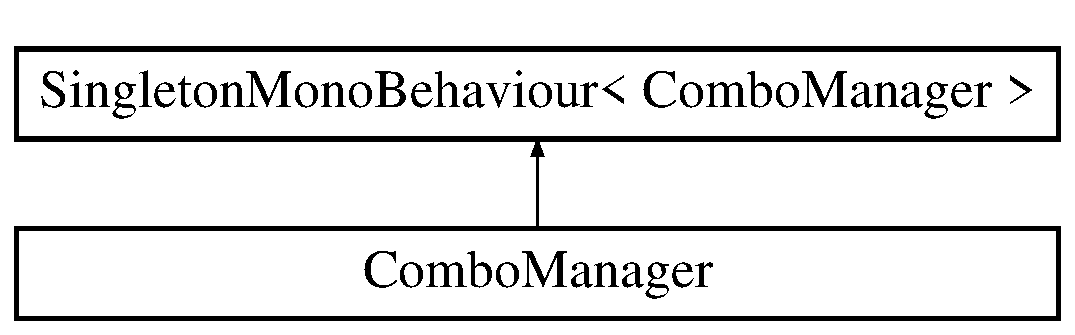
\includegraphics[height=2.000000cm]{class_combo_manager}
\end{center}
\end{figure}
\subsection*{Public Member Functions}
\begin{DoxyCompactItemize}
\item 
void \hyperlink{class_combo_manager_afcf63ba113ec108b6879cadfa6bc3be7}{Start\+Draw} (int combo)
\begin{DoxyCompactList}\small\item\em コンボ表示 \end{DoxyCompactList}\item 
void \hyperlink{class_combo_manager_a4c07555285dad869b35231f257f69db5}{Fail\+Combo} ()
\begin{DoxyCompactList}\small\item\em コンボ失敗時に非表示にする \end{DoxyCompactList}\end{DoxyCompactItemize}
\subsection*{Additional Inherited Members}


\subsection{Detailed Description}
コンボ管理クラス 



\subsection{Member Function Documentation}
\index{Combo\+Manager@{Combo\+Manager}!Fail\+Combo@{Fail\+Combo}}
\index{Fail\+Combo@{Fail\+Combo}!Combo\+Manager@{Combo\+Manager}}
\subsubsection[{\texorpdfstring{Fail\+Combo()}{FailCombo()}}]{\setlength{\rightskip}{0pt plus 5cm}void Combo\+Manager.\+Fail\+Combo (
\begin{DoxyParamCaption}
{}
\end{DoxyParamCaption}
)\hspace{0.3cm}{\ttfamily [inline]}}\hypertarget{class_combo_manager_a4c07555285dad869b35231f257f69db5}{}\label{class_combo_manager_a4c07555285dad869b35231f257f69db5}


コンボ失敗時に非表示にする 

\index{Combo\+Manager@{Combo\+Manager}!Start\+Draw@{Start\+Draw}}
\index{Start\+Draw@{Start\+Draw}!Combo\+Manager@{Combo\+Manager}}
\subsubsection[{\texorpdfstring{Start\+Draw(int combo)}{StartDraw(int combo)}}]{\setlength{\rightskip}{0pt plus 5cm}void Combo\+Manager.\+Start\+Draw (
\begin{DoxyParamCaption}
\item[{int}]{combo}
\end{DoxyParamCaption}
)\hspace{0.3cm}{\ttfamily [inline]}}\hypertarget{class_combo_manager_afcf63ba113ec108b6879cadfa6bc3be7}{}\label{class_combo_manager_afcf63ba113ec108b6879cadfa6bc3be7}


コンボ表示 


\begin{DoxyParams}{Parameters}
{\em combo} & \\
\hline
\end{DoxyParams}


The documentation for this class was generated from the following file\+:\begin{DoxyCompactItemize}
\item 
Scripts/\+Combo/Combo\+Manager.\+cs\end{DoxyCompactItemize}

\hypertarget{class_credit_contoroller}{}\section{Credit\+Contoroller Class Reference}
\label{class_credit_contoroller}\index{Credit\+Contoroller@{Credit\+Contoroller}}


クレジットシーンコントローラー  


Inheritance diagram for Credit\+Contoroller\+:\begin{figure}[H]
\begin{center}
\leavevmode
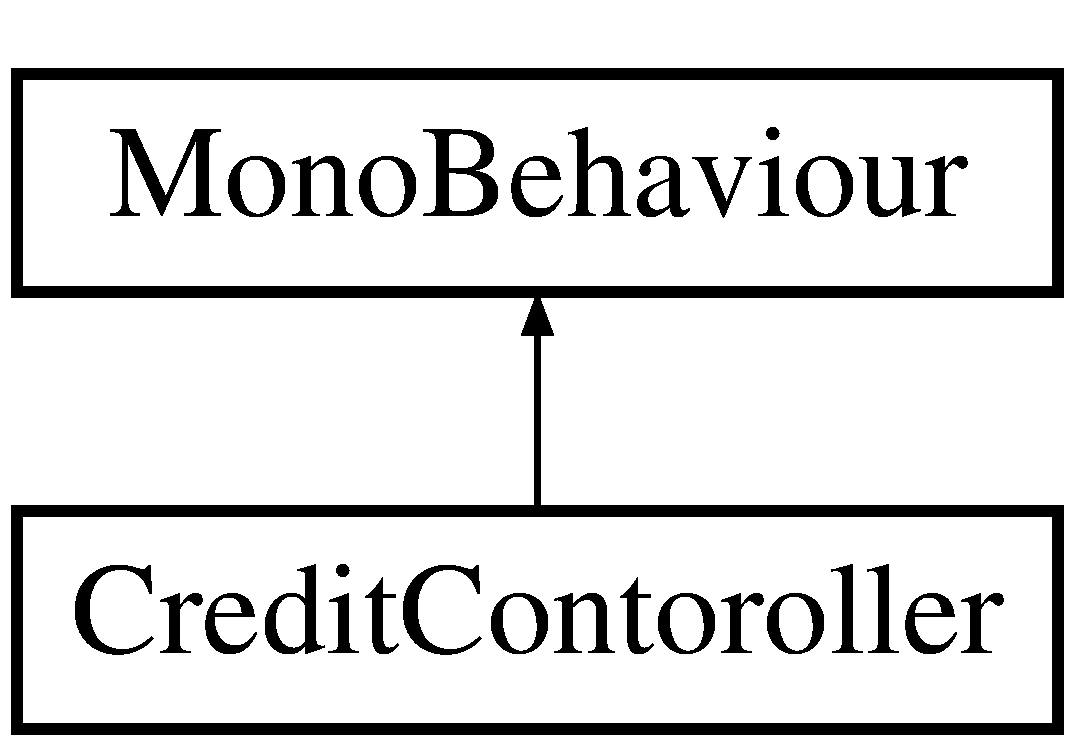
\includegraphics[height=2.000000cm]{class_credit_contoroller}
\end{center}
\end{figure}
\subsection*{Public Member Functions}
\begin{DoxyCompactItemize}
\item 
void \hyperlink{class_credit_contoroller_a325dd47e94a65f50e16a7868da731134}{Trans\+Title} ()
\begin{DoxyCompactList}\small\item\em タイトルに戻る \end{DoxyCompactList}\end{DoxyCompactItemize}


\subsection{Detailed Description}
クレジットシーンコントローラー 



\subsection{Member Function Documentation}
\index{Credit\+Contoroller@{Credit\+Contoroller}!Trans\+Title@{Trans\+Title}}
\index{Trans\+Title@{Trans\+Title}!Credit\+Contoroller@{Credit\+Contoroller}}
\subsubsection[{\texorpdfstring{Trans\+Title()}{TransTitle()}}]{\setlength{\rightskip}{0pt plus 5cm}void Credit\+Contoroller.\+Trans\+Title (
\begin{DoxyParamCaption}
{}
\end{DoxyParamCaption}
)\hspace{0.3cm}{\ttfamily [inline]}}\hypertarget{class_credit_contoroller_a325dd47e94a65f50e16a7868da731134}{}\label{class_credit_contoroller_a325dd47e94a65f50e16a7868da731134}


タイトルに戻る 



The documentation for this class was generated from the following file\+:\begin{DoxyCompactItemize}
\item 
Scripts/\+Scenes\+Controller/Credit\+Contoroller.\+cs\end{DoxyCompactItemize}

\hypertarget{class_entertainment_fire_works}{}\section{Entertainment\+Fire\+Works Class Reference}
\label{class_entertainment_fire_works}\index{Entertainment\+Fire\+Works@{Entertainment\+Fire\+Works}}


遊び心満載の花火打ち上げの制御  


Inheritance diagram for Entertainment\+Fire\+Works\+:\begin{figure}[H]
\begin{center}
\leavevmode
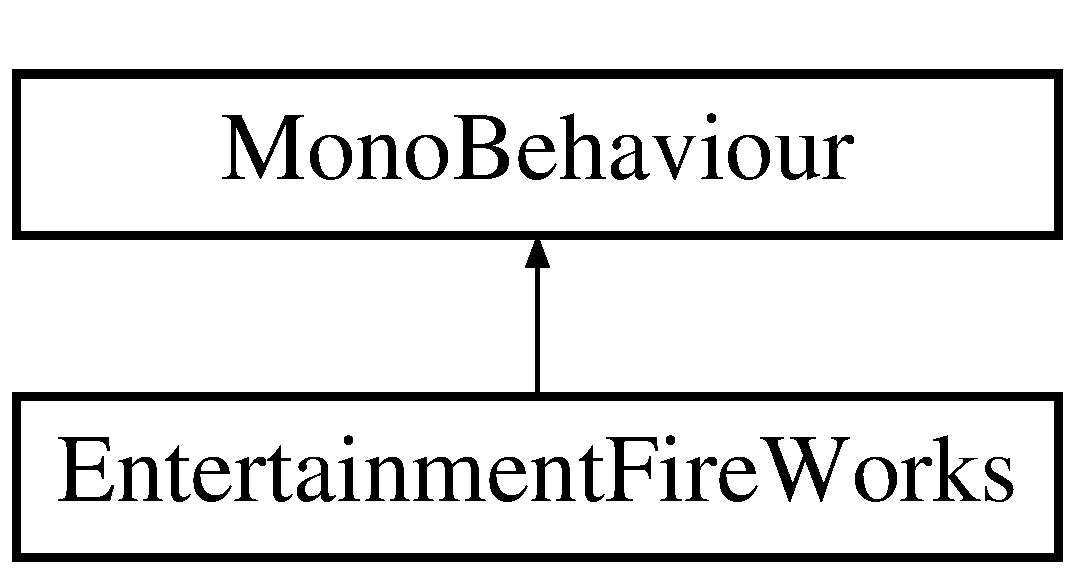
\includegraphics[height=2.000000cm]{class_entertainment_fire_works}
\end{center}
\end{figure}
\subsection*{Public Member Functions}
\begin{DoxyCompactItemize}
\item 
void \hyperlink{class_entertainment_fire_works_a5b3617d21d7a11d3661fa3d7816e6a72}{Launch\+Fire\+Works} ()
\begin{DoxyCompactList}\small\item\em 花火の打ち上げ \end{DoxyCompactList}\end{DoxyCompactItemize}


\subsection{Detailed Description}
遊び心満載の花火打ち上げの制御 



\subsection{Member Function Documentation}
\index{Entertainment\+Fire\+Works@{Entertainment\+Fire\+Works}!Launch\+Fire\+Works@{Launch\+Fire\+Works}}
\index{Launch\+Fire\+Works@{Launch\+Fire\+Works}!Entertainment\+Fire\+Works@{Entertainment\+Fire\+Works}}
\subsubsection[{\texorpdfstring{Launch\+Fire\+Works()}{LaunchFireWorks()}}]{\setlength{\rightskip}{0pt plus 5cm}void Entertainment\+Fire\+Works.\+Launch\+Fire\+Works (
\begin{DoxyParamCaption}
{}
\end{DoxyParamCaption}
)\hspace{0.3cm}{\ttfamily [inline]}}\hypertarget{class_entertainment_fire_works_a5b3617d21d7a11d3661fa3d7816e6a72}{}\label{class_entertainment_fire_works_a5b3617d21d7a11d3661fa3d7816e6a72}


花火の打ち上げ 



The documentation for this class was generated from the following file\+:\begin{DoxyCompactItemize}
\item 
Scripts/\+Entertainment/Entertainment\+Fire\+Works.\+cs\end{DoxyCompactItemize}

\hypertarget{class_entertainment_seeds_pool}{}\section{Entertainment\+Seeds\+Pool Class Reference}
\label{class_entertainment_seeds_pool}\index{Entertainment\+Seeds\+Pool@{Entertainment\+Seeds\+Pool}}


開演準備の花火打ち上げシード  


Inheritance diagram for Entertainment\+Seeds\+Pool\+:\begin{figure}[H]
\begin{center}
\leavevmode
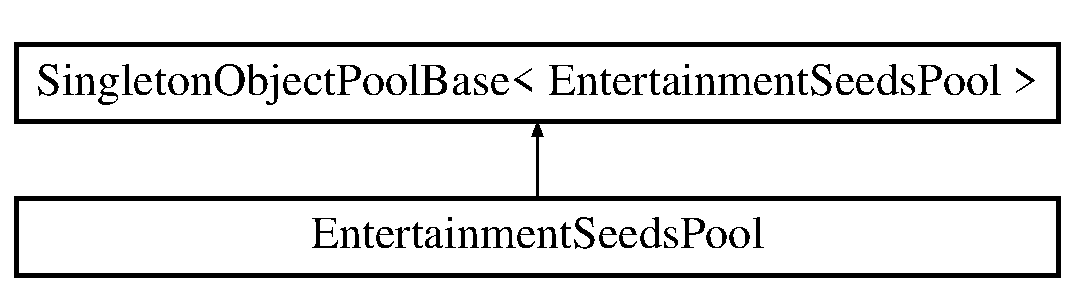
\includegraphics[height=2.000000cm]{class_entertainment_seeds_pool}
\end{center}
\end{figure}
\subsection*{Additional Inherited Members}


\subsection{Detailed Description}
開演準備の花火打ち上げシード 



The documentation for this class was generated from the following file\+:\begin{DoxyCompactItemize}
\item 
Scripts/\+Object\+Pool/Entertainment\+Seeds\+Pool.\+cs\end{DoxyCompactItemize}

\hypertarget{class_fail_tilte_logo}{}\section{Fail\+Tilte\+Logo Class Reference}
\label{class_fail_tilte_logo}\index{Fail\+Tilte\+Logo@{Fail\+Tilte\+Logo}}
Inheritance diagram for Fail\+Tilte\+Logo\+:\begin{figure}[H]
\begin{center}
\leavevmode
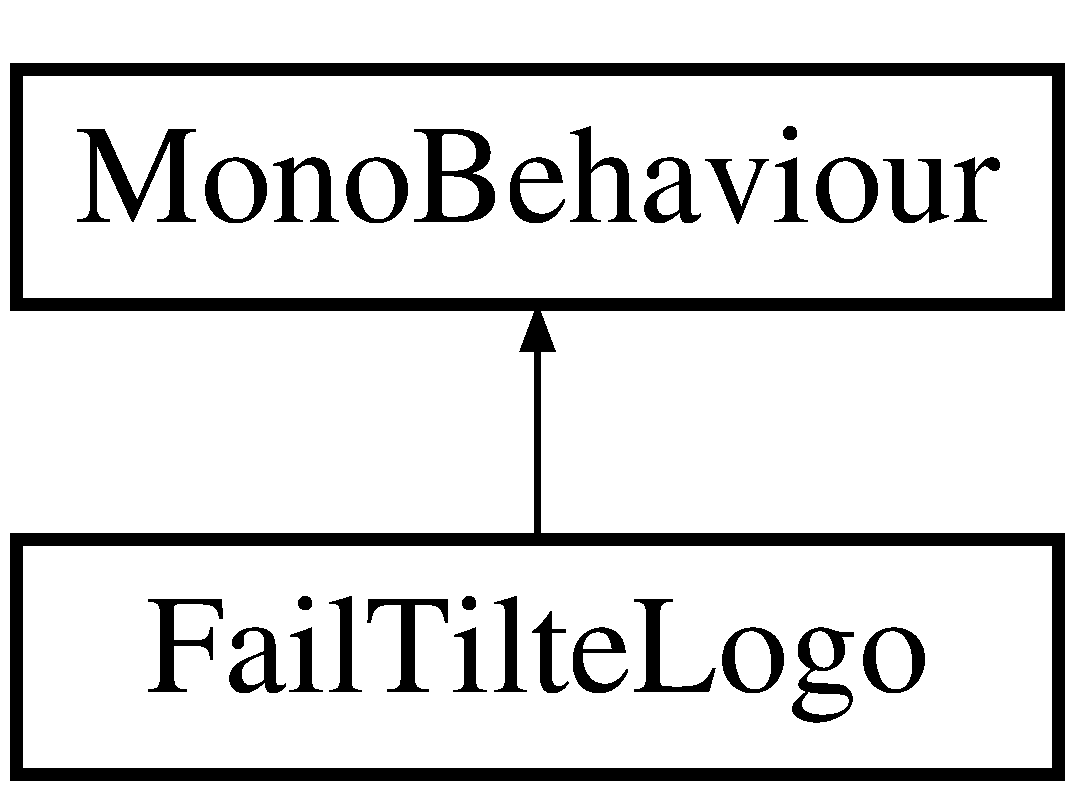
\includegraphics[height=2.000000cm]{class_fail_tilte_logo}
\end{center}
\end{figure}
\subsection*{Public Member Functions}
\begin{DoxyCompactItemize}
\item 
I\+Enumerator \hyperlink{class_fail_tilte_logo_a818ff0431bb8bff98c041c07e42b5a0c}{Fall} (System.\+Action action=null)
\begin{DoxyCompactList}\small\item\em タイトルロゴ \end{DoxyCompactList}\item 
void \hyperlink{class_fail_tilte_logo_a752af3aaff601fa6e79d6f281c9cf95f}{End\+Fall} ()
\begin{DoxyCompactList}\small\item\em 降下を一瞬で終わらせる \end{DoxyCompactList}\end{DoxyCompactItemize}


\subsection{Member Function Documentation}
\index{Fail\+Tilte\+Logo@{Fail\+Tilte\+Logo}!End\+Fall@{End\+Fall}}
\index{End\+Fall@{End\+Fall}!Fail\+Tilte\+Logo@{Fail\+Tilte\+Logo}}
\subsubsection[{\texorpdfstring{End\+Fall()}{EndFall()}}]{\setlength{\rightskip}{0pt plus 5cm}void Fail\+Tilte\+Logo.\+End\+Fall (
\begin{DoxyParamCaption}
{}
\end{DoxyParamCaption}
)\hspace{0.3cm}{\ttfamily [inline]}}\hypertarget{class_fail_tilte_logo_a752af3aaff601fa6e79d6f281c9cf95f}{}\label{class_fail_tilte_logo_a752af3aaff601fa6e79d6f281c9cf95f}


降下を一瞬で終わらせる 

\index{Fail\+Tilte\+Logo@{Fail\+Tilte\+Logo}!Fall@{Fall}}
\index{Fall@{Fall}!Fail\+Tilte\+Logo@{Fail\+Tilte\+Logo}}
\subsubsection[{\texorpdfstring{Fall(\+System.\+Action action=null)}{Fall(System.Action action=null)}}]{\setlength{\rightskip}{0pt plus 5cm}I\+Enumerator Fail\+Tilte\+Logo.\+Fall (
\begin{DoxyParamCaption}
\item[{System.\+Action}]{action = {\ttfamily null}}
\end{DoxyParamCaption}
)\hspace{0.3cm}{\ttfamily [inline]}}\hypertarget{class_fail_tilte_logo_a818ff0431bb8bff98c041c07e42b5a0c}{}\label{class_fail_tilte_logo_a818ff0431bb8bff98c041c07e42b5a0c}


タイトルロゴ 

\begin{DoxyReturn}{Returns}

\end{DoxyReturn}


The documentation for this class was generated from the following file\+:\begin{DoxyCompactItemize}
\item 
Scripts/\+U\+I/Fail\+Tilte\+Logo.\+cs\end{DoxyCompactItemize}

\hypertarget{class_file_manager}{}\section{File\+Manager Class Reference}
\label{class_file_manager}\index{File\+Manager@{File\+Manager}}
Inheritance diagram for File\+Manager\+:\begin{figure}[H]
\begin{center}
\leavevmode
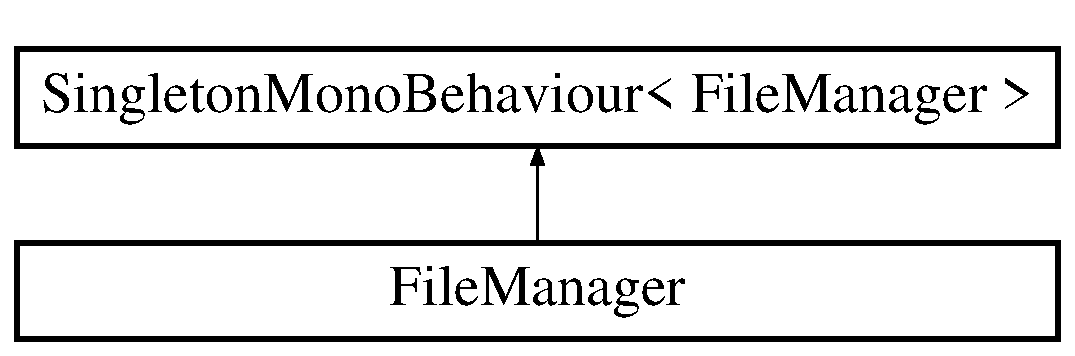
\includegraphics[height=2.000000cm]{class_file_manager}
\end{center}
\end{figure}
\subsection*{Public Member Functions}
\begin{DoxyCompactItemize}
\item 
I\+Enumerator {\bfseries Load} (string file\+Path, Action$<$ string $>$ data)\hypertarget{class_file_manager_a769410809bea75b7c9e8c6678b9742b3}{}\label{class_file_manager_a769410809bea75b7c9e8c6678b9742b3}

\item 
I\+Enumerator {\bfseries Read\+File} (string load\+Path)\hypertarget{class_file_manager_ab9ead949d5c94557a503910e75fea2f6}{}\label{class_file_manager_ab9ead949d5c94557a503910e75fea2f6}

\item 
I\+Enumerator \hyperlink{class_file_manager_a1df651a1bceee515bb1c4c77af2f5b23}{First\+Read\+File\+For\+Android} (string load\+Path)
\item 
I\+Enumerator {\bfseries Wait\+For\+Loading} ()\hypertarget{class_file_manager_ae05627d9f9a85fe0c7448c9430a00b72}{}\label{class_file_manager_ae05627d9f9a85fe0c7448c9430a00b72}

\item 
void {\bfseries Write} (string file\+Path, string contents, bool is\+Over\+Write=true)\hypertarget{class_file_manager_a4022cf7800e48d934b7c5fb47cd8bf06}{}\label{class_file_manager_a4022cf7800e48d934b7c5fb47cd8bf06}

\item 
void {\bfseries Delete} (string file\+Path)\hypertarget{class_file_manager_ac1fc354c1a1f90f4eb5b72baac6a6e39}{}\label{class_file_manager_ac1fc354c1a1f90f4eb5b72baac6a6e39}

\item 
bool {\bfseries Check\+File} (string file\+Path)\hypertarget{class_file_manager_a04b637c2ec7e4c0f0f28e6a99c72e138}{}\label{class_file_manager_a04b637c2ec7e4c0f0f28e6a99c72e138}

\end{DoxyCompactItemize}
\subsection*{Properties}
\begin{DoxyCompactItemize}
\item 
bool {\bfseries is\+Loading}\hspace{0.3cm}{\ttfamily  \mbox{[}get\mbox{]}}\hypertarget{class_file_manager_ab1d8ec56543ab3a376290848de4b13fc}{}\label{class_file_manager_ab1d8ec56543ab3a376290848de4b13fc}

\item 
static readonly string {\bfseries Streaming\+Assets\+Path}\hspace{0.3cm}{\ttfamily  \mbox{[}get\mbox{]}}\hypertarget{class_file_manager_a8c4d0b8139a34e420a5e37310490dab9}{}\label{class_file_manager_a8c4d0b8139a34e420a5e37310490dab9}

\end{DoxyCompactItemize}


\subsection{Member Function Documentation}
\index{File\+Manager@{File\+Manager}!First\+Read\+File\+For\+Android@{First\+Read\+File\+For\+Android}}
\index{First\+Read\+File\+For\+Android@{First\+Read\+File\+For\+Android}!File\+Manager@{File\+Manager}}
\subsubsection[{\texorpdfstring{First\+Read\+File\+For\+Android(string load\+Path)}{FirstReadFileForAndroid(string loadPath)}}]{\setlength{\rightskip}{0pt plus 5cm}I\+Enumerator File\+Manager.\+First\+Read\+File\+For\+Android (
\begin{DoxyParamCaption}
\item[{string}]{load\+Path}
\end{DoxyParamCaption}
)\hspace{0.3cm}{\ttfamily [inline]}}\hypertarget{class_file_manager_a1df651a1bceee515bb1c4c77af2f5b23}{}\label{class_file_manager_a1df651a1bceee515bb1c4c77af2f5b23}
wwwの通信が終わるまで待機 

The documentation for this class was generated from the following file\+:\begin{DoxyCompactItemize}
\item 
Scripts/\+File/File\+Manager.\+cs\end{DoxyCompactItemize}

\hypertarget{class_game_scene_controller}{}\section{Game\+Scene\+Controller Class Reference}
\label{class_game_scene_controller}\index{Game\+Scene\+Controller@{Game\+Scene\+Controller}}


ゲームシーンをコントロール  


Inheritance diagram for Game\+Scene\+Controller\+:\begin{figure}[H]
\begin{center}
\leavevmode
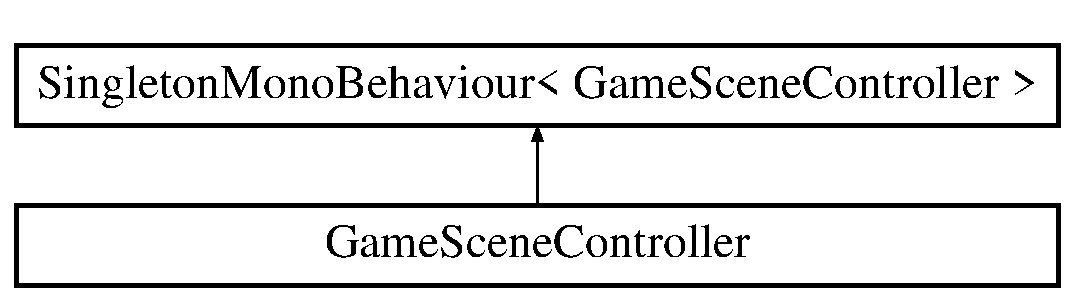
\includegraphics[height=2.000000cm]{class_game_scene_controller}
\end{center}
\end{figure}
\subsection*{Public Member Functions}
\begin{DoxyCompactItemize}
\item 
void \hyperlink{class_game_scene_controller_a011817ccbd771348e030649cda716168}{Set\+Pause} ()
\begin{DoxyCompactList}\small\item\em ポーズ処理 \end{DoxyCompactList}\item 
void \hyperlink{class_game_scene_controller_abdb3f81215251f33d62868fd089499c7}{Set\+Un\+Pause} ()
\begin{DoxyCompactList}\small\item\em ポーズ解除処理 \end{DoxyCompactList}\end{DoxyCompactItemize}
\subsection*{Public Attributes}
\begin{DoxyCompactItemize}
\item 
string {\bfseries file\+Path} = \char`\"{}/Music/0405.txt\char`\"{}\hypertarget{class_game_scene_controller_a7b2384e203698f395ed8e42ca79aaa4c}{}\label{class_game_scene_controller_a7b2384e203698f395ed8e42ca79aaa4c}

\end{DoxyCompactItemize}
\subsection*{Properties}
\begin{DoxyCompactItemize}
\item 
bool {\bfseries is\+Pause}\hspace{0.3cm}{\ttfamily  \mbox{[}get\mbox{]}}\hypertarget{class_game_scene_controller_a968a90d4bf02fb1f13349f951fd345ae}{}\label{class_game_scene_controller_a968a90d4bf02fb1f13349f951fd345ae}

\end{DoxyCompactItemize}


\subsection{Detailed Description}
ゲームシーンをコントロール 



\subsection{Member Function Documentation}
\index{Game\+Scene\+Controller@{Game\+Scene\+Controller}!Set\+Pause@{Set\+Pause}}
\index{Set\+Pause@{Set\+Pause}!Game\+Scene\+Controller@{Game\+Scene\+Controller}}
\subsubsection[{\texorpdfstring{Set\+Pause()}{SetPause()}}]{\setlength{\rightskip}{0pt plus 5cm}void Game\+Scene\+Controller.\+Set\+Pause (
\begin{DoxyParamCaption}
{}
\end{DoxyParamCaption}
)\hspace{0.3cm}{\ttfamily [inline]}}\hypertarget{class_game_scene_controller_a011817ccbd771348e030649cda716168}{}\label{class_game_scene_controller_a011817ccbd771348e030649cda716168}


ポーズ処理 

\index{Game\+Scene\+Controller@{Game\+Scene\+Controller}!Set\+Un\+Pause@{Set\+Un\+Pause}}
\index{Set\+Un\+Pause@{Set\+Un\+Pause}!Game\+Scene\+Controller@{Game\+Scene\+Controller}}
\subsubsection[{\texorpdfstring{Set\+Un\+Pause()}{SetUnPause()}}]{\setlength{\rightskip}{0pt plus 5cm}void Game\+Scene\+Controller.\+Set\+Un\+Pause (
\begin{DoxyParamCaption}
{}
\end{DoxyParamCaption}
)\hspace{0.3cm}{\ttfamily [inline]}}\hypertarget{class_game_scene_controller_abdb3f81215251f33d62868fd089499c7}{}\label{class_game_scene_controller_abdb3f81215251f33d62868fd089499c7}


ポーズ解除処理 



The documentation for this class was generated from the following file\+:\begin{DoxyCompactItemize}
\item 
Scripts/\+Scenes\+Controller/Game\+Scene\+Controller.\+cs\end{DoxyCompactItemize}

\hypertarget{class_judge_manager}{}\section{Judge\+Manager Class Reference}
\label{class_judge_manager}\index{Judge\+Manager@{Judge\+Manager}}
Inheritance diagram for Judge\+Manager\+:\begin{figure}[H]
\begin{center}
\leavevmode
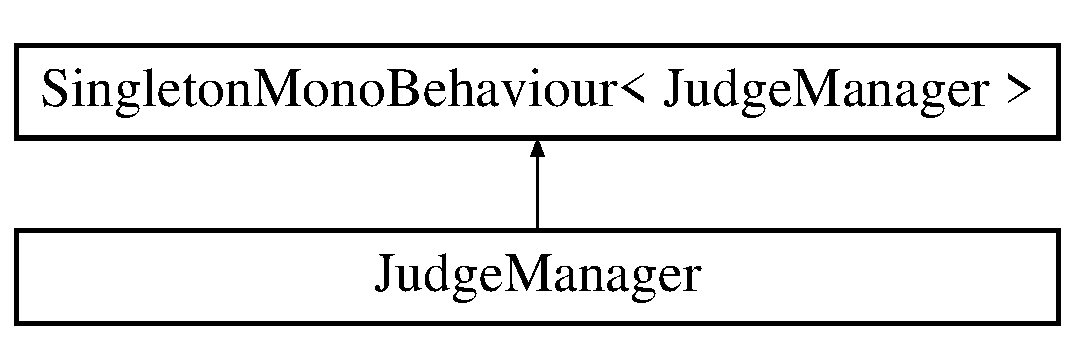
\includegraphics[height=2.000000cm]{class_judge_manager}
\end{center}
\end{figure}
\subsection*{Public Member Functions}
\begin{DoxyCompactItemize}
\item 
void {\bfseries Bad\+Score} ()\hypertarget{class_judge_manager_a12ab1b4163a77c8576af6a624f914a88}{}\label{class_judge_manager_a12ab1b4163a77c8576af6a624f914a88}

\item 
void {\bfseries Great\+Score} ()\hypertarget{class_judge_manager_a714edcdb57505441801355cefcdfb2b2}{}\label{class_judge_manager_a714edcdb57505441801355cefcdfb2b2}

\item 
void {\bfseries Perfect\+Score} ()\hypertarget{class_judge_manager_a9922beeef09f3808b6941c4a09653b60}{}\label{class_judge_manager_a9922beeef09f3808b6941c4a09653b60}

\end{DoxyCompactItemize}
\subsection*{Additional Inherited Members}


The documentation for this class was generated from the following file\+:\begin{DoxyCompactItemize}
\item 
Scripts/\+Judge/Judge\+Manager.\+cs\end{DoxyCompactItemize}

\hypertarget{class_serialize_1_1_key_and_value}{}\section{Serialize.\+Key\+And\+Value$<$ T\+Key, T\+Value $>$ Class Template Reference}
\label{class_serialize_1_1_key_and_value}\index{Serialize.\+Key\+And\+Value$<$ T\+Key, T\+Value $>$@{Serialize.\+Key\+And\+Value$<$ T\+Key, T\+Value $>$}}


シリアル化して視覚化するテーブルの要素(キーと値)  


\subsection*{Public Member Functions}
\begin{DoxyCompactItemize}
\item 
\hyperlink{class_serialize_1_1_key_and_value_a6455331fc8ad322e913a27a7aefcc1b4}{Key\+And\+Value} (T\+Key key, T\+Value value)
\begin{DoxyCompactList}\small\item\em 空コンストラクタ \end{DoxyCompactList}\item 
\hyperlink{class_serialize_1_1_key_and_value_a4a917a400efd3c0eda67eab00b4a7160}{Key\+And\+Value} (\hyperlink{class_serialize_1_1_key_and_value}{Key\+And\+Value}$<$ T\+Key, T\+Value $>$ pair)
\begin{DoxyCompactList}\small\item\em コンストラクタ \end{DoxyCompactList}\end{DoxyCompactItemize}
\subsection*{Public Attributes}
\begin{DoxyCompactItemize}
\item 
T\+Key {\bfseries key}\hypertarget{class_serialize_1_1_key_and_value_a09070d1ab43775ff20bb3c90b305b360}{}\label{class_serialize_1_1_key_and_value_a09070d1ab43775ff20bb3c90b305b360}

\item 
T\+Value {\bfseries value}\hypertarget{class_serialize_1_1_key_and_value_a64c9a11f4b75cbc6ef8d9c184b9f9813}{}\label{class_serialize_1_1_key_and_value_a64c9a11f4b75cbc6ef8d9c184b9f9813}

\end{DoxyCompactItemize}


\subsection{Detailed Description}
シリアル化して視覚化するテーブルの要素(キーと値) 


\begin{DoxyTemplParams}{Template Parameters}
{\em T\+Key} & \\
\hline
{\em T\+Value} & \\
\hline
\end{DoxyTemplParams}


\subsection{Constructor \& Destructor Documentation}
\index{Serialize\+::\+Key\+And\+Value@{Serialize\+::\+Key\+And\+Value}!Key\+And\+Value@{Key\+And\+Value}}
\index{Key\+And\+Value@{Key\+And\+Value}!Serialize\+::\+Key\+And\+Value@{Serialize\+::\+Key\+And\+Value}}
\subsubsection[{\texorpdfstring{Key\+And\+Value(\+T\+Key key, T\+Value value)}{KeyAndValue(TKey key, TValue value)}}]{\setlength{\rightskip}{0pt plus 5cm}{\bf Serialize.\+Key\+And\+Value}$<$ T\+Key, T\+Value $>$.{\bf Key\+And\+Value} (
\begin{DoxyParamCaption}
\item[{T\+Key}]{key, }
\item[{T\+Value}]{value}
\end{DoxyParamCaption}
)\hspace{0.3cm}{\ttfamily [inline]}}\hypertarget{class_serialize_1_1_key_and_value_a6455331fc8ad322e913a27a7aefcc1b4}{}\label{class_serialize_1_1_key_and_value_a6455331fc8ad322e913a27a7aefcc1b4}


空コンストラクタ 

コンストラクタ 


\begin{DoxyParams}{Parameters}
{\em key} & 登録キー\\
\hline
{\em value} & 登録値\\
\hline
\end{DoxyParams}
\index{Serialize\+::\+Key\+And\+Value@{Serialize\+::\+Key\+And\+Value}!Key\+And\+Value@{Key\+And\+Value}}
\index{Key\+And\+Value@{Key\+And\+Value}!Serialize\+::\+Key\+And\+Value@{Serialize\+::\+Key\+And\+Value}}
\subsubsection[{\texorpdfstring{Key\+And\+Value(\+Key\+And\+Value$<$ T\+Key, T\+Value $>$ pair)}{KeyAndValue(KeyAndValue< TKey, TValue > pair)}}]{\setlength{\rightskip}{0pt plus 5cm}{\bf Serialize.\+Key\+And\+Value}$<$ T\+Key, T\+Value $>$.{\bf Key\+And\+Value} (
\begin{DoxyParamCaption}
\item[{{\bf Key\+And\+Value}$<$ T\+Key, T\+Value $>$}]{pair}
\end{DoxyParamCaption}
)\hspace{0.3cm}{\ttfamily [inline]}}\hypertarget{class_serialize_1_1_key_and_value_a4a917a400efd3c0eda67eab00b4a7160}{}\label{class_serialize_1_1_key_and_value_a4a917a400efd3c0eda67eab00b4a7160}


コンストラクタ 


\begin{DoxyParams}{Parameters}
{\em pair} & 登録するペア\\
\hline
\end{DoxyParams}


The documentation for this class was generated from the following file\+:\begin{DoxyCompactItemize}
\item 
Scripts/\+Base/Table\+Base.\+cs\end{DoxyCompactItemize}

\hypertarget{class_lane}{}\section{Lane Class Reference}
\label{class_lane}\index{Lane@{Lane}}


レーン  


Inheritance diagram for Lane\+:\begin{figure}[H]
\begin{center}
\leavevmode
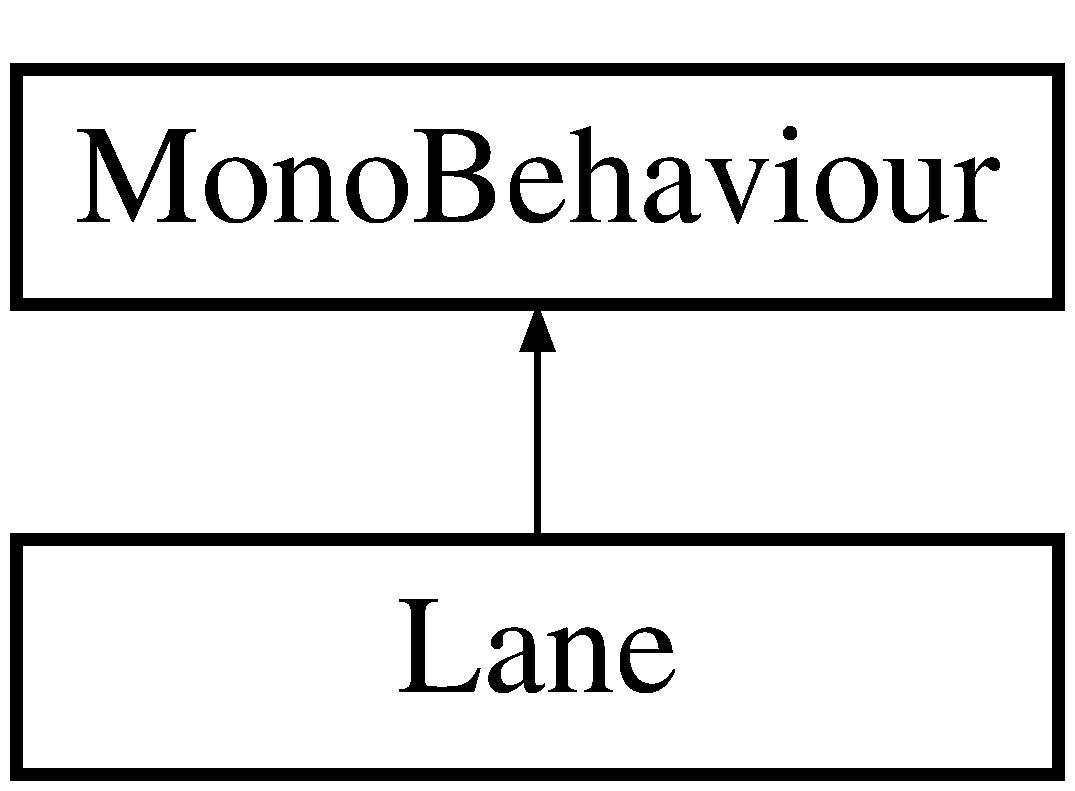
\includegraphics[height=2.000000cm]{class_lane}
\end{center}
\end{figure}
\subsection*{Public Member Functions}
\begin{DoxyCompactItemize}
\item 
void {\bfseries update} ()\hypertarget{class_lane_ab114e90cdab138167d959014930c7e14}{}\label{class_lane_ab114e90cdab138167d959014930c7e14}

\item 
void \hyperlink{class_lane_af823b917f0b54ccc138815a8bd25e773}{Init} ()
\begin{DoxyCompactList}\small\item\em 初期化 \end{DoxyCompactList}\end{DoxyCompactItemize}
\subsection*{Properties}
\begin{DoxyCompactItemize}
\item 
Vector3 {\bfseries Tap\+Point\+Center}\hspace{0.3cm}{\ttfamily  \mbox{[}get\mbox{]}}\hypertarget{class_lane_a290e3d76fff1549f54065187e42a0c0e}{}\label{class_lane_a290e3d76fff1549f54065187e42a0c0e}

\end{DoxyCompactItemize}


\subsection{Detailed Description}
レーン 



\subsection{Member Function Documentation}
\index{Lane@{Lane}!Init@{Init}}
\index{Init@{Init}!Lane@{Lane}}
\subsubsection[{\texorpdfstring{Init()}{Init()}}]{\setlength{\rightskip}{0pt plus 5cm}void Lane.\+Init (
\begin{DoxyParamCaption}
{}
\end{DoxyParamCaption}
)\hspace{0.3cm}{\ttfamily [inline]}}\hypertarget{class_lane_af823b917f0b54ccc138815a8bd25e773}{}\label{class_lane_af823b917f0b54ccc138815a8bd25e773}


初期化 



The documentation for this class was generated from the following file\+:\begin{DoxyCompactItemize}
\item 
Scripts/\+Lane/Lane.\+cs\end{DoxyCompactItemize}

\hypertarget{class_lane_manager}{}\section{Lane\+Manager Class Reference}
\label{class_lane_manager}\index{Lane\+Manager@{Lane\+Manager}}
Inheritance diagram for Lane\+Manager\+:\begin{figure}[H]
\begin{center}
\leavevmode
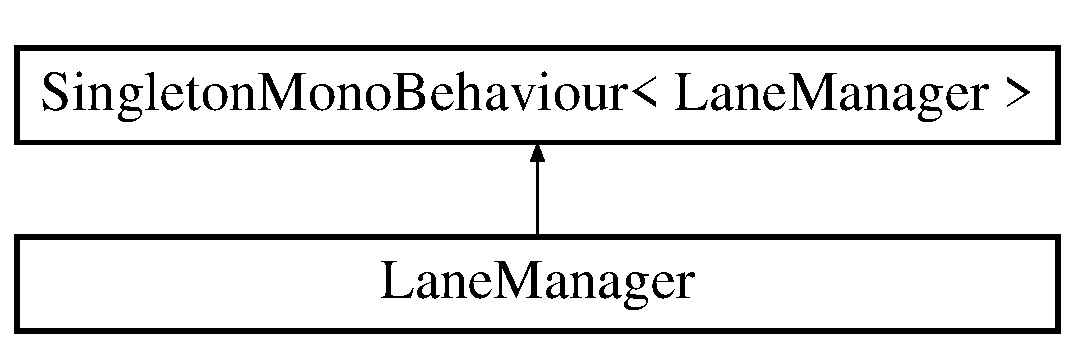
\includegraphics[height=2.000000cm]{class_lane_manager}
\end{center}
\end{figure}
\subsection*{Public Member Functions}
\begin{DoxyCompactItemize}
\item 
void \hyperlink{class_lane_manager_acc5a0b76fee2459a9c5af08554f8dfc4}{Init} ()
\begin{DoxyCompactList}\small\item\em 初期化 \end{DoxyCompactList}\item 
void \hyperlink{class_lane_manager_a7b5a2327aaf8750abc07ecddbeecd431}{update} ()
\begin{DoxyCompactList}\small\item\em 更新 \end{DoxyCompactList}\item 
Vector3 {\bfseries Get\+Lane\+Tap\+Point\+Center} (int lane\+No)\hypertarget{class_lane_manager_a10cd73d620e3892b9572575afaf88103}{}\label{class_lane_manager_a10cd73d620e3892b9572575afaf88103}

\item 
int \hyperlink{class_lane_manager_a7f183791322e811b1021b19f77c3d98b}{Get\+Lane\+No} (Vector3 pos)
\begin{DoxyCompactList}\small\item\em 座標からレーン番号を取得 \end{DoxyCompactList}\item 
Game\+Object {\bfseries Get\+Mask\+Object} (int lane\+No)\hypertarget{class_lane_manager_aa7c8fa846e3f027cd7d585a96746e3a3}{}\label{class_lane_manager_aa7c8fa846e3f027cd7d585a96746e3a3}

\end{DoxyCompactItemize}
\subsection*{Additional Inherited Members}


\subsection{Member Function Documentation}
\index{Lane\+Manager@{Lane\+Manager}!Get\+Lane\+No@{Get\+Lane\+No}}
\index{Get\+Lane\+No@{Get\+Lane\+No}!Lane\+Manager@{Lane\+Manager}}
\subsubsection[{\texorpdfstring{Get\+Lane\+No(\+Vector3 pos)}{GetLaneNo(Vector3 pos)}}]{\setlength{\rightskip}{0pt plus 5cm}int Lane\+Manager.\+Get\+Lane\+No (
\begin{DoxyParamCaption}
\item[{Vector3}]{pos}
\end{DoxyParamCaption}
)\hspace{0.3cm}{\ttfamily [inline]}}\hypertarget{class_lane_manager_a7f183791322e811b1021b19f77c3d98b}{}\label{class_lane_manager_a7f183791322e811b1021b19f77c3d98b}


座標からレーン番号を取得 


\begin{DoxyParams}{Parameters}
{\em pos} & \\
\hline
\end{DoxyParams}
\begin{DoxyReturn}{Returns}

\end{DoxyReturn}
\index{Lane\+Manager@{Lane\+Manager}!Init@{Init}}
\index{Init@{Init}!Lane\+Manager@{Lane\+Manager}}
\subsubsection[{\texorpdfstring{Init()}{Init()}}]{\setlength{\rightskip}{0pt plus 5cm}void Lane\+Manager.\+Init (
\begin{DoxyParamCaption}
{}
\end{DoxyParamCaption}
)\hspace{0.3cm}{\ttfamily [inline]}}\hypertarget{class_lane_manager_acc5a0b76fee2459a9c5af08554f8dfc4}{}\label{class_lane_manager_acc5a0b76fee2459a9c5af08554f8dfc4}


初期化 

\index{Lane\+Manager@{Lane\+Manager}!update@{update}}
\index{update@{update}!Lane\+Manager@{Lane\+Manager}}
\subsubsection[{\texorpdfstring{update()}{update()}}]{\setlength{\rightskip}{0pt plus 5cm}void Lane\+Manager.\+update (
\begin{DoxyParamCaption}
{}
\end{DoxyParamCaption}
)\hspace{0.3cm}{\ttfamily [inline]}}\hypertarget{class_lane_manager_a7b5a2327aaf8750abc07ecddbeecd431}{}\label{class_lane_manager_a7b5a2327aaf8750abc07ecddbeecd431}


更新 



The documentation for this class was generated from the following file\+:\begin{DoxyCompactItemize}
\item 
Scripts/\+Lane/Lane\+Manager.\+cs\end{DoxyCompactItemize}

\hypertarget{class_long_notes}{}\section{Long\+Notes Class Reference}
\label{class_long_notes}\index{Long\+Notes@{Long\+Notes}}


長押しノーツ  


Inheritance diagram for Long\+Notes\+:\begin{figure}[H]
\begin{center}
\leavevmode
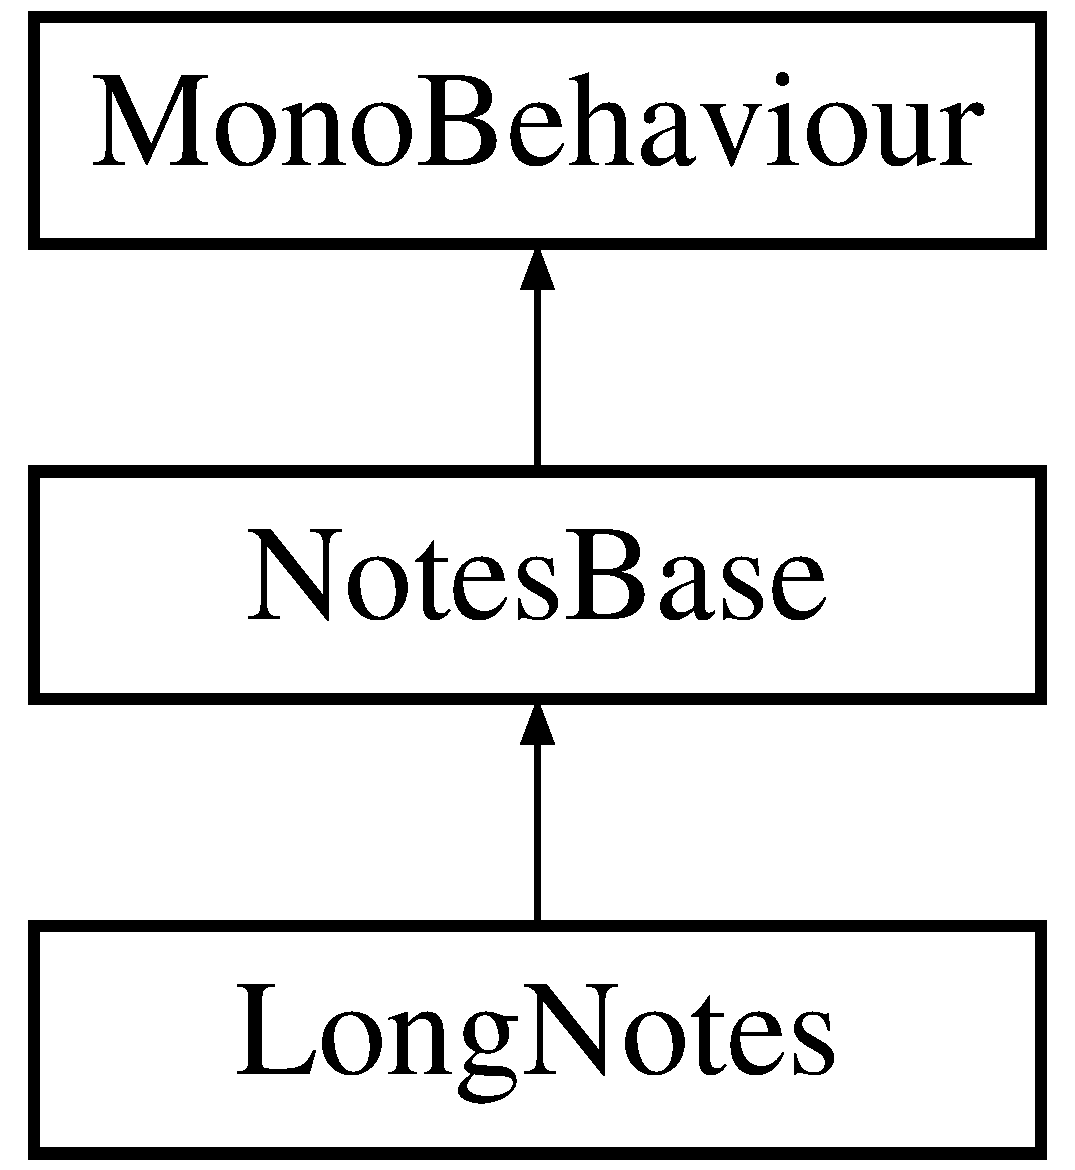
\includegraphics[height=3.000000cm]{class_long_notes}
\end{center}
\end{figure}
\subsection*{Public Member Functions}
\begin{DoxyCompactItemize}
\item 
override void \hyperlink{class_long_notes_a080003953680dc4bfa81ef19cabae1c7}{Init} (int lane\+No, float down, float up)
\begin{DoxyCompactList}\small\item\em 初期化 \end{DoxyCompactList}\item 
override void \hyperlink{class_long_notes_a8af8f2d9bd19746a903571ddbde988d9}{Move} ()
\begin{DoxyCompactList}\small\item\em 移動 \end{DoxyCompactList}\item 
void \hyperlink{class_long_notes_a7f87f264cfd9cc1eb4d5eaa48a1c0be2}{On\+Touch\+Began} ()
\begin{DoxyCompactList}\small\item\em 押したときの処理 \end{DoxyCompactList}\item 
void \hyperlink{class_long_notes_a33503ed24d2d1b642424f0c106c5d8e3}{On\+Touch\+End} ()
\begin{DoxyCompactList}\small\item\em タッチが離された時の処理 \end{DoxyCompactList}\item 
override void \hyperlink{class_long_notes_acebb95804b8bb34b709d74b4d97518dd}{Miss} ()
\begin{DoxyCompactList}\small\item\em 失敗処理 \end{DoxyCompactList}\item 
override void \hyperlink{class_long_notes_aefca60d75a0c00f72028f4656400e1d0}{Rec\+Init} (int lane\+No, float down, float up)
\begin{DoxyCompactList}\small\item\em 録画シーンの初期化 \end{DoxyCompactList}\end{DoxyCompactItemize}
\subsection*{Public Attributes}
\begin{DoxyCompactItemize}
\item 
const int {\bfseries ID} = 2\hypertarget{class_long_notes_a9669e9d0f3262d47000660258fbf3dd0}{}\label{class_long_notes_a9669e9d0f3262d47000660258fbf3dd0}

\end{DoxyCompactItemize}
\subsection*{Properties}
\begin{DoxyCompactItemize}
\item 
override bool \hyperlink{class_long_notes_a958688f3d3eaca0f9fffaa3fab9b6fd8}{is\+Reset}\hspace{0.3cm}{\ttfamily  \mbox{[}get\mbox{]}}
\begin{DoxyCompactList}\small\item\em リセットフラグ \end{DoxyCompactList}\item 
override bool \hyperlink{class_long_notes_aff79ae0d453a14c68ce63bf57c01c6b0}{is\+Miss}\hspace{0.3cm}{\ttfamily  \mbox{[}get\mbox{]}}
\begin{DoxyCompactList}\small\item\em ミスフラグ \end{DoxyCompactList}\end{DoxyCompactItemize}
\subsection*{Additional Inherited Members}


\subsection{Detailed Description}
長押しノーツ 



\subsection{Member Function Documentation}
\index{Long\+Notes@{Long\+Notes}!Init@{Init}}
\index{Init@{Init}!Long\+Notes@{Long\+Notes}}
\subsubsection[{\texorpdfstring{Init(int lane\+No, float down, float up)}{Init(int laneNo, float down, float up)}}]{\setlength{\rightskip}{0pt plus 5cm}override void Long\+Notes.\+Init (
\begin{DoxyParamCaption}
\item[{int}]{lane\+No, }
\item[{float}]{down, }
\item[{float}]{up}
\end{DoxyParamCaption}
)\hspace{0.3cm}{\ttfamily [inline]}, {\ttfamily [virtual]}}\hypertarget{class_long_notes_a080003953680dc4bfa81ef19cabae1c7}{}\label{class_long_notes_a080003953680dc4bfa81ef19cabae1c7}


初期化 


\begin{DoxyParams}{Parameters}
{\em lane\+No} & \\
\hline
{\em down} & \\
\hline
{\em up} & \\
\hline
\end{DoxyParams}


Reimplemented from \hyperlink{class_notes_base}{Notes\+Base}.

\index{Long\+Notes@{Long\+Notes}!Miss@{Miss}}
\index{Miss@{Miss}!Long\+Notes@{Long\+Notes}}
\subsubsection[{\texorpdfstring{Miss()}{Miss()}}]{\setlength{\rightskip}{0pt plus 5cm}override void Long\+Notes.\+Miss (
\begin{DoxyParamCaption}
{}
\end{DoxyParamCaption}
)\hspace{0.3cm}{\ttfamily [inline]}, {\ttfamily [virtual]}}\hypertarget{class_long_notes_acebb95804b8bb34b709d74b4d97518dd}{}\label{class_long_notes_acebb95804b8bb34b709d74b4d97518dd}


失敗処理 



Reimplemented from \hyperlink{class_notes_base}{Notes\+Base}.

\index{Long\+Notes@{Long\+Notes}!Move@{Move}}
\index{Move@{Move}!Long\+Notes@{Long\+Notes}}
\subsubsection[{\texorpdfstring{Move()}{Move()}}]{\setlength{\rightskip}{0pt plus 5cm}override void Long\+Notes.\+Move (
\begin{DoxyParamCaption}
{}
\end{DoxyParamCaption}
)\hspace{0.3cm}{\ttfamily [inline]}, {\ttfamily [virtual]}}\hypertarget{class_long_notes_a8af8f2d9bd19746a903571ddbde988d9}{}\label{class_long_notes_a8af8f2d9bd19746a903571ddbde988d9}


移動 



Reimplemented from \hyperlink{class_notes_base}{Notes\+Base}.

\index{Long\+Notes@{Long\+Notes}!On\+Touch\+Began@{On\+Touch\+Began}}
\index{On\+Touch\+Began@{On\+Touch\+Began}!Long\+Notes@{Long\+Notes}}
\subsubsection[{\texorpdfstring{On\+Touch\+Began()}{OnTouchBegan()}}]{\setlength{\rightskip}{0pt plus 5cm}void Long\+Notes.\+On\+Touch\+Began (
\begin{DoxyParamCaption}
{}
\end{DoxyParamCaption}
)\hspace{0.3cm}{\ttfamily [inline]}}\hypertarget{class_long_notes_a7f87f264cfd9cc1eb4d5eaa48a1c0be2}{}\label{class_long_notes_a7f87f264cfd9cc1eb4d5eaa48a1c0be2}


押したときの処理 

\index{Long\+Notes@{Long\+Notes}!On\+Touch\+End@{On\+Touch\+End}}
\index{On\+Touch\+End@{On\+Touch\+End}!Long\+Notes@{Long\+Notes}}
\subsubsection[{\texorpdfstring{On\+Touch\+End()}{OnTouchEnd()}}]{\setlength{\rightskip}{0pt plus 5cm}void Long\+Notes.\+On\+Touch\+End (
\begin{DoxyParamCaption}
{}
\end{DoxyParamCaption}
)\hspace{0.3cm}{\ttfamily [inline]}}\hypertarget{class_long_notes_a33503ed24d2d1b642424f0c106c5d8e3}{}\label{class_long_notes_a33503ed24d2d1b642424f0c106c5d8e3}


タッチが離された時の処理 

\index{Long\+Notes@{Long\+Notes}!Rec\+Init@{Rec\+Init}}
\index{Rec\+Init@{Rec\+Init}!Long\+Notes@{Long\+Notes}}
\subsubsection[{\texorpdfstring{Rec\+Init(int lane\+No, float down, float up)}{RecInit(int laneNo, float down, float up)}}]{\setlength{\rightskip}{0pt plus 5cm}override void Long\+Notes.\+Rec\+Init (
\begin{DoxyParamCaption}
\item[{int}]{lane\+No, }
\item[{float}]{down, }
\item[{float}]{up}
\end{DoxyParamCaption}
)\hspace{0.3cm}{\ttfamily [inline]}, {\ttfamily [virtual]}}\hypertarget{class_long_notes_aefca60d75a0c00f72028f4656400e1d0}{}\label{class_long_notes_aefca60d75a0c00f72028f4656400e1d0}


録画シーンの初期化 



Reimplemented from \hyperlink{class_notes_base}{Notes\+Base}.



\subsection{Property Documentation}
\index{Long\+Notes@{Long\+Notes}!is\+Miss@{is\+Miss}}
\index{is\+Miss@{is\+Miss}!Long\+Notes@{Long\+Notes}}
\subsubsection[{\texorpdfstring{is\+Miss}{isMiss}}]{\setlength{\rightskip}{0pt plus 5cm}override bool Long\+Notes.\+is\+Miss\hspace{0.3cm}{\ttfamily [get]}}\hypertarget{class_long_notes_aff79ae0d453a14c68ce63bf57c01c6b0}{}\label{class_long_notes_aff79ae0d453a14c68ce63bf57c01c6b0}


ミスフラグ 

\index{Long\+Notes@{Long\+Notes}!is\+Reset@{is\+Reset}}
\index{is\+Reset@{is\+Reset}!Long\+Notes@{Long\+Notes}}
\subsubsection[{\texorpdfstring{is\+Reset}{isReset}}]{\setlength{\rightskip}{0pt plus 5cm}override bool Long\+Notes.\+is\+Reset\hspace{0.3cm}{\ttfamily [get]}}\hypertarget{class_long_notes_a958688f3d3eaca0f9fffaa3fab9b6fd8}{}\label{class_long_notes_a958688f3d3eaca0f9fffaa3fab9b6fd8}


リセットフラグ 



The documentation for this class was generated from the following file\+:\begin{DoxyCompactItemize}
\item 
Scripts/\+Notes/Long\+Notes.\+cs\end{DoxyCompactItemize}

\hypertarget{class_long_notes_big_fire_works}{}\section{Long\+Notes\+Big\+Fire\+Works Class Reference}
\label{class_long_notes_big_fire_works}\index{Long\+Notes\+Big\+Fire\+Works@{Long\+Notes\+Big\+Fire\+Works}}
Inheritance diagram for Long\+Notes\+Big\+Fire\+Works\+:\begin{figure}[H]
\begin{center}
\leavevmode
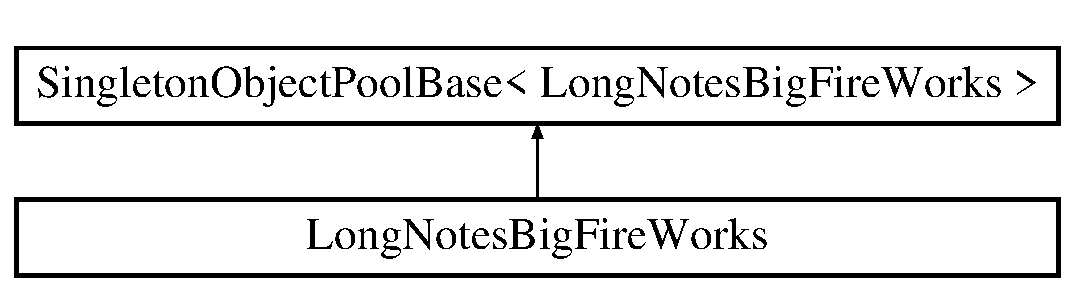
\includegraphics[height=2.000000cm]{class_long_notes_big_fire_works}
\end{center}
\end{figure}
\subsection*{Public Member Functions}
\begin{DoxyCompactItemize}
\item 
void {\bfseries Run} (Vector3 pos)\hypertarget{class_long_notes_big_fire_works_adb1c632ae5247e45829a7947626995e1}{}\label{class_long_notes_big_fire_works_adb1c632ae5247e45829a7947626995e1}

\end{DoxyCompactItemize}
\subsection*{Additional Inherited Members}


The documentation for this class was generated from the following file\+:\begin{DoxyCompactItemize}
\item 
Scripts/\+Object\+Pool/Long\+Notes\+Big\+Fire\+Works.\+cs\end{DoxyCompactItemize}

\hypertarget{class_long_notes_pool}{}\section{Long\+Notes\+Pool Class Reference}
\label{class_long_notes_pool}\index{Long\+Notes\+Pool@{Long\+Notes\+Pool}}
Inheritance diagram for Long\+Notes\+Pool\+:\begin{figure}[H]
\begin{center}
\leavevmode
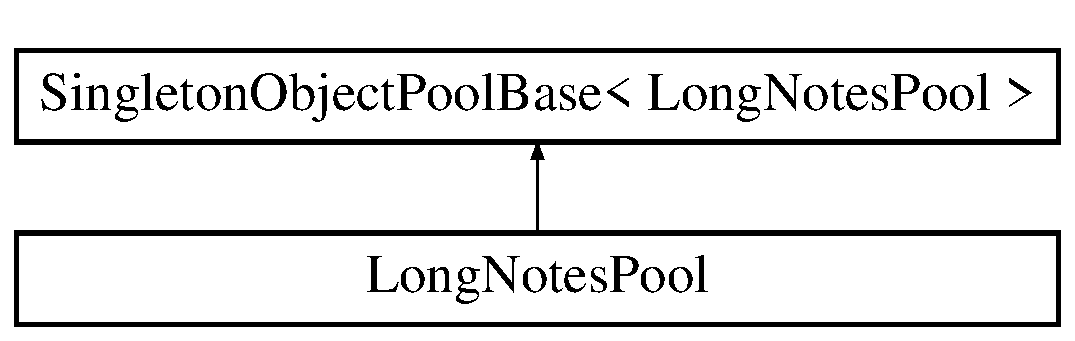
\includegraphics[height=2.000000cm]{class_long_notes_pool}
\end{center}
\end{figure}
\subsection*{Additional Inherited Members}


The documentation for this class was generated from the following file\+:\begin{DoxyCompactItemize}
\item 
Scripts/\+Object\+Pool/Long\+Notes\+Pool.\+cs\end{DoxyCompactItemize}

\hypertarget{class_long_notes_small_fire_works_pool}{}\section{Long\+Notes\+Small\+Fire\+Works\+Pool Class Reference}
\label{class_long_notes_small_fire_works_pool}\index{Long\+Notes\+Small\+Fire\+Works\+Pool@{Long\+Notes\+Small\+Fire\+Works\+Pool}}
Inheritance diagram for Long\+Notes\+Small\+Fire\+Works\+Pool\+:\begin{figure}[H]
\begin{center}
\leavevmode
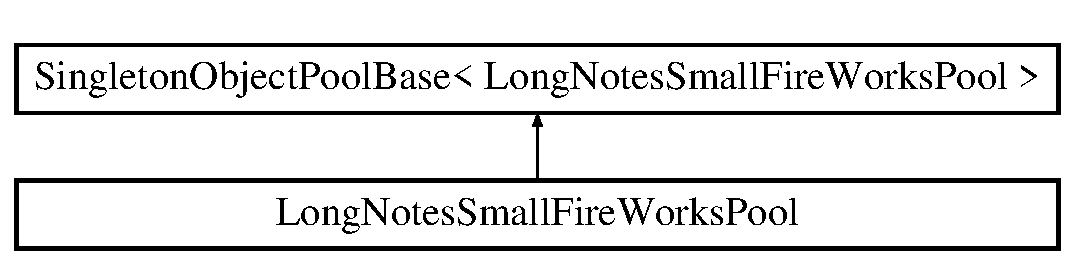
\includegraphics[height=2.000000cm]{class_long_notes_small_fire_works_pool}
\end{center}
\end{figure}
\subsection*{Public Member Functions}
\begin{DoxyCompactItemize}
\item 
void {\bfseries Run} (Vector3 pos)\hypertarget{class_long_notes_small_fire_works_pool_a228be95120dd4ff58bcb0635d6af6651}{}\label{class_long_notes_small_fire_works_pool_a228be95120dd4ff58bcb0635d6af6651}

\end{DoxyCompactItemize}
\subsection*{Additional Inherited Members}


The documentation for this class was generated from the following file\+:\begin{DoxyCompactItemize}
\item 
Scripts/\+Object\+Pool/Long\+Notes\+Small\+Fire\+Works\+Pool.\+cs\end{DoxyCompactItemize}

\hypertarget{class_notes_base}{}\section{Notes\+Base Class Reference}
\label{class_notes_base}\index{Notes\+Base@{Notes\+Base}}


ノーツの基底クラス ///  


Inheritance diagram for Notes\+Base\+:\begin{figure}[H]
\begin{center}
\leavevmode
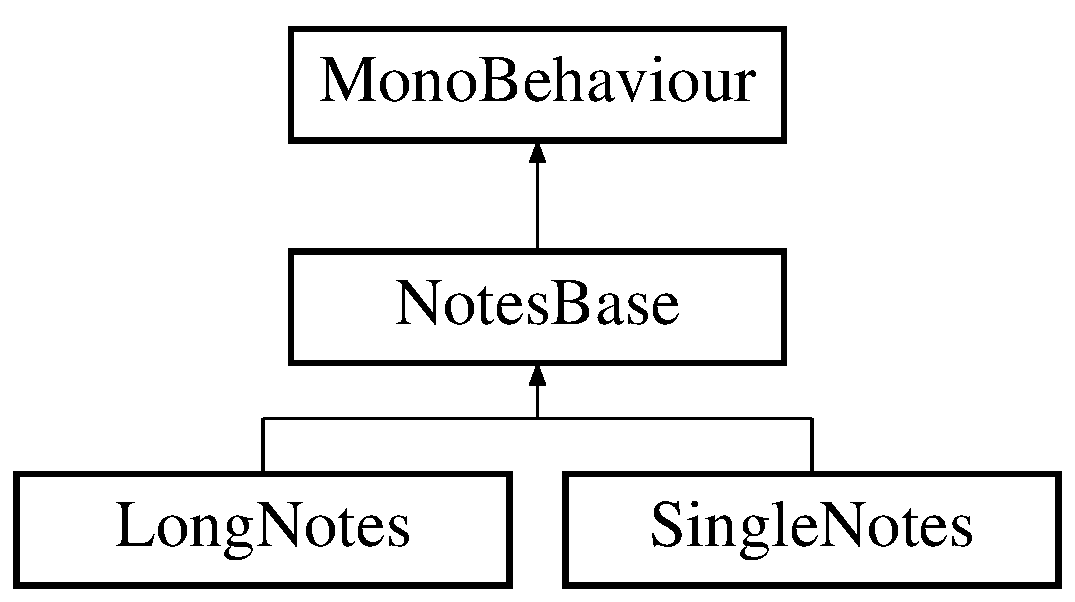
\includegraphics[height=3.000000cm]{class_notes_base}
\end{center}
\end{figure}
\subsection*{Public Member Functions}
\begin{DoxyCompactItemize}
\item 
virtual void {\bfseries Init} (int lane\+No, float down, float up)\hypertarget{class_notes_base_a6060370c8dd6b076c6e735860b069b04}{}\label{class_notes_base_a6060370c8dd6b076c6e735860b069b04}

\item 
virtual void {\bfseries Move} ()\hypertarget{class_notes_base_ab9da30b4b9fddaf96084500d05f78d49}{}\label{class_notes_base_ab9da30b4b9fddaf96084500d05f78d49}

\item 
virtual void {\bfseries Miss} ()\hypertarget{class_notes_base_ab85838d156338efb707228bc318b88a2}{}\label{class_notes_base_ab85838d156338efb707228bc318b88a2}

\item 
virtual void {\bfseries Rec\+Init} (int lane\+No, float down, float up)\hypertarget{class_notes_base_a9875c7d08de04977aebc3431c7356fd4}{}\label{class_notes_base_a9875c7d08de04977aebc3431c7356fd4}

\end{DoxyCompactItemize}
\subsection*{Protected Attributes}
\begin{DoxyCompactItemize}
\item 
const int {\bfseries M\+U\+S\+I\+C\+\_\+\+C\+H\+A\+N\+N\+EL} = 0\hypertarget{class_notes_base_aa1710763eb690be2e6405ef4161526b8}{}\label{class_notes_base_aa1710763eb690be2e6405ef4161526b8}

\item 
const int {\bfseries S\+E\+\_\+\+C\+H\+A\+N\+N\+EL} = 1\hypertarget{class_notes_base_a359a03a7730e3a37db86086a0d1f7a6d}{}\label{class_notes_base_a359a03a7730e3a37db86086a0d1f7a6d}

\end{DoxyCompactItemize}
\subsection*{Properties}
\begin{DoxyCompactItemize}
\item 
virtual float {\bfseries Down\+Time}\hspace{0.3cm}{\ttfamily  \mbox{[}get, set\mbox{]}}\hypertarget{class_notes_base_ac6ddbe1bd315a27b931e43931a4b775f}{}\label{class_notes_base_ac6ddbe1bd315a27b931e43931a4b775f}

\item 
virtual float {\bfseries Up\+Time}\hspace{0.3cm}{\ttfamily  \mbox{[}get, set\mbox{]}}\hypertarget{class_notes_base_ad9f83b6974007661236f97879e9dbe2d}{}\label{class_notes_base_ad9f83b6974007661236f97879e9dbe2d}

\item 
virtual int {\bfseries Lane\+No}\hspace{0.3cm}{\ttfamily  \mbox{[}get, set\mbox{]}}\hypertarget{class_notes_base_a534e0bad053455b72e66c3790d962967}{}\label{class_notes_base_a534e0bad053455b72e66c3790d962967}

\item 
virtual bool {\bfseries is\+Reset}\hspace{0.3cm}{\ttfamily  \mbox{[}get, set\mbox{]}}\hypertarget{class_notes_base_a34bcb4f83f517f356b3dd98e561d192e}{}\label{class_notes_base_a34bcb4f83f517f356b3dd98e561d192e}

\item 
virtual bool {\bfseries is\+Miss}\hspace{0.3cm}{\ttfamily  \mbox{[}get, set\mbox{]}}\hypertarget{class_notes_base_aed65e64d481dc8caf7b8d21c342e9639}{}\label{class_notes_base_aed65e64d481dc8caf7b8d21c342e9639}

\end{DoxyCompactItemize}


\subsection{Detailed Description}
ノーツの基底クラス /// 



The documentation for this class was generated from the following file\+:\begin{DoxyCompactItemize}
\item 
Scripts/\+Notes/Notes\+Base.\+cs\end{DoxyCompactItemize}

\hypertarget{class_notes_manager}{}\section{Notes\+Manager Class Reference}
\label{class_notes_manager}\index{Notes\+Manager@{Notes\+Manager}}


ノーツ管理  


Inheritance diagram for Notes\+Manager\+:\begin{figure}[H]
\begin{center}
\leavevmode
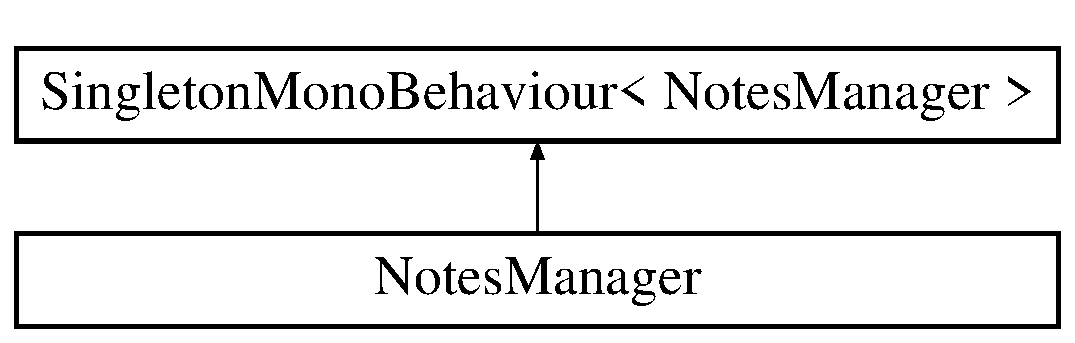
\includegraphics[height=2.000000cm]{class_notes_manager}
\end{center}
\end{figure}
\subsection*{Public Member Functions}
\begin{DoxyCompactItemize}
\item 
void {\bfseries Init} ()\hypertarget{class_notes_manager_a5c7e5c0033598dd87f078fb24397a0bc}{}\label{class_notes_manager_a5c7e5c0033598dd87f078fb24397a0bc}

\item 
void \hyperlink{class_notes_manager_a6f4913237b8e3a4e68f5172f71e51590}{update} ()
\begin{DoxyCompactList}\small\item\em 更新 \end{DoxyCompactList}\item 
void \hyperlink{class_notes_manager_afeb4ec920546b7cc061c50bf2c378f05}{Set\+Notes\+Num} (int num)
\begin{DoxyCompactList}\small\item\em ノーツ総数をセット \end{DoxyCompactList}\item 
void \hyperlink{class_notes_manager_a7be6fd1ad14c143595d4d566cba15442}{Set\+Judge\+Num} (int num)
\begin{DoxyCompactList}\small\item\em 判定するノーツ数をセット ノーツ総数では長押しノーツは1個の扱いだが、 長押しノーツはヘッドとテイルの2個の判定のため判定数は別となる \end{DoxyCompactList}\item 
void \hyperlink{class_notes_manager_a5f5c4538a0d5e8e7cbd9951dddb718d5}{Set\+Notes\+Speed} (float speed)
\begin{DoxyCompactList}\small\item\em ノーツの速度 \end{DoxyCompactList}\item 
void \hyperlink{class_notes_manager_a525cac5533517b75264f0b01b86373d1}{Set\+Active\+Time} (float activate\+Time)
\begin{DoxyCompactList}\small\item\em ノーツのアクティブ時間 \end{DoxyCompactList}\item 
void {\bfseries Set\+Elapsed\+Time} (float time)\hypertarget{class_notes_manager_af3b3d718a9bb6dea98b77836bce7ae99}{}\label{class_notes_manager_af3b3d718a9bb6dea98b77836bce7ae99}

\item 
void \hyperlink{class_notes_manager_a4a2a80e4a52c701ec09c6911cb5e0d2c}{Add\+Notes\+Data} (int id, int point, float down, float up)
\begin{DoxyCompactList}\small\item\em ノーツを構成する追加 \end{DoxyCompactList}\item 
\hyperlink{class_notes_base}{Notes\+Base}\mbox{[}$\,$\mbox{]} \hyperlink{class_notes_manager_ad0f90502e260178cf41ba3ec92cc3fcb}{Get\+Lane\+Area\+Notes} (int lane\+No)
\begin{DoxyCompactList}\small\item\em レーン内のノーツを返す \end{DoxyCompactList}\item 
void \hyperlink{class_notes_manager_a002c55a58d51fb7913a318005fd68edc}{Add\+Perfect\+Score} ()
\begin{DoxyCompactList}\small\item\em 良判定時の加算スコア \end{DoxyCompactList}\item 
void \hyperlink{class_notes_manager_ac6935fc8ab7e7b078f89777355d110ab}{Add\+Great\+Score} ()
\begin{DoxyCompactList}\small\item\em 可判定時の加算スコア \end{DoxyCompactList}\item 
void \hyperlink{class_notes_manager_adcdb5132e598c4d160197c6bfd2ca644}{Add\+Bad\+Score} ()
\begin{DoxyCompactList}\small\item\em 不可判定時の加算スコア \end{DoxyCompactList}\end{DoxyCompactItemize}
\subsection*{Public Attributes}
\begin{DoxyCompactItemize}
\item 
float {\bfseries perfect\+Time} = 0.\+1f\hypertarget{class_notes_manager_af2d67fbf2a1f1aeeb1f77bcdb990bfe4}{}\label{class_notes_manager_af2d67fbf2a1f1aeeb1f77bcdb990bfe4}

\item 
float {\bfseries great\+Time} = 0.\+4f\hypertarget{class_notes_manager_a9fc673597e58d17984e3614ca826fb2b}{}\label{class_notes_manager_a9fc673597e58d17984e3614ca826fb2b}

\item 
float {\bfseries bad\+Time} = 0.\+7f\hypertarget{class_notes_manager_a2873161ada543ab35986a562fca4676f}{}\label{class_notes_manager_a2873161ada543ab35986a562fca4676f}

\end{DoxyCompactItemize}
\subsection*{Properties}
\begin{DoxyCompactItemize}
\item 
float {\bfseries elapsed\+Time}\hspace{0.3cm}{\ttfamily  \mbox{[}get\mbox{]}}\hypertarget{class_notes_manager_a3f0739630828dd12544e9ccd8951c9f6}{}\label{class_notes_manager_a3f0739630828dd12544e9ccd8951c9f6}

\item 
float {\bfseries Reset\+Height}\hspace{0.3cm}{\ttfamily  \mbox{[}get\mbox{]}}\hypertarget{class_notes_manager_aa471b2d457b6f828c82e137f1254caed}{}\label{class_notes_manager_aa471b2d457b6f828c82e137f1254caed}

\item 
float {\bfseries Judge\+Height}\hspace{0.3cm}{\ttfamily  \mbox{[}get\mbox{]}}\hypertarget{class_notes_manager_a6d79946cb97aaf9ec36409655ae13c31}{}\label{class_notes_manager_a6d79946cb97aaf9ec36409655ae13c31}

\item 
float {\bfseries Active\+Time}\hspace{0.3cm}{\ttfamily  \mbox{[}get\mbox{]}}\hypertarget{class_notes_manager_a039913c3746ed4e4cc1712f8a0e09d78}{}\label{class_notes_manager_a039913c3746ed4e4cc1712f8a0e09d78}

\item 
float {\bfseries Speed}\hspace{0.3cm}{\ttfamily  \mbox{[}get\mbox{]}}\hypertarget{class_notes_manager_aa758a63cea01c1160bc179e6b83829c5}{}\label{class_notes_manager_aa758a63cea01c1160bc179e6b83829c5}

\item 
int {\bfseries Notes\+Num}\hspace{0.3cm}{\ttfamily  \mbox{[}get\mbox{]}}\hypertarget{class_notes_manager_aa9d24659a5c5da17b6c0b812fbef0172}{}\label{class_notes_manager_aa9d24659a5c5da17b6c0b812fbef0172}

\item 
int {\bfseries Judge\+Num}\hspace{0.3cm}{\ttfamily  \mbox{[}get\mbox{]}}\hypertarget{class_notes_manager_a10f608cca7565faaa5c445260ccc8db6}{}\label{class_notes_manager_a10f608cca7565faaa5c445260ccc8db6}

\item 
int {\bfseries Success\+Num}\hspace{0.3cm}{\ttfamily  \mbox{[}get, set\mbox{]}}\hypertarget{class_notes_manager_a7ee9c51ee631ee8b2d0acbb94d02e62f}{}\label{class_notes_manager_a7ee9c51ee631ee8b2d0acbb94d02e62f}

\item 
int {\bfseries Now\+Combo}\hspace{0.3cm}{\ttfamily  \mbox{[}get, set\mbox{]}}\hypertarget{class_notes_manager_a7cc3afde1accacb888e538cccdf779e7}{}\label{class_notes_manager_a7cc3afde1accacb888e538cccdf779e7}

\item 
int {\bfseries Max\+Combo}\hspace{0.3cm}{\ttfamily  \mbox{[}get, set\mbox{]}}\hypertarget{class_notes_manager_a03877900f087cdab1b06a79ea784f470}{}\label{class_notes_manager_a03877900f087cdab1b06a79ea784f470}

\item 
int {\bfseries Perfect\+Count}\hspace{0.3cm}{\ttfamily  \mbox{[}get, set\mbox{]}}\hypertarget{class_notes_manager_ab767fa94b954df96b2f7ffa443a3c4b5}{}\label{class_notes_manager_ab767fa94b954df96b2f7ffa443a3c4b5}

\item 
int {\bfseries Great\+Count}\hspace{0.3cm}{\ttfamily  \mbox{[}get, set\mbox{]}}\hypertarget{class_notes_manager_a80c613c1930742c45a71ebff81d4faf8}{}\label{class_notes_manager_a80c613c1930742c45a71ebff81d4faf8}

\item 
int {\bfseries Bad\+Count}\hspace{0.3cm}{\ttfamily  \mbox{[}get, set\mbox{]}}\hypertarget{class_notes_manager_aa89e9356b38044f776adfa30f3e7ee42}{}\label{class_notes_manager_aa89e9356b38044f776adfa30f3e7ee42}

\item 
int {\bfseries Score}\hspace{0.3cm}{\ttfamily  \mbox{[}get\mbox{]}}\hypertarget{class_notes_manager_a72d130f7996ccc91f828b4af01fef1f3}{}\label{class_notes_manager_a72d130f7996ccc91f828b4af01fef1f3}

\end{DoxyCompactItemize}


\subsection{Detailed Description}
ノーツ管理 



\subsection{Member Function Documentation}
\index{Notes\+Manager@{Notes\+Manager}!Add\+Bad\+Score@{Add\+Bad\+Score}}
\index{Add\+Bad\+Score@{Add\+Bad\+Score}!Notes\+Manager@{Notes\+Manager}}
\subsubsection[{\texorpdfstring{Add\+Bad\+Score()}{AddBadScore()}}]{\setlength{\rightskip}{0pt plus 5cm}void Notes\+Manager.\+Add\+Bad\+Score (
\begin{DoxyParamCaption}
{}
\end{DoxyParamCaption}
)\hspace{0.3cm}{\ttfamily [inline]}}\hypertarget{class_notes_manager_adcdb5132e598c4d160197c6bfd2ca644}{}\label{class_notes_manager_adcdb5132e598c4d160197c6bfd2ca644}


不可判定時の加算スコア 

\index{Notes\+Manager@{Notes\+Manager}!Add\+Great\+Score@{Add\+Great\+Score}}
\index{Add\+Great\+Score@{Add\+Great\+Score}!Notes\+Manager@{Notes\+Manager}}
\subsubsection[{\texorpdfstring{Add\+Great\+Score()}{AddGreatScore()}}]{\setlength{\rightskip}{0pt plus 5cm}void Notes\+Manager.\+Add\+Great\+Score (
\begin{DoxyParamCaption}
{}
\end{DoxyParamCaption}
)\hspace{0.3cm}{\ttfamily [inline]}}\hypertarget{class_notes_manager_ac6935fc8ab7e7b078f89777355d110ab}{}\label{class_notes_manager_ac6935fc8ab7e7b078f89777355d110ab}


可判定時の加算スコア 

\index{Notes\+Manager@{Notes\+Manager}!Add\+Notes\+Data@{Add\+Notes\+Data}}
\index{Add\+Notes\+Data@{Add\+Notes\+Data}!Notes\+Manager@{Notes\+Manager}}
\subsubsection[{\texorpdfstring{Add\+Notes\+Data(int id, int point, float down, float up)}{AddNotesData(int id, int point, float down, float up)}}]{\setlength{\rightskip}{0pt plus 5cm}void Notes\+Manager.\+Add\+Notes\+Data (
\begin{DoxyParamCaption}
\item[{int}]{id, }
\item[{int}]{point, }
\item[{float}]{down, }
\item[{float}]{up}
\end{DoxyParamCaption}
)\hspace{0.3cm}{\ttfamily [inline]}}\hypertarget{class_notes_manager_a4a2a80e4a52c701ec09c6911cb5e0d2c}{}\label{class_notes_manager_a4a2a80e4a52c701ec09c6911cb5e0d2c}


ノーツを構成する追加 


\begin{DoxyParams}{Parameters}
{\em id} & \\
\hline
{\em point} & \\
\hline
{\em down} & \\
\hline
{\em up} & \\
\hline
\end{DoxyParams}
\index{Notes\+Manager@{Notes\+Manager}!Add\+Perfect\+Score@{Add\+Perfect\+Score}}
\index{Add\+Perfect\+Score@{Add\+Perfect\+Score}!Notes\+Manager@{Notes\+Manager}}
\subsubsection[{\texorpdfstring{Add\+Perfect\+Score()}{AddPerfectScore()}}]{\setlength{\rightskip}{0pt plus 5cm}void Notes\+Manager.\+Add\+Perfect\+Score (
\begin{DoxyParamCaption}
{}
\end{DoxyParamCaption}
)\hspace{0.3cm}{\ttfamily [inline]}}\hypertarget{class_notes_manager_a002c55a58d51fb7913a318005fd68edc}{}\label{class_notes_manager_a002c55a58d51fb7913a318005fd68edc}


良判定時の加算スコア 

\index{Notes\+Manager@{Notes\+Manager}!Get\+Lane\+Area\+Notes@{Get\+Lane\+Area\+Notes}}
\index{Get\+Lane\+Area\+Notes@{Get\+Lane\+Area\+Notes}!Notes\+Manager@{Notes\+Manager}}
\subsubsection[{\texorpdfstring{Get\+Lane\+Area\+Notes(int lane\+No)}{GetLaneAreaNotes(int laneNo)}}]{\setlength{\rightskip}{0pt plus 5cm}{\bf Notes\+Base} \mbox{[}$\,$\mbox{]} Notes\+Manager.\+Get\+Lane\+Area\+Notes (
\begin{DoxyParamCaption}
\item[{int}]{lane\+No}
\end{DoxyParamCaption}
)\hspace{0.3cm}{\ttfamily [inline]}}\hypertarget{class_notes_manager_ad0f90502e260178cf41ba3ec92cc3fcb}{}\label{class_notes_manager_ad0f90502e260178cf41ba3ec92cc3fcb}


レーン内のノーツを返す 


\begin{DoxyParams}{Parameters}
{\em lane\+No} & \\
\hline
\end{DoxyParams}
\begin{DoxyReturn}{Returns}

\end{DoxyReturn}
\index{Notes\+Manager@{Notes\+Manager}!Set\+Active\+Time@{Set\+Active\+Time}}
\index{Set\+Active\+Time@{Set\+Active\+Time}!Notes\+Manager@{Notes\+Manager}}
\subsubsection[{\texorpdfstring{Set\+Active\+Time(float activate\+Time)}{SetActiveTime(float activateTime)}}]{\setlength{\rightskip}{0pt plus 5cm}void Notes\+Manager.\+Set\+Active\+Time (
\begin{DoxyParamCaption}
\item[{float}]{activate\+Time}
\end{DoxyParamCaption}
)\hspace{0.3cm}{\ttfamily [inline]}}\hypertarget{class_notes_manager_a525cac5533517b75264f0b01b86373d1}{}\label{class_notes_manager_a525cac5533517b75264f0b01b86373d1}


ノーツのアクティブ時間 


\begin{DoxyParams}{Parameters}
{\em activate\+Time} & \\
\hline
\end{DoxyParams}
\index{Notes\+Manager@{Notes\+Manager}!Set\+Judge\+Num@{Set\+Judge\+Num}}
\index{Set\+Judge\+Num@{Set\+Judge\+Num}!Notes\+Manager@{Notes\+Manager}}
\subsubsection[{\texorpdfstring{Set\+Judge\+Num(int num)}{SetJudgeNum(int num)}}]{\setlength{\rightskip}{0pt plus 5cm}void Notes\+Manager.\+Set\+Judge\+Num (
\begin{DoxyParamCaption}
\item[{int}]{num}
\end{DoxyParamCaption}
)\hspace{0.3cm}{\ttfamily [inline]}}\hypertarget{class_notes_manager_a7be6fd1ad14c143595d4d566cba15442}{}\label{class_notes_manager_a7be6fd1ad14c143595d4d566cba15442}


判定するノーツ数をセット ノーツ総数では長押しノーツは1個の扱いだが、 長押しノーツはヘッドとテイルの2個の判定のため判定数は別となる 


\begin{DoxyParams}{Parameters}
{\em num} & \\
\hline
\end{DoxyParams}
\index{Notes\+Manager@{Notes\+Manager}!Set\+Notes\+Num@{Set\+Notes\+Num}}
\index{Set\+Notes\+Num@{Set\+Notes\+Num}!Notes\+Manager@{Notes\+Manager}}
\subsubsection[{\texorpdfstring{Set\+Notes\+Num(int num)}{SetNotesNum(int num)}}]{\setlength{\rightskip}{0pt plus 5cm}void Notes\+Manager.\+Set\+Notes\+Num (
\begin{DoxyParamCaption}
\item[{int}]{num}
\end{DoxyParamCaption}
)\hspace{0.3cm}{\ttfamily [inline]}}\hypertarget{class_notes_manager_afeb4ec920546b7cc061c50bf2c378f05}{}\label{class_notes_manager_afeb4ec920546b7cc061c50bf2c378f05}


ノーツ総数をセット 


\begin{DoxyParams}{Parameters}
{\em num} & \\
\hline
\end{DoxyParams}
\index{Notes\+Manager@{Notes\+Manager}!Set\+Notes\+Speed@{Set\+Notes\+Speed}}
\index{Set\+Notes\+Speed@{Set\+Notes\+Speed}!Notes\+Manager@{Notes\+Manager}}
\subsubsection[{\texorpdfstring{Set\+Notes\+Speed(float speed)}{SetNotesSpeed(float speed)}}]{\setlength{\rightskip}{0pt plus 5cm}void Notes\+Manager.\+Set\+Notes\+Speed (
\begin{DoxyParamCaption}
\item[{float}]{speed}
\end{DoxyParamCaption}
)\hspace{0.3cm}{\ttfamily [inline]}}\hypertarget{class_notes_manager_a5f5c4538a0d5e8e7cbd9951dddb718d5}{}\label{class_notes_manager_a5f5c4538a0d5e8e7cbd9951dddb718d5}


ノーツの速度 


\begin{DoxyParams}{Parameters}
{\em speed} & \\
\hline
\end{DoxyParams}
\index{Notes\+Manager@{Notes\+Manager}!update@{update}}
\index{update@{update}!Notes\+Manager@{Notes\+Manager}}
\subsubsection[{\texorpdfstring{update()}{update()}}]{\setlength{\rightskip}{0pt plus 5cm}void Notes\+Manager.\+update (
\begin{DoxyParamCaption}
{}
\end{DoxyParamCaption}
)\hspace{0.3cm}{\ttfamily [inline]}}\hypertarget{class_notes_manager_a6f4913237b8e3a4e68f5172f71e51590}{}\label{class_notes_manager_a6f4913237b8e3a4e68f5172f71e51590}


更新 



The documentation for this class was generated from the following file\+:\begin{DoxyCompactItemize}
\item 
Scripts/\+Notes/Notes\+Manager.\+cs\end{DoxyCompactItemize}

\hypertarget{class_pause_control}{}\section{Pause\+Control Class Reference}
\label{class_pause_control}\index{Pause\+Control@{Pause\+Control}}


ポーズのコントロール  


Inheritance diagram for Pause\+Control\+:\begin{figure}[H]
\begin{center}
\leavevmode
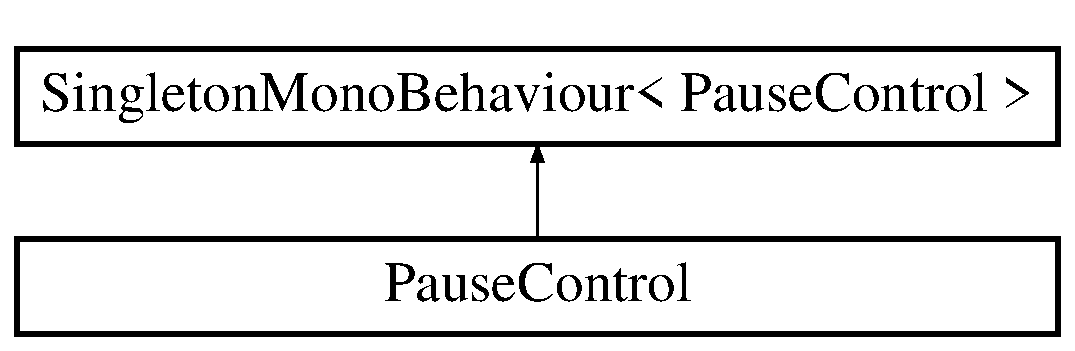
\includegraphics[height=2.000000cm]{class_pause_control}
\end{center}
\end{figure}
\subsection*{Public Member Functions}
\begin{DoxyCompactItemize}
\item 
void {\bfseries Init} ()\hypertarget{class_pause_control_ab740dcc52a22cafa069e741a53b35b05}{}\label{class_pause_control_ab740dcc52a22cafa069e741a53b35b05}

\item 
void {\bfseries update} ()\hypertarget{class_pause_control_aee921761115f4a7a358989f4353de382}{}\label{class_pause_control_aee921761115f4a7a358989f4353de382}

\item 
void \hyperlink{class_pause_control_ae6ddd7c5a8341174cff9750d195edcf1}{On\+Touch\+Pause} ()
\begin{DoxyCompactList}\small\item\em ポーズにタッチ \end{DoxyCompactList}\item 
void \hyperlink{class_pause_control_a755b026ed1df770b94f3f04c74c1956b}{Open} ()
\begin{DoxyCompactList}\small\item\em ポーズを開く処理 \end{DoxyCompactList}\item 
void \hyperlink{class_pause_control_ab4a86be3d5d84c0b042f608a493dbe50}{Close} ()
\begin{DoxyCompactList}\small\item\em ポーズを閉じる処理 \end{DoxyCompactList}\item 
void \hyperlink{class_pause_control_a97be9c0cd95af026fa75760e96f824cc}{Return\+Title} ()
\begin{DoxyCompactList}\small\item\em タイトルに戻る処理 \end{DoxyCompactList}\item 
void \hyperlink{class_pause_control_aeedeaa20e5b1508183439c4172cbbec0}{Return\+Music\+Select} ()
\begin{DoxyCompactList}\small\item\em セレクトに戻る処理 \end{DoxyCompactList}\end{DoxyCompactItemize}
\subsection*{Additional Inherited Members}


\subsection{Detailed Description}
ポーズのコントロール 



\subsection{Member Function Documentation}
\index{Pause\+Control@{Pause\+Control}!Close@{Close}}
\index{Close@{Close}!Pause\+Control@{Pause\+Control}}
\subsubsection[{\texorpdfstring{Close()}{Close()}}]{\setlength{\rightskip}{0pt plus 5cm}void Pause\+Control.\+Close (
\begin{DoxyParamCaption}
{}
\end{DoxyParamCaption}
)\hspace{0.3cm}{\ttfamily [inline]}}\hypertarget{class_pause_control_ab4a86be3d5d84c0b042f608a493dbe50}{}\label{class_pause_control_ab4a86be3d5d84c0b042f608a493dbe50}


ポーズを閉じる処理 

\index{Pause\+Control@{Pause\+Control}!On\+Touch\+Pause@{On\+Touch\+Pause}}
\index{On\+Touch\+Pause@{On\+Touch\+Pause}!Pause\+Control@{Pause\+Control}}
\subsubsection[{\texorpdfstring{On\+Touch\+Pause()}{OnTouchPause()}}]{\setlength{\rightskip}{0pt plus 5cm}void Pause\+Control.\+On\+Touch\+Pause (
\begin{DoxyParamCaption}
{}
\end{DoxyParamCaption}
)\hspace{0.3cm}{\ttfamily [inline]}}\hypertarget{class_pause_control_ae6ddd7c5a8341174cff9750d195edcf1}{}\label{class_pause_control_ae6ddd7c5a8341174cff9750d195edcf1}


ポーズにタッチ 

\index{Pause\+Control@{Pause\+Control}!Open@{Open}}
\index{Open@{Open}!Pause\+Control@{Pause\+Control}}
\subsubsection[{\texorpdfstring{Open()}{Open()}}]{\setlength{\rightskip}{0pt plus 5cm}void Pause\+Control.\+Open (
\begin{DoxyParamCaption}
{}
\end{DoxyParamCaption}
)\hspace{0.3cm}{\ttfamily [inline]}}\hypertarget{class_pause_control_a755b026ed1df770b94f3f04c74c1956b}{}\label{class_pause_control_a755b026ed1df770b94f3f04c74c1956b}


ポーズを開く処理 

\index{Pause\+Control@{Pause\+Control}!Return\+Music\+Select@{Return\+Music\+Select}}
\index{Return\+Music\+Select@{Return\+Music\+Select}!Pause\+Control@{Pause\+Control}}
\subsubsection[{\texorpdfstring{Return\+Music\+Select()}{ReturnMusicSelect()}}]{\setlength{\rightskip}{0pt plus 5cm}void Pause\+Control.\+Return\+Music\+Select (
\begin{DoxyParamCaption}
{}
\end{DoxyParamCaption}
)\hspace{0.3cm}{\ttfamily [inline]}}\hypertarget{class_pause_control_aeedeaa20e5b1508183439c4172cbbec0}{}\label{class_pause_control_aeedeaa20e5b1508183439c4172cbbec0}


セレクトに戻る処理 

\index{Pause\+Control@{Pause\+Control}!Return\+Title@{Return\+Title}}
\index{Return\+Title@{Return\+Title}!Pause\+Control@{Pause\+Control}}
\subsubsection[{\texorpdfstring{Return\+Title()}{ReturnTitle()}}]{\setlength{\rightskip}{0pt plus 5cm}void Pause\+Control.\+Return\+Title (
\begin{DoxyParamCaption}
{}
\end{DoxyParamCaption}
)\hspace{0.3cm}{\ttfamily [inline]}}\hypertarget{class_pause_control_a97be9c0cd95af026fa75760e96f824cc}{}\label{class_pause_control_a97be9c0cd95af026fa75760e96f824cc}


タイトルに戻る処理 



The documentation for this class was generated from the following file\+:\begin{DoxyCompactItemize}
\item 
Scripts/\+Pause/Pause\+Control.\+cs\end{DoxyCompactItemize}

\hypertarget{class_play_data}{}\section{Play\+Data Class Reference}
\label{class_play_data}\index{Play\+Data@{Play\+Data}}


楽曲プレイするにあたって保存しておかないといけないデータ群  


Inheritance diagram for Play\+Data\+:\begin{figure}[H]
\begin{center}
\leavevmode
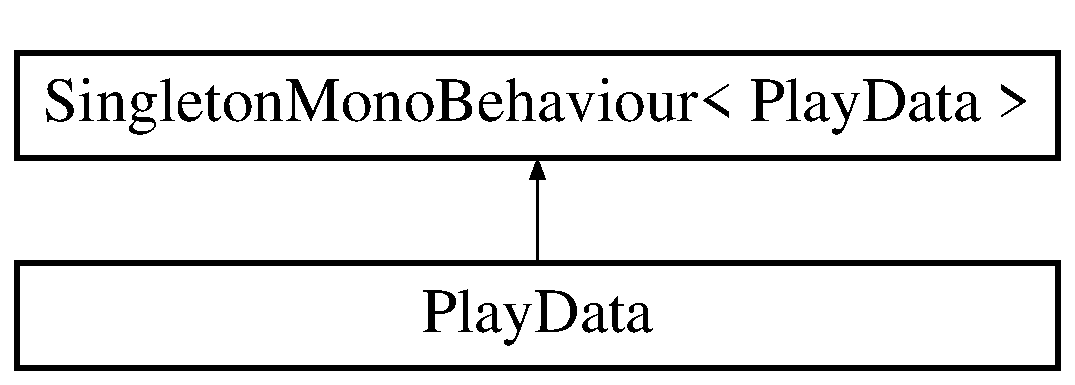
\includegraphics[height=2.000000cm]{class_play_data}
\end{center}
\end{figure}
\subsection*{Public Types}
\begin{DoxyCompactItemize}
\item 
enum {\bfseries Level} \{ {\bfseries Easy}, 
{\bfseries Normal}, 
{\bfseries Hard}
 \}\hypertarget{class_play_data_a3561a38cd6b282fd2f39b0e0c458c032}{}\label{class_play_data_a3561a38cd6b282fd2f39b0e0c458c032}

\item 
enum {\bfseries Speed} \{ \\*
{\bfseries O\+NE} = 1, 
{\bfseries T\+WO}, 
{\bfseries T\+H\+R\+EE}, 
{\bfseries F\+O\+UR}, 
\\*
{\bfseries F\+I\+VE}, 
{\bfseries S\+IX}, 
{\bfseries S\+E\+V\+EN}, 
{\bfseries E\+I\+G\+HT}, 
\\*
{\bfseries N\+I\+NE}, 
{\bfseries T\+EN}
 \}\hypertarget{class_play_data_a5273921272a1cf4ea28646ea538b48f4}{}\label{class_play_data_a5273921272a1cf4ea28646ea538b48f4}

\item 
enum {\bfseries Volume} \{ \\*
{\bfseries Z\+E\+RO}, 
{\bfseries O\+NE}, 
{\bfseries T\+WO}, 
{\bfseries T\+H\+R\+EE}, 
\\*
{\bfseries F\+O\+UR}, 
{\bfseries F\+I\+VE}, 
{\bfseries S\+IX}, 
{\bfseries S\+E\+V\+EN}, 
\\*
{\bfseries E\+I\+G\+HT}, 
{\bfseries N\+I\+NE}, 
{\bfseries T\+EN}
 \}\hypertarget{class_play_data_a879920467d76bd3a858c9c2025e98659}{}\label{class_play_data_a879920467d76bd3a858c9c2025e98659}

\end{DoxyCompactItemize}
\subsection*{Public Member Functions}
\begin{DoxyCompactItemize}
\item 
void \hyperlink{class_play_data_a67575e29933665c60e5f60135875bb69}{Set\+Level} (Level level)
\begin{DoxyCompactList}\small\item\em 難易度の設定 \end{DoxyCompactList}\item 
void \hyperlink{class_play_data_a3840f7faaa54b86ff3ec207ef85b7033}{Reset\+Data} ()
\begin{DoxyCompactList}\small\item\em データのリセット \end{DoxyCompactList}\item 
void \hyperlink{class_play_data_af935b9627b1aed55166d3b67433d1c04}{Add\+Speed} ()
\begin{DoxyCompactList}\small\item\em 速度上昇 \end{DoxyCompactList}\item 
void \hyperlink{class_play_data_a3daf8700808d898b695b4394d5086113}{Add\+S\+E\+Volume} ()
\begin{DoxyCompactList}\small\item\em S\+Eの音量の上昇 \end{DoxyCompactList}\item 
void \hyperlink{class_play_data_a22fd27b0cd3c566ceb2383db1ff01583}{Add\+B\+G\+M\+Volume} ()
\begin{DoxyCompactList}\small\item\em B\+G\+Mの音量の上昇 \end{DoxyCompactList}\item 
void \hyperlink{class_play_data_a3aaf96876ca0992bc7170d81725de4dc}{Less\+Speed} ()
\begin{DoxyCompactList}\small\item\em 速度減少 \end{DoxyCompactList}\item 
void \hyperlink{class_play_data_afa4ccf849600e4cd54da901338f537af}{Less\+S\+E\+Volume} ()
\begin{DoxyCompactList}\small\item\em S\+Eの音量の減少 \end{DoxyCompactList}\item 
void \hyperlink{class_play_data_a74919d0b214b27b6f99f6f12ae45e288}{Less\+B\+G\+M\+Volume} ()
\begin{DoxyCompactList}\small\item\em B\+G\+Mの音量の減少 \end{DoxyCompactList}\item 
void \hyperlink{class_play_data_af321c45a332a001cf564dc34fbf6d200}{Set\+Play\+Data} ()
\begin{DoxyCompactList}\small\item\em プレイデータ(ノーツスピード、プール数、プールタイム)のセット \end{DoxyCompactList}\item 
I\+Enumerator \hyperlink{class_play_data_a7af0781e257708ef6ee6a02eb56984c4}{Load\+System\+Data} ()
\begin{DoxyCompactList}\small\item\em システムデータの読み込み \end{DoxyCompactList}\item 
void {\bfseries Write\+System\+Data} ()\hypertarget{class_play_data_a86f121114610b5e2fe2b580a737aae69}{}\label{class_play_data_a86f121114610b5e2fe2b580a737aae69}

\item 
void \hyperlink{class_play_data_a6bc6a5c0b10fe2b7089b4ee043f42c89}{Write\+System\+Data} (float se\+Vol, float bgm\+Vol, Speed speed)
\begin{DoxyCompactList}\small\item\em システムデータの書き込み 既にデータがあるはずなのですでにあるものはいったん削除する \end{DoxyCompactList}\end{DoxyCompactItemize}
\subsection*{Public Attributes}
\begin{DoxyCompactItemize}
\item 
const Speed {\bfseries M\+A\+X\+\_\+\+S\+P\+E\+ED} = Speed.\+T\+EN\hypertarget{class_play_data_ad26af255954f87a3e38714c4c52e883b}{}\label{class_play_data_ad26af255954f87a3e38714c4c52e883b}

\item 
const Speed {\bfseries M\+I\+N\+\_\+\+S\+P\+E\+ED} = Speed.\+O\+NE\hypertarget{class_play_data_a59d69a6f1920500d17c31929668d039a}{}\label{class_play_data_a59d69a6f1920500d17c31929668d039a}

\item 
const Volume {\bfseries M\+A\+X\+\_\+\+V\+O\+L\+U\+ME} = Volume.\+T\+EN\hypertarget{class_play_data_ab6ae016cf4a9eb1c28c37405eeb7d2f5}{}\label{class_play_data_ab6ae016cf4a9eb1c28c37405eeb7d2f5}

\item 
const Volume {\bfseries M\+I\+N\+\_\+\+V\+O\+L\+U\+ME} = Volume.\+Z\+E\+RO\hypertarget{class_play_data_a924b81bf46539693eeff9a9776871b09}{}\label{class_play_data_a924b81bf46539693eeff9a9776871b09}

\item 
const string {\bfseries System\+Path} = \char`\"{}system.\+ini\char`\"{}\hypertarget{class_play_data_aec36a92cc8887da39f8152b22419160c}{}\label{class_play_data_aec36a92cc8887da39f8152b22419160c}

\end{DoxyCompactItemize}
\subsection*{Properties}
\begin{DoxyCompactItemize}
\item 
Level {\bfseries level}\hspace{0.3cm}{\ttfamily  \mbox{[}get\mbox{]}}\hypertarget{class_play_data_a87e4d5b2a29d3078721c3b12c9247f20}{}\label{class_play_data_a87e4d5b2a29d3078721c3b12c9247f20}

\item 
Speed {\bfseries speed}\hspace{0.3cm}{\ttfamily  \mbox{[}get\mbox{]}}\hypertarget{class_play_data_acf07fcdd3d91262ed31b68cbf0327899}{}\label{class_play_data_acf07fcdd3d91262ed31b68cbf0327899}

\item 
float {\bfseries notes\+Speed}\hspace{0.3cm}{\ttfamily  \mbox{[}get\mbox{]}}\hypertarget{class_play_data_a20f638eaa95e6f7a41a318bc21e1023c}{}\label{class_play_data_a20f638eaa95e6f7a41a318bc21e1023c}

\item 
Volume {\bfseries S\+E\+Vol}\hspace{0.3cm}{\ttfamily  \mbox{[}get\mbox{]}}\hypertarget{class_play_data_aca9ae040610b815c9047f8d621619cd8}{}\label{class_play_data_aca9ae040610b815c9047f8d621619cd8}

\item 
Volume {\bfseries B\+G\+M\+Vol}\hspace{0.3cm}{\ttfamily  \mbox{[}get\mbox{]}}\hypertarget{class_play_data_a5e369ebd76206ba182b9836d57d60518}{}\label{class_play_data_a5e369ebd76206ba182b9836d57d60518}

\item 
float {\bfseries S\+E\+Vol\+Value}\hspace{0.3cm}{\ttfamily  \mbox{[}get\mbox{]}}\hypertarget{class_play_data_ae2efe6ff299c518d181ce04ce7cd9765}{}\label{class_play_data_ae2efe6ff299c518d181ce04ce7cd9765}

\item 
float {\bfseries B\+G\+M\+Vol\+Value}\hspace{0.3cm}{\ttfamily  \mbox{[}get\mbox{]}}\hypertarget{class_play_data_a5fe9593b45154a8ca1862c7d91f2915a}{}\label{class_play_data_a5fe9593b45154a8ca1862c7d91f2915a}

\item 
float {\bfseries Notes\+Active\+Time}\hspace{0.3cm}{\ttfamily  \mbox{[}get\mbox{]}}\hypertarget{class_play_data_a8665728805d4db8a7726a6c70633a8ef}{}\label{class_play_data_a8665728805d4db8a7726a6c70633a8ef}

\item 
int {\bfseries simple\+Notes\+Pool\+Num}\hspace{0.3cm}{\ttfamily  \mbox{[}get\mbox{]}}\hypertarget{class_play_data_a0c0e8f086a8a02aeaad6c404a239368f}{}\label{class_play_data_a0c0e8f086a8a02aeaad6c404a239368f}

\item 
string {\bfseries file\+Path}\hspace{0.3cm}{\ttfamily  \mbox{[}get\mbox{]}}\hypertarget{class_play_data_ad5bbccf74a246e45fcdc89fac9c093b0}{}\label{class_play_data_ad5bbccf74a246e45fcdc89fac9c093b0}

\end{DoxyCompactItemize}


\subsection{Detailed Description}
楽曲プレイするにあたって保存しておかないといけないデータ群 



\subsection{Member Function Documentation}
\index{Play\+Data@{Play\+Data}!Add\+B\+G\+M\+Volume@{Add\+B\+G\+M\+Volume}}
\index{Add\+B\+G\+M\+Volume@{Add\+B\+G\+M\+Volume}!Play\+Data@{Play\+Data}}
\subsubsection[{\texorpdfstring{Add\+B\+G\+M\+Volume()}{AddBGMVolume()}}]{\setlength{\rightskip}{0pt plus 5cm}void Play\+Data.\+Add\+B\+G\+M\+Volume (
\begin{DoxyParamCaption}
{}
\end{DoxyParamCaption}
)\hspace{0.3cm}{\ttfamily [inline]}}\hypertarget{class_play_data_a22fd27b0cd3c566ceb2383db1ff01583}{}\label{class_play_data_a22fd27b0cd3c566ceb2383db1ff01583}


B\+G\+Mの音量の上昇 

\index{Play\+Data@{Play\+Data}!Add\+S\+E\+Volume@{Add\+S\+E\+Volume}}
\index{Add\+S\+E\+Volume@{Add\+S\+E\+Volume}!Play\+Data@{Play\+Data}}
\subsubsection[{\texorpdfstring{Add\+S\+E\+Volume()}{AddSEVolume()}}]{\setlength{\rightskip}{0pt plus 5cm}void Play\+Data.\+Add\+S\+E\+Volume (
\begin{DoxyParamCaption}
{}
\end{DoxyParamCaption}
)\hspace{0.3cm}{\ttfamily [inline]}}\hypertarget{class_play_data_a3daf8700808d898b695b4394d5086113}{}\label{class_play_data_a3daf8700808d898b695b4394d5086113}


S\+Eの音量の上昇 

\index{Play\+Data@{Play\+Data}!Add\+Speed@{Add\+Speed}}
\index{Add\+Speed@{Add\+Speed}!Play\+Data@{Play\+Data}}
\subsubsection[{\texorpdfstring{Add\+Speed()}{AddSpeed()}}]{\setlength{\rightskip}{0pt plus 5cm}void Play\+Data.\+Add\+Speed (
\begin{DoxyParamCaption}
{}
\end{DoxyParamCaption}
)\hspace{0.3cm}{\ttfamily [inline]}}\hypertarget{class_play_data_af935b9627b1aed55166d3b67433d1c04}{}\label{class_play_data_af935b9627b1aed55166d3b67433d1c04}


速度上昇 

\index{Play\+Data@{Play\+Data}!Less\+B\+G\+M\+Volume@{Less\+B\+G\+M\+Volume}}
\index{Less\+B\+G\+M\+Volume@{Less\+B\+G\+M\+Volume}!Play\+Data@{Play\+Data}}
\subsubsection[{\texorpdfstring{Less\+B\+G\+M\+Volume()}{LessBGMVolume()}}]{\setlength{\rightskip}{0pt plus 5cm}void Play\+Data.\+Less\+B\+G\+M\+Volume (
\begin{DoxyParamCaption}
{}
\end{DoxyParamCaption}
)\hspace{0.3cm}{\ttfamily [inline]}}\hypertarget{class_play_data_a74919d0b214b27b6f99f6f12ae45e288}{}\label{class_play_data_a74919d0b214b27b6f99f6f12ae45e288}


B\+G\+Mの音量の減少 

\index{Play\+Data@{Play\+Data}!Less\+S\+E\+Volume@{Less\+S\+E\+Volume}}
\index{Less\+S\+E\+Volume@{Less\+S\+E\+Volume}!Play\+Data@{Play\+Data}}
\subsubsection[{\texorpdfstring{Less\+S\+E\+Volume()}{LessSEVolume()}}]{\setlength{\rightskip}{0pt plus 5cm}void Play\+Data.\+Less\+S\+E\+Volume (
\begin{DoxyParamCaption}
{}
\end{DoxyParamCaption}
)\hspace{0.3cm}{\ttfamily [inline]}}\hypertarget{class_play_data_afa4ccf849600e4cd54da901338f537af}{}\label{class_play_data_afa4ccf849600e4cd54da901338f537af}


S\+Eの音量の減少 

\index{Play\+Data@{Play\+Data}!Less\+Speed@{Less\+Speed}}
\index{Less\+Speed@{Less\+Speed}!Play\+Data@{Play\+Data}}
\subsubsection[{\texorpdfstring{Less\+Speed()}{LessSpeed()}}]{\setlength{\rightskip}{0pt plus 5cm}void Play\+Data.\+Less\+Speed (
\begin{DoxyParamCaption}
{}
\end{DoxyParamCaption}
)\hspace{0.3cm}{\ttfamily [inline]}}\hypertarget{class_play_data_a3aaf96876ca0992bc7170d81725de4dc}{}\label{class_play_data_a3aaf96876ca0992bc7170d81725de4dc}


速度減少 

\index{Play\+Data@{Play\+Data}!Load\+System\+Data@{Load\+System\+Data}}
\index{Load\+System\+Data@{Load\+System\+Data}!Play\+Data@{Play\+Data}}
\subsubsection[{\texorpdfstring{Load\+System\+Data()}{LoadSystemData()}}]{\setlength{\rightskip}{0pt plus 5cm}I\+Enumerator Play\+Data.\+Load\+System\+Data (
\begin{DoxyParamCaption}
{}
\end{DoxyParamCaption}
)\hspace{0.3cm}{\ttfamily [inline]}}\hypertarget{class_play_data_a7af0781e257708ef6ee6a02eb56984c4}{}\label{class_play_data_a7af0781e257708ef6ee6a02eb56984c4}


システムデータの読み込み 

\begin{DoxyReturn}{Returns}

\end{DoxyReturn}
\index{Play\+Data@{Play\+Data}!Reset\+Data@{Reset\+Data}}
\index{Reset\+Data@{Reset\+Data}!Play\+Data@{Play\+Data}}
\subsubsection[{\texorpdfstring{Reset\+Data()}{ResetData()}}]{\setlength{\rightskip}{0pt plus 5cm}void Play\+Data.\+Reset\+Data (
\begin{DoxyParamCaption}
{}
\end{DoxyParamCaption}
)\hspace{0.3cm}{\ttfamily [inline]}}\hypertarget{class_play_data_a3840f7faaa54b86ff3ec207ef85b7033}{}\label{class_play_data_a3840f7faaa54b86ff3ec207ef85b7033}


データのリセット 

\index{Play\+Data@{Play\+Data}!Set\+Level@{Set\+Level}}
\index{Set\+Level@{Set\+Level}!Play\+Data@{Play\+Data}}
\subsubsection[{\texorpdfstring{Set\+Level(\+Level level)}{SetLevel(Level level)}}]{\setlength{\rightskip}{0pt plus 5cm}void Play\+Data.\+Set\+Level (
\begin{DoxyParamCaption}
\item[{Level}]{level}
\end{DoxyParamCaption}
)\hspace{0.3cm}{\ttfamily [inline]}}\hypertarget{class_play_data_a67575e29933665c60e5f60135875bb69}{}\label{class_play_data_a67575e29933665c60e5f60135875bb69}


難易度の設定 


\begin{DoxyParams}{Parameters}
{\em level} & \\
\hline
\end{DoxyParams}
\index{Play\+Data@{Play\+Data}!Set\+Play\+Data@{Set\+Play\+Data}}
\index{Set\+Play\+Data@{Set\+Play\+Data}!Play\+Data@{Play\+Data}}
\subsubsection[{\texorpdfstring{Set\+Play\+Data()}{SetPlayData()}}]{\setlength{\rightskip}{0pt plus 5cm}void Play\+Data.\+Set\+Play\+Data (
\begin{DoxyParamCaption}
{}
\end{DoxyParamCaption}
)\hspace{0.3cm}{\ttfamily [inline]}}\hypertarget{class_play_data_af321c45a332a001cf564dc34fbf6d200}{}\label{class_play_data_af321c45a332a001cf564dc34fbf6d200}


プレイデータ(ノーツスピード、プール数、プールタイム)のセット 

\index{Play\+Data@{Play\+Data}!Write\+System\+Data@{Write\+System\+Data}}
\index{Write\+System\+Data@{Write\+System\+Data}!Play\+Data@{Play\+Data}}
\subsubsection[{\texorpdfstring{Write\+System\+Data(float se\+Vol, float bgm\+Vol, Speed speed)}{WriteSystemData(float seVol, float bgmVol, Speed speed)}}]{\setlength{\rightskip}{0pt plus 5cm}void Play\+Data.\+Write\+System\+Data (
\begin{DoxyParamCaption}
\item[{float}]{se\+Vol, }
\item[{float}]{bgm\+Vol, }
\item[{Speed}]{speed}
\end{DoxyParamCaption}
)\hspace{0.3cm}{\ttfamily [inline]}}\hypertarget{class_play_data_a6bc6a5c0b10fe2b7089b4ee043f42c89}{}\label{class_play_data_a6bc6a5c0b10fe2b7089b4ee043f42c89}


システムデータの書き込み 既にデータがあるはずなのですでにあるものはいったん削除する 


\begin{DoxyParams}{Parameters}
{\em se\+Vol} & \\
\hline
{\em bgm\+Vol} & \\
\hline
{\em speed} & \\
\hline
\end{DoxyParams}


The documentation for this class was generated from the following file\+:\begin{DoxyCompactItemize}
\item 
Scripts/\+Play\+Data/Play\+Data.\+cs\end{DoxyCompactItemize}

\hypertarget{class_push_sprite_box}{}\section{Push\+Sprite\+Box Class Reference}
\label{class_push_sprite_box}\index{Push\+Sprite\+Box@{Push\+Sprite\+Box}}


四角形の当たり判定を持ったスプライト  


Inheritance diagram for Push\+Sprite\+Box\+:\begin{figure}[H]
\begin{center}
\leavevmode
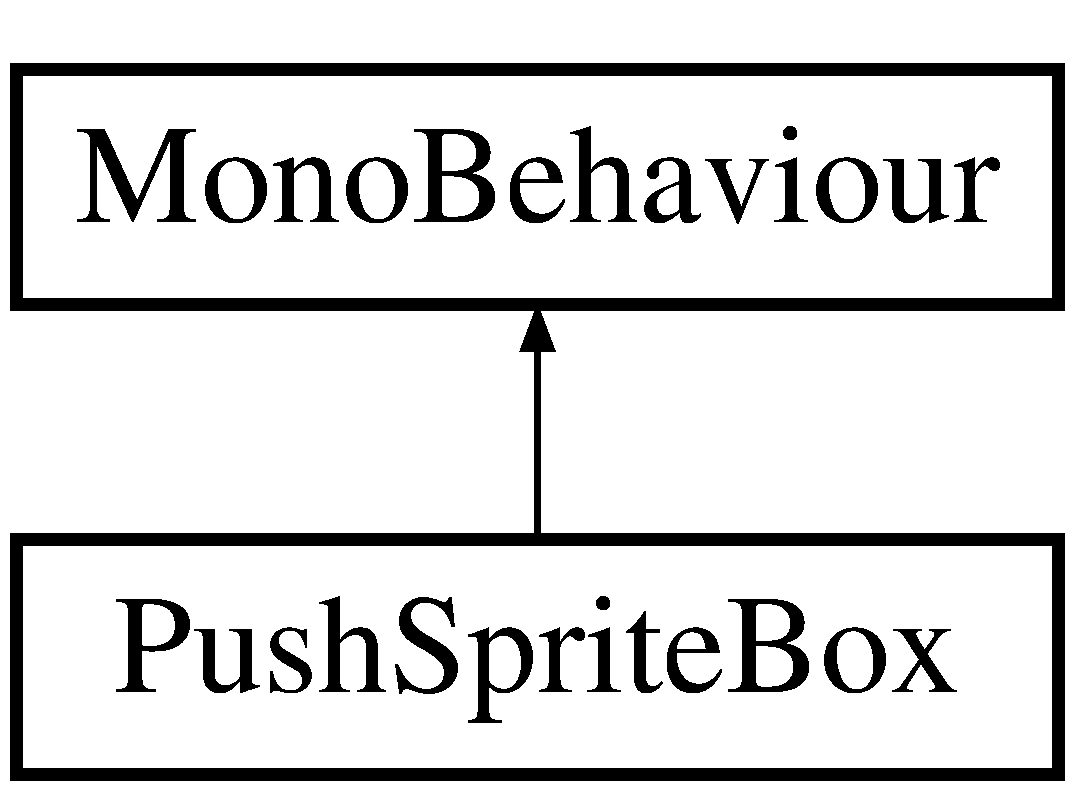
\includegraphics[height=2.000000cm]{class_push_sprite_box}
\end{center}
\end{figure}
\subsection*{Public Member Functions}
\begin{DoxyCompactItemize}
\item 
delegate void {\bfseries callback} ()\hypertarget{class_push_sprite_box_a3a2b1a81646210d8252c3a22cd0db4cb}{}\label{class_push_sprite_box_a3a2b1a81646210d8252c3a22cd0db4cb}

\item 
void \hyperlink{class_push_sprite_box_a9b11701a1b0d48f87ad0cf4b0a21f24f}{Init} (callback action=null)
\begin{DoxyCompactList}\small\item\em 初期化 \end{DoxyCompactList}\item 
void \hyperlink{class_push_sprite_box_abd97fb6c92c989a809df9e56b35cc249}{Set\+Call\+Back} (callback action)
\begin{DoxyCompactList}\small\item\em 離されたときに行う関数の代入 \end{DoxyCompactList}\item 
void \hyperlink{class_push_sprite_box_aa8766cf11790ecdd85a01eecb74171b0}{update} ()
\begin{DoxyCompactList}\small\item\em 更新 \end{DoxyCompactList}\end{DoxyCompactItemize}


\subsection{Detailed Description}
四角形の当たり判定を持ったスプライト 



\subsection{Member Function Documentation}
\index{Push\+Sprite\+Box@{Push\+Sprite\+Box}!Init@{Init}}
\index{Init@{Init}!Push\+Sprite\+Box@{Push\+Sprite\+Box}}
\subsubsection[{\texorpdfstring{Init(callback action=null)}{Init(callback action=null)}}]{\setlength{\rightskip}{0pt plus 5cm}void Push\+Sprite\+Box.\+Init (
\begin{DoxyParamCaption}
\item[{callback}]{action = {\ttfamily null}}
\end{DoxyParamCaption}
)\hspace{0.3cm}{\ttfamily [inline]}}\hypertarget{class_push_sprite_box_a9b11701a1b0d48f87ad0cf4b0a21f24f}{}\label{class_push_sprite_box_a9b11701a1b0d48f87ad0cf4b0a21f24f}


初期化 


\begin{DoxyParams}{Parameters}
{\em action} & \\
\hline
\end{DoxyParams}
\index{Push\+Sprite\+Box@{Push\+Sprite\+Box}!Set\+Call\+Back@{Set\+Call\+Back}}
\index{Set\+Call\+Back@{Set\+Call\+Back}!Push\+Sprite\+Box@{Push\+Sprite\+Box}}
\subsubsection[{\texorpdfstring{Set\+Call\+Back(callback action)}{SetCallBack(callback action)}}]{\setlength{\rightskip}{0pt plus 5cm}void Push\+Sprite\+Box.\+Set\+Call\+Back (
\begin{DoxyParamCaption}
\item[{callback}]{action}
\end{DoxyParamCaption}
)\hspace{0.3cm}{\ttfamily [inline]}}\hypertarget{class_push_sprite_box_abd97fb6c92c989a809df9e56b35cc249}{}\label{class_push_sprite_box_abd97fb6c92c989a809df9e56b35cc249}


離されたときに行う関数の代入 


\begin{DoxyParams}{Parameters}
{\em action} & \\
\hline
\end{DoxyParams}
\index{Push\+Sprite\+Box@{Push\+Sprite\+Box}!update@{update}}
\index{update@{update}!Push\+Sprite\+Box@{Push\+Sprite\+Box}}
\subsubsection[{\texorpdfstring{update()}{update()}}]{\setlength{\rightskip}{0pt plus 5cm}void Push\+Sprite\+Box.\+update (
\begin{DoxyParamCaption}
{}
\end{DoxyParamCaption}
)\hspace{0.3cm}{\ttfamily [inline]}}\hypertarget{class_push_sprite_box_aa8766cf11790ecdd85a01eecb74171b0}{}\label{class_push_sprite_box_aa8766cf11790ecdd85a01eecb74171b0}


更新 



The documentation for this class was generated from the following file\+:\begin{DoxyCompactItemize}
\item 
Scripts/\+Sprite/Push\+Sprite\+Box.\+cs\end{DoxyCompactItemize}

\hypertarget{class_push_sprite_circle}{}\section{Push\+Sprite\+Circle Class Reference}
\label{class_push_sprite_circle}\index{Push\+Sprite\+Circle@{Push\+Sprite\+Circle}}


四角形の当たり判定を持ったスプライト  


Inheritance diagram for Push\+Sprite\+Circle\+:\begin{figure}[H]
\begin{center}
\leavevmode
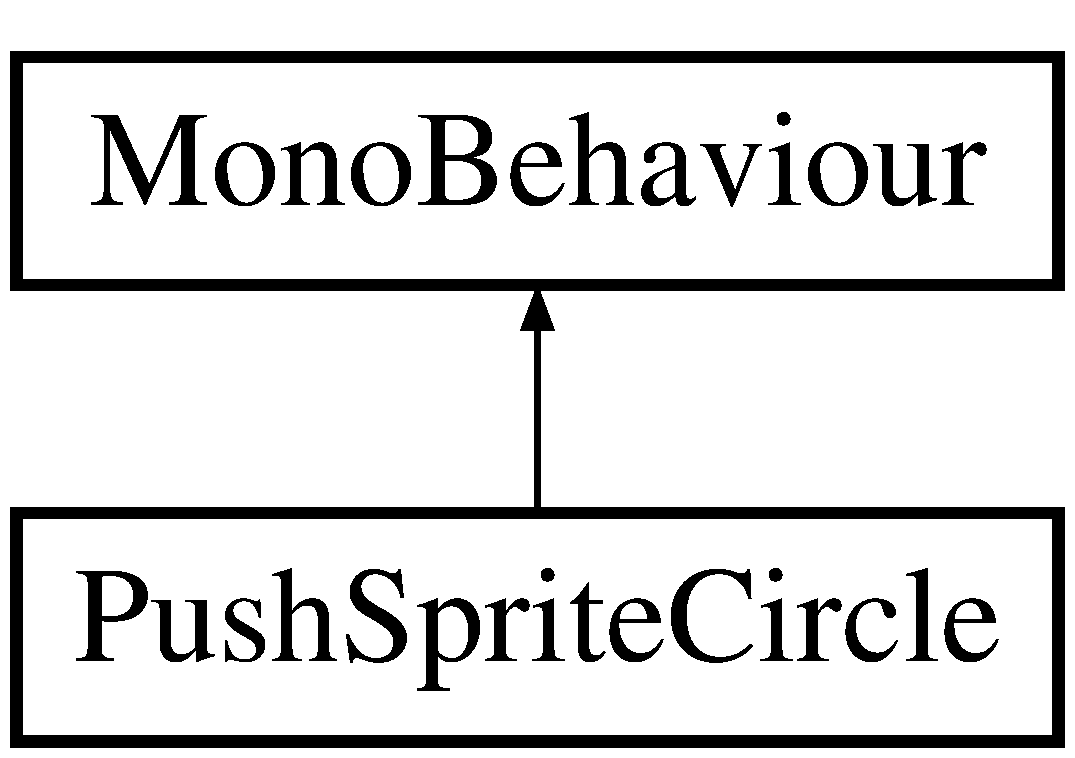
\includegraphics[height=2.000000cm]{class_push_sprite_circle}
\end{center}
\end{figure}
\subsection*{Public Member Functions}
\begin{DoxyCompactItemize}
\item 
delegate void {\bfseries callback} ()\hypertarget{class_push_sprite_circle_a19c5d07a0cf70f360b35a102cd5a7630}{}\label{class_push_sprite_circle_a19c5d07a0cf70f360b35a102cd5a7630}

\item 
void \hyperlink{class_push_sprite_circle_a016cadae34ba4c9445dffe122ca6592b}{Init} (callback action=null)
\begin{DoxyCompactList}\small\item\em 初期化 \end{DoxyCompactList}\item 
void \hyperlink{class_push_sprite_circle_a06299e5b04cea23a07ac0c5efe3037b6}{Set\+Call\+Back} (callback action)
\begin{DoxyCompactList}\small\item\em 離されたときに行う関数の代入 \end{DoxyCompactList}\item 
void \hyperlink{class_push_sprite_circle_a409c3ca3dd1c0f12ee4e9d3b0646bc85}{update} ()
\begin{DoxyCompactList}\small\item\em 更新 \end{DoxyCompactList}\end{DoxyCompactItemize}


\subsection{Detailed Description}
四角形の当たり判定を持ったスプライト 



\subsection{Member Function Documentation}
\index{Push\+Sprite\+Circle@{Push\+Sprite\+Circle}!Init@{Init}}
\index{Init@{Init}!Push\+Sprite\+Circle@{Push\+Sprite\+Circle}}
\subsubsection[{\texorpdfstring{Init(callback action=null)}{Init(callback action=null)}}]{\setlength{\rightskip}{0pt plus 5cm}void Push\+Sprite\+Circle.\+Init (
\begin{DoxyParamCaption}
\item[{callback}]{action = {\ttfamily null}}
\end{DoxyParamCaption}
)\hspace{0.3cm}{\ttfamily [inline]}}\hypertarget{class_push_sprite_circle_a016cadae34ba4c9445dffe122ca6592b}{}\label{class_push_sprite_circle_a016cadae34ba4c9445dffe122ca6592b}


初期化 


\begin{DoxyParams}{Parameters}
{\em action} & \\
\hline
\end{DoxyParams}
\index{Push\+Sprite\+Circle@{Push\+Sprite\+Circle}!Set\+Call\+Back@{Set\+Call\+Back}}
\index{Set\+Call\+Back@{Set\+Call\+Back}!Push\+Sprite\+Circle@{Push\+Sprite\+Circle}}
\subsubsection[{\texorpdfstring{Set\+Call\+Back(callback action)}{SetCallBack(callback action)}}]{\setlength{\rightskip}{0pt plus 5cm}void Push\+Sprite\+Circle.\+Set\+Call\+Back (
\begin{DoxyParamCaption}
\item[{callback}]{action}
\end{DoxyParamCaption}
)\hspace{0.3cm}{\ttfamily [inline]}}\hypertarget{class_push_sprite_circle_a06299e5b04cea23a07ac0c5efe3037b6}{}\label{class_push_sprite_circle_a06299e5b04cea23a07ac0c5efe3037b6}


離されたときに行う関数の代入 


\begin{DoxyParams}{Parameters}
{\em action} & \\
\hline
\end{DoxyParams}
\index{Push\+Sprite\+Circle@{Push\+Sprite\+Circle}!update@{update}}
\index{update@{update}!Push\+Sprite\+Circle@{Push\+Sprite\+Circle}}
\subsubsection[{\texorpdfstring{update()}{update()}}]{\setlength{\rightskip}{0pt plus 5cm}void Push\+Sprite\+Circle.\+update (
\begin{DoxyParamCaption}
{}
\end{DoxyParamCaption}
)\hspace{0.3cm}{\ttfamily [inline]}}\hypertarget{class_push_sprite_circle_a409c3ca3dd1c0f12ee4e9d3b0646bc85}{}\label{class_push_sprite_circle_a409c3ca3dd1c0f12ee4e9d3b0646bc85}


更新 



The documentation for this class was generated from the following file\+:\begin{DoxyCompactItemize}
\item 
Scripts/\+Sprite/Push\+Sprite\+Circle.\+cs\end{DoxyCompactItemize}

\hypertarget{class_rec_scene_controller}{}\section{Rec\+Scene\+Controller Class Reference}
\label{class_rec_scene_controller}\index{Rec\+Scene\+Controller@{Rec\+Scene\+Controller}}


記録用シーンのコントローラー  


Inheritance diagram for Rec\+Scene\+Controller\+:\begin{figure}[H]
\begin{center}
\leavevmode
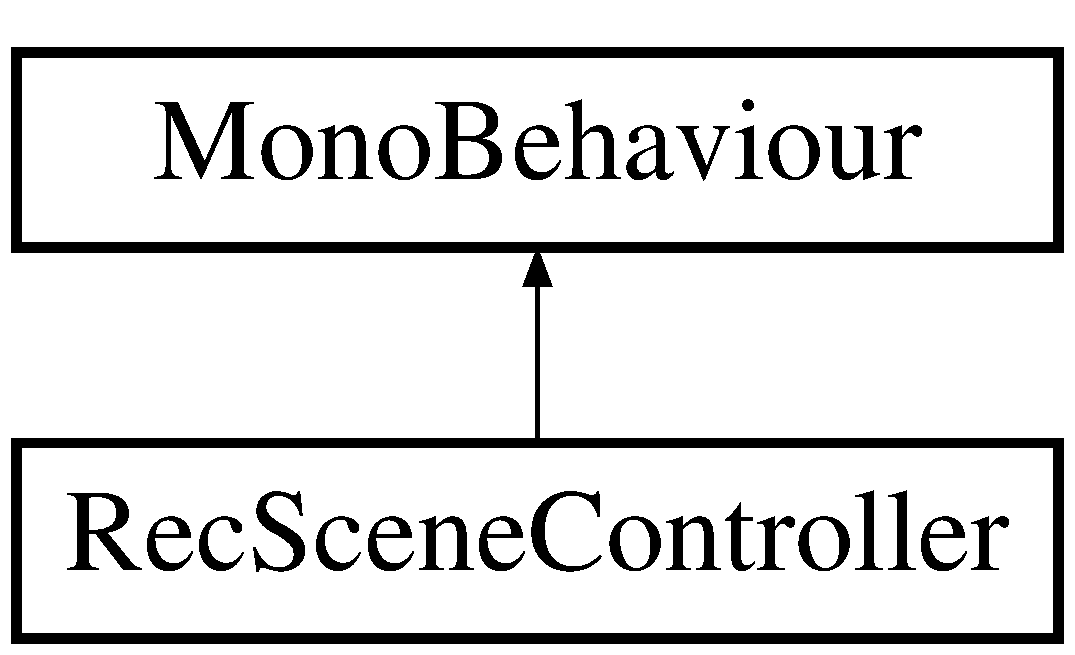
\includegraphics[height=2.000000cm]{class_rec_scene_controller}
\end{center}
\end{figure}
\subsection*{Public Member Functions}
\begin{DoxyCompactItemize}
\item 
void \hyperlink{class_rec_scene_controller_a01e8c4870a1506923a1960f62c15bf19}{Start\+Music} ()
\item 
void {\bfseries Start\+Test} ()\hypertarget{class_rec_scene_controller_a261af30fdd33ca0c5b6425fd2909aadf}{}\label{class_rec_scene_controller_a261af30fdd33ca0c5b6425fd2909aadf}

\end{DoxyCompactItemize}


\subsection{Detailed Description}
記録用シーンのコントローラー 



\subsection{Member Function Documentation}
\index{Rec\+Scene\+Controller@{Rec\+Scene\+Controller}!Start\+Music@{Start\+Music}}
\index{Start\+Music@{Start\+Music}!Rec\+Scene\+Controller@{Rec\+Scene\+Controller}}
\subsubsection[{\texorpdfstring{Start\+Music()}{StartMusic()}}]{\setlength{\rightskip}{0pt plus 5cm}void Rec\+Scene\+Controller.\+Start\+Music (
\begin{DoxyParamCaption}
{}
\end{DoxyParamCaption}
)\hspace{0.3cm}{\ttfamily [inline]}}\hypertarget{class_rec_scene_controller_a01e8c4870a1506923a1960f62c15bf19}{}\label{class_rec_scene_controller_a01e8c4870a1506923a1960f62c15bf19}






The documentation for this class was generated from the following file\+:\begin{DoxyCompactItemize}
\item 
Scripts/\+Scenes\+Controller/Rec\+Scene\+Controller.\+cs\end{DoxyCompactItemize}

\hypertarget{class_result_scene_controller}{}\section{Result\+Scene\+Controller Class Reference}
\label{class_result_scene_controller}\index{Result\+Scene\+Controller@{Result\+Scene\+Controller}}


リザルトシーンコントローラー  


Inheritance diagram for Result\+Scene\+Controller\+:\begin{figure}[H]
\begin{center}
\leavevmode
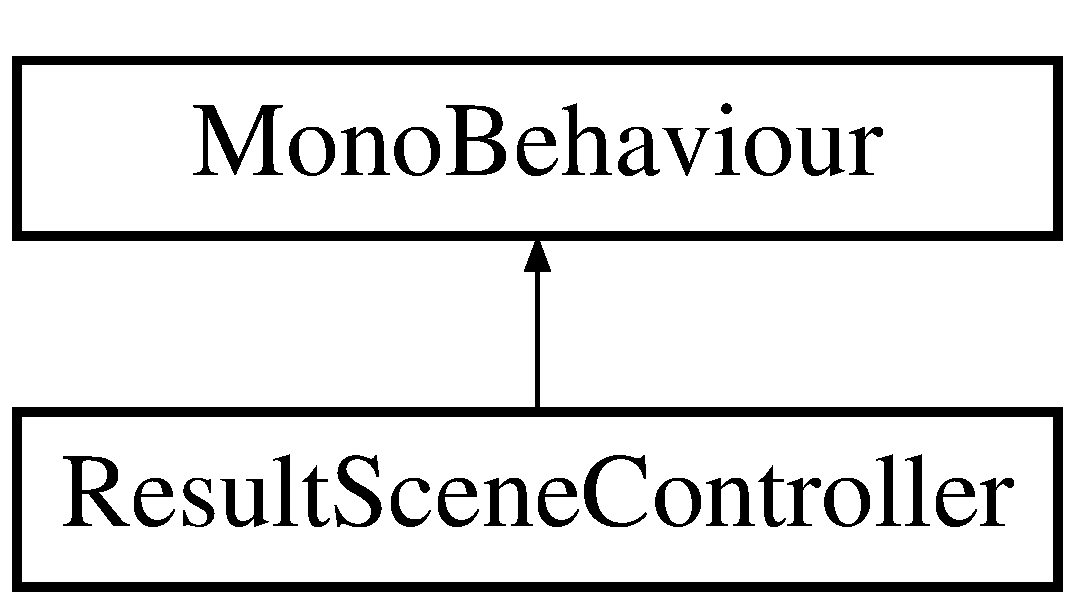
\includegraphics[height=2.000000cm]{class_result_scene_controller}
\end{center}
\end{figure}
\subsection*{Public Member Functions}
\begin{DoxyCompactItemize}
\item 
void \hyperlink{class_result_scene_controller_aa9865e524bbd9008a55c0b164240d3df}{Return\+Title} ()
\begin{DoxyCompactList}\small\item\em タイトルへ戻る \end{DoxyCompactList}\item 
void \hyperlink{class_result_scene_controller_a9e1acecea437e8c311b9ffb6bec77a6d}{Return\+Song\+Select} ()
\begin{DoxyCompactList}\small\item\em 曲選択へ戻る \end{DoxyCompactList}\end{DoxyCompactItemize}


\subsection{Detailed Description}
リザルトシーンコントローラー 



\subsection{Member Function Documentation}
\index{Result\+Scene\+Controller@{Result\+Scene\+Controller}!Return\+Song\+Select@{Return\+Song\+Select}}
\index{Return\+Song\+Select@{Return\+Song\+Select}!Result\+Scene\+Controller@{Result\+Scene\+Controller}}
\subsubsection[{\texorpdfstring{Return\+Song\+Select()}{ReturnSongSelect()}}]{\setlength{\rightskip}{0pt plus 5cm}void Result\+Scene\+Controller.\+Return\+Song\+Select (
\begin{DoxyParamCaption}
{}
\end{DoxyParamCaption}
)\hspace{0.3cm}{\ttfamily [inline]}}\hypertarget{class_result_scene_controller_a9e1acecea437e8c311b9ffb6bec77a6d}{}\label{class_result_scene_controller_a9e1acecea437e8c311b9ffb6bec77a6d}


曲選択へ戻る 

\index{Result\+Scene\+Controller@{Result\+Scene\+Controller}!Return\+Title@{Return\+Title}}
\index{Return\+Title@{Return\+Title}!Result\+Scene\+Controller@{Result\+Scene\+Controller}}
\subsubsection[{\texorpdfstring{Return\+Title()}{ReturnTitle()}}]{\setlength{\rightskip}{0pt plus 5cm}void Result\+Scene\+Controller.\+Return\+Title (
\begin{DoxyParamCaption}
{}
\end{DoxyParamCaption}
)\hspace{0.3cm}{\ttfamily [inline]}}\hypertarget{class_result_scene_controller_aa9865e524bbd9008a55c0b164240d3df}{}\label{class_result_scene_controller_aa9865e524bbd9008a55c0b164240d3df}


タイトルへ戻る 



The documentation for this class was generated from the following file\+:\begin{DoxyCompactItemize}
\item 
Scripts/\+Scenes\+Controller/Result\+Scene\+Controller.\+cs\end{DoxyCompactItemize}

\hypertarget{class_serialize_gizmos}{}\section{Serialize\+Gizmos Class Reference}
\label{class_serialize_gizmos}\index{Serialize\+Gizmos@{Serialize\+Gizmos}}
Inheritance diagram for Serialize\+Gizmos\+:\begin{figure}[H]
\begin{center}
\leavevmode
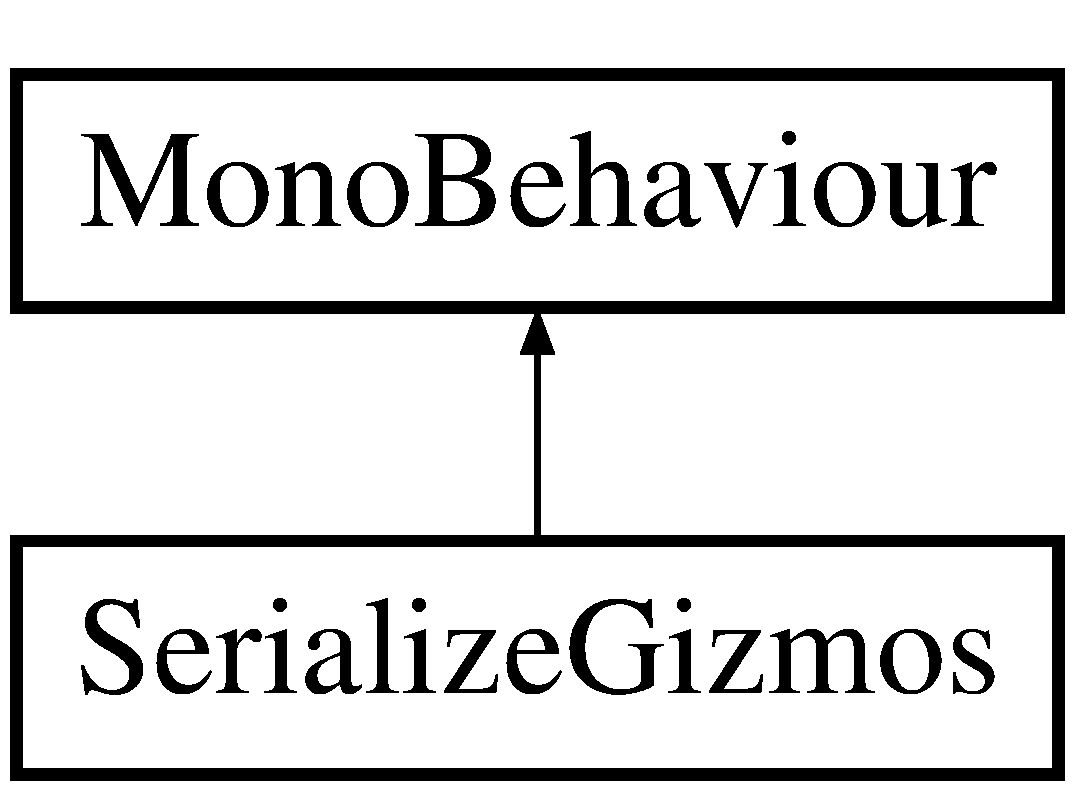
\includegraphics[height=2.000000cm]{class_serialize_gizmos}
\end{center}
\end{figure}


The documentation for this class was generated from the following file\+:\begin{DoxyCompactItemize}
\item 
Scripts/\+Serialize/Serialize\+Gizmos.\+cs\end{DoxyCompactItemize}

\hypertarget{class_serialize_line_gizmos}{}\section{Serialize\+Line\+Gizmos Class Reference}
\label{class_serialize_line_gizmos}\index{Serialize\+Line\+Gizmos@{Serialize\+Line\+Gizmos}}
Inheritance diagram for Serialize\+Line\+Gizmos\+:\begin{figure}[H]
\begin{center}
\leavevmode
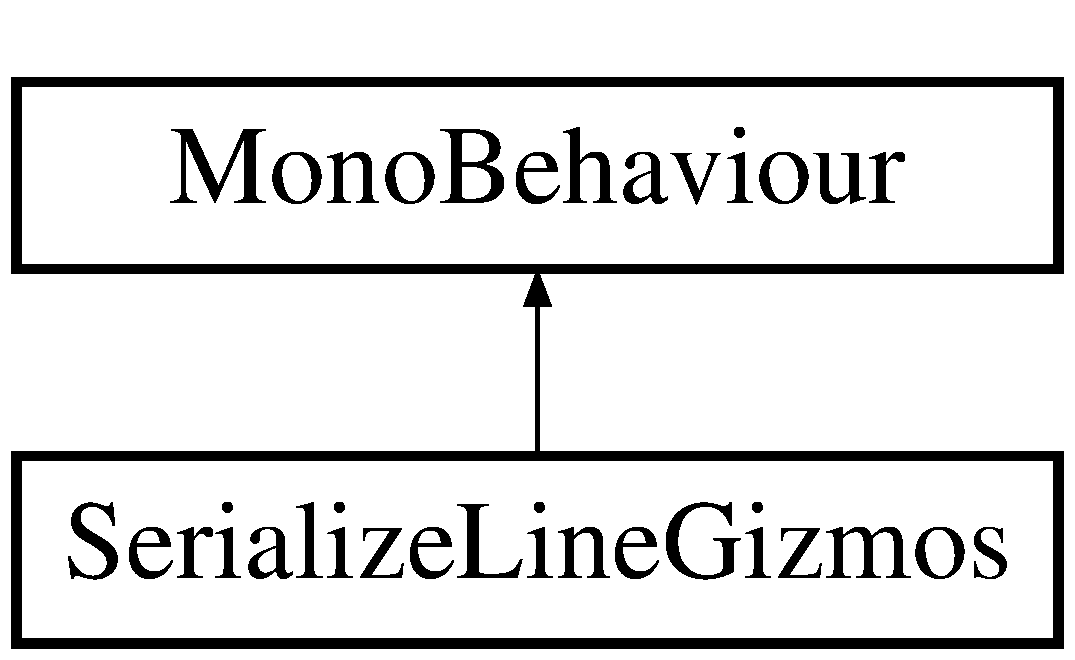
\includegraphics[height=2.000000cm]{class_serialize_line_gizmos}
\end{center}
\end{figure}


The documentation for this class was generated from the following file\+:\begin{DoxyCompactItemize}
\item 
Scripts/\+Serialize/Serialize\+Line\+Gizmos.\+cs\end{DoxyCompactItemize}

\hypertarget{class_single_notes}{}\section{Single\+Notes Class Reference}
\label{class_single_notes}\index{Single\+Notes@{Single\+Notes}}


単発ノーツ  


Inheritance diagram for Single\+Notes\+:\begin{figure}[H]
\begin{center}
\leavevmode
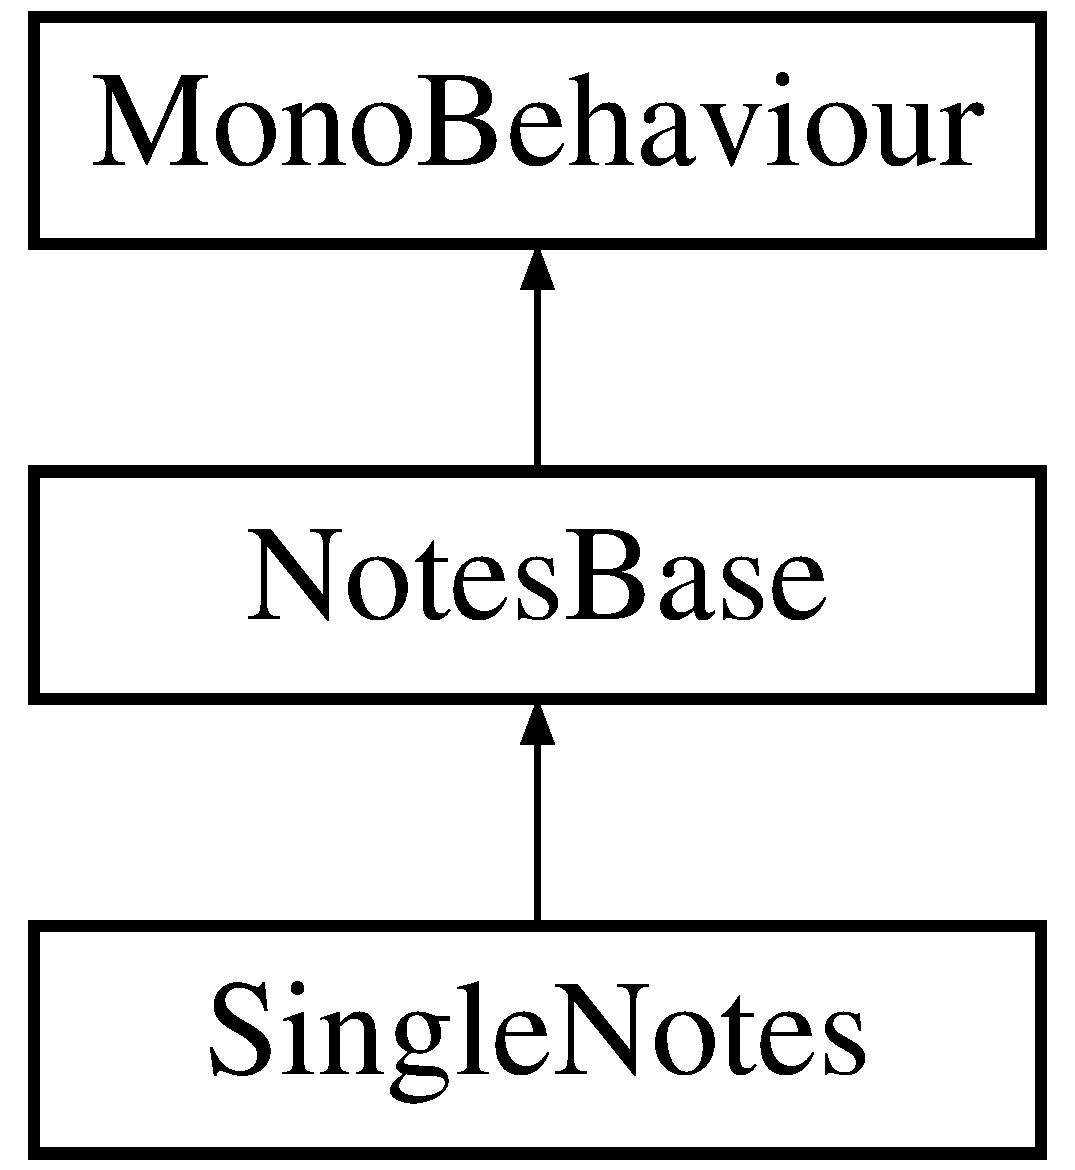
\includegraphics[height=3.000000cm]{class_single_notes}
\end{center}
\end{figure}
\subsection*{Public Member Functions}
\begin{DoxyCompactItemize}
\item 
override void {\bfseries Init} (int lane\+No, float down, float up)\hypertarget{class_single_notes_a06743f4372325fb1445d62eadc690446}{}\label{class_single_notes_a06743f4372325fb1445d62eadc690446}

\item 
override void \hyperlink{class_single_notes_ad845bd14668226c2edab7cc3aff1c575}{Move} ()
\begin{DoxyCompactList}\small\item\em ノーツの移動 \end{DoxyCompactList}\item 
void \hyperlink{class_single_notes_ac73c660a04161571760a41461ea7cf8b}{On\+Touch\+Down} ()
\begin{DoxyCompactList}\small\item\em 押したときの処理 \end{DoxyCompactList}\item 
void \hyperlink{class_single_notes_a1ac048470c51a39aae1aa48e1c2ab7fb}{Seed\+Fx\+Control} (float timming)
\begin{DoxyCompactList}\small\item\em 種火エフェクトの制御 \end{DoxyCompactList}\item 
override void \hyperlink{class_single_notes_a0ad7fbf218ce275691c094c42bda1103}{Miss} ()
\begin{DoxyCompactList}\small\item\em 失敗処理 \end{DoxyCompactList}\item 
override void \hyperlink{class_single_notes_a5e0ca4a12debb4cf39b7e4e24e0e0f7b}{Rec\+Init} (int lane\+No, float down, float up)
\begin{DoxyCompactList}\small\item\em 録画シーンの初期化 \end{DoxyCompactList}\end{DoxyCompactItemize}
\subsection*{Public Attributes}
\begin{DoxyCompactItemize}
\item 
const int {\bfseries ID} = 1\hypertarget{class_single_notes_ae0a33c1331d84f08785264179546422e}{}\label{class_single_notes_ae0a33c1331d84f08785264179546422e}

\end{DoxyCompactItemize}
\subsection*{Properties}
\begin{DoxyCompactItemize}
\item 
override bool \hyperlink{class_single_notes_ad8575a29920cd51c2f96a666f2ab18e0}{is\+Reset}\hspace{0.3cm}{\ttfamily  \mbox{[}get\mbox{]}}
\begin{DoxyCompactList}\small\item\em リセットフラグ \end{DoxyCompactList}\item 
override bool \hyperlink{class_single_notes_a4d6232399afbade1d1f3c7cbcb1f9b35}{is\+Miss}\hspace{0.3cm}{\ttfamily  \mbox{[}get\mbox{]}}
\begin{DoxyCompactList}\small\item\em ミスフラグ \end{DoxyCompactList}\end{DoxyCompactItemize}
\subsection*{Additional Inherited Members}


\subsection{Detailed Description}
単発ノーツ 



\subsection{Member Function Documentation}
\index{Single\+Notes@{Single\+Notes}!Miss@{Miss}}
\index{Miss@{Miss}!Single\+Notes@{Single\+Notes}}
\subsubsection[{\texorpdfstring{Miss()}{Miss()}}]{\setlength{\rightskip}{0pt plus 5cm}override void Single\+Notes.\+Miss (
\begin{DoxyParamCaption}
{}
\end{DoxyParamCaption}
)\hspace{0.3cm}{\ttfamily [inline]}, {\ttfamily [virtual]}}\hypertarget{class_single_notes_a0ad7fbf218ce275691c094c42bda1103}{}\label{class_single_notes_a0ad7fbf218ce275691c094c42bda1103}


失敗処理 



Reimplemented from \hyperlink{class_notes_base}{Notes\+Base}.

\index{Single\+Notes@{Single\+Notes}!Move@{Move}}
\index{Move@{Move}!Single\+Notes@{Single\+Notes}}
\subsubsection[{\texorpdfstring{Move()}{Move()}}]{\setlength{\rightskip}{0pt plus 5cm}override void Single\+Notes.\+Move (
\begin{DoxyParamCaption}
{}
\end{DoxyParamCaption}
)\hspace{0.3cm}{\ttfamily [inline]}, {\ttfamily [virtual]}}\hypertarget{class_single_notes_ad845bd14668226c2edab7cc3aff1c575}{}\label{class_single_notes_ad845bd14668226c2edab7cc3aff1c575}


ノーツの移動 



Reimplemented from \hyperlink{class_notes_base}{Notes\+Base}.

\index{Single\+Notes@{Single\+Notes}!On\+Touch\+Down@{On\+Touch\+Down}}
\index{On\+Touch\+Down@{On\+Touch\+Down}!Single\+Notes@{Single\+Notes}}
\subsubsection[{\texorpdfstring{On\+Touch\+Down()}{OnTouchDown()}}]{\setlength{\rightskip}{0pt plus 5cm}void Single\+Notes.\+On\+Touch\+Down (
\begin{DoxyParamCaption}
{}
\end{DoxyParamCaption}
)\hspace{0.3cm}{\ttfamily [inline]}}\hypertarget{class_single_notes_ac73c660a04161571760a41461ea7cf8b}{}\label{class_single_notes_ac73c660a04161571760a41461ea7cf8b}


押したときの処理 

\index{Single\+Notes@{Single\+Notes}!Rec\+Init@{Rec\+Init}}
\index{Rec\+Init@{Rec\+Init}!Single\+Notes@{Single\+Notes}}
\subsubsection[{\texorpdfstring{Rec\+Init(int lane\+No, float down, float up)}{RecInit(int laneNo, float down, float up)}}]{\setlength{\rightskip}{0pt plus 5cm}override void Single\+Notes.\+Rec\+Init (
\begin{DoxyParamCaption}
\item[{int}]{lane\+No, }
\item[{float}]{down, }
\item[{float}]{up}
\end{DoxyParamCaption}
)\hspace{0.3cm}{\ttfamily [inline]}, {\ttfamily [virtual]}}\hypertarget{class_single_notes_a5e0ca4a12debb4cf39b7e4e24e0e0f7b}{}\label{class_single_notes_a5e0ca4a12debb4cf39b7e4e24e0e0f7b}


録画シーンの初期化 



Reimplemented from \hyperlink{class_notes_base}{Notes\+Base}.

\index{Single\+Notes@{Single\+Notes}!Seed\+Fx\+Control@{Seed\+Fx\+Control}}
\index{Seed\+Fx\+Control@{Seed\+Fx\+Control}!Single\+Notes@{Single\+Notes}}
\subsubsection[{\texorpdfstring{Seed\+Fx\+Control(float timming)}{SeedFxControl(float timming)}}]{\setlength{\rightskip}{0pt plus 5cm}void Single\+Notes.\+Seed\+Fx\+Control (
\begin{DoxyParamCaption}
\item[{float}]{timming}
\end{DoxyParamCaption}
)\hspace{0.3cm}{\ttfamily [inline]}}\hypertarget{class_single_notes_a1ac048470c51a39aae1aa48e1c2ab7fb}{}\label{class_single_notes_a1ac048470c51a39aae1aa48e1c2ab7fb}


種火エフェクトの制御 



\subsection{Property Documentation}
\index{Single\+Notes@{Single\+Notes}!is\+Miss@{is\+Miss}}
\index{is\+Miss@{is\+Miss}!Single\+Notes@{Single\+Notes}}
\subsubsection[{\texorpdfstring{is\+Miss}{isMiss}}]{\setlength{\rightskip}{0pt plus 5cm}override bool Single\+Notes.\+is\+Miss\hspace{0.3cm}{\ttfamily [get]}}\hypertarget{class_single_notes_a4d6232399afbade1d1f3c7cbcb1f9b35}{}\label{class_single_notes_a4d6232399afbade1d1f3c7cbcb1f9b35}


ミスフラグ 

\index{Single\+Notes@{Single\+Notes}!is\+Reset@{is\+Reset}}
\index{is\+Reset@{is\+Reset}!Single\+Notes@{Single\+Notes}}
\subsubsection[{\texorpdfstring{is\+Reset}{isReset}}]{\setlength{\rightskip}{0pt plus 5cm}override bool Single\+Notes.\+is\+Reset\hspace{0.3cm}{\ttfamily [get]}}\hypertarget{class_single_notes_ad8575a29920cd51c2f96a666f2ab18e0}{}\label{class_single_notes_ad8575a29920cd51c2f96a666f2ab18e0}


リセットフラグ 



The documentation for this class was generated from the following file\+:\begin{DoxyCompactItemize}
\item 
Scripts/\+Notes/Single\+Notes.\+cs\end{DoxyCompactItemize}

\hypertarget{class_single_notes_big_fire_works_pool}{}\section{Single\+Notes\+Big\+Fire\+Works\+Pool Class Reference}
\label{class_single_notes_big_fire_works_pool}\index{Single\+Notes\+Big\+Fire\+Works\+Pool@{Single\+Notes\+Big\+Fire\+Works\+Pool}}
Inheritance diagram for Single\+Notes\+Big\+Fire\+Works\+Pool\+:\begin{figure}[H]
\begin{center}
\leavevmode
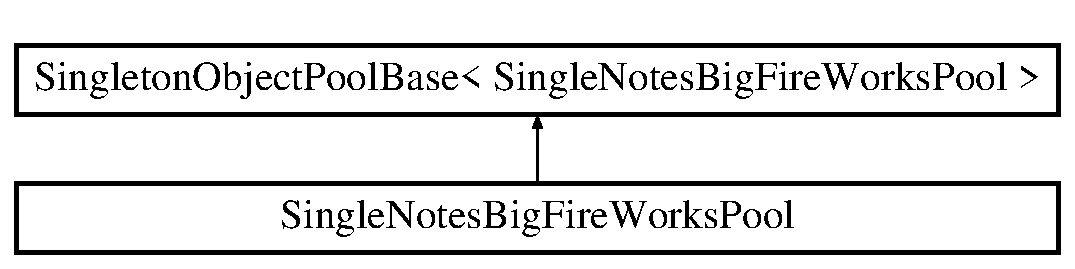
\includegraphics[height=2.000000cm]{class_single_notes_big_fire_works_pool}
\end{center}
\end{figure}
\subsection*{Public Member Functions}
\begin{DoxyCompactItemize}
\item 
void {\bfseries Run} (Vector3 pos)\hypertarget{class_single_notes_big_fire_works_pool_af8554599e8fb1d2f6e44d01af20b7b60}{}\label{class_single_notes_big_fire_works_pool_af8554599e8fb1d2f6e44d01af20b7b60}

\end{DoxyCompactItemize}
\subsection*{Additional Inherited Members}


The documentation for this class was generated from the following file\+:\begin{DoxyCompactItemize}
\item 
Scripts/\+Object\+Pool/Single\+Notes\+Big\+Fire\+Works\+Pool.\+cs\end{DoxyCompactItemize}

\hypertarget{class_single_notes_pools}{}\section{Single\+Notes\+Pools Class Reference}
\label{class_single_notes_pools}\index{Single\+Notes\+Pools@{Single\+Notes\+Pools}}
Inheritance diagram for Single\+Notes\+Pools\+:\begin{figure}[H]
\begin{center}
\leavevmode
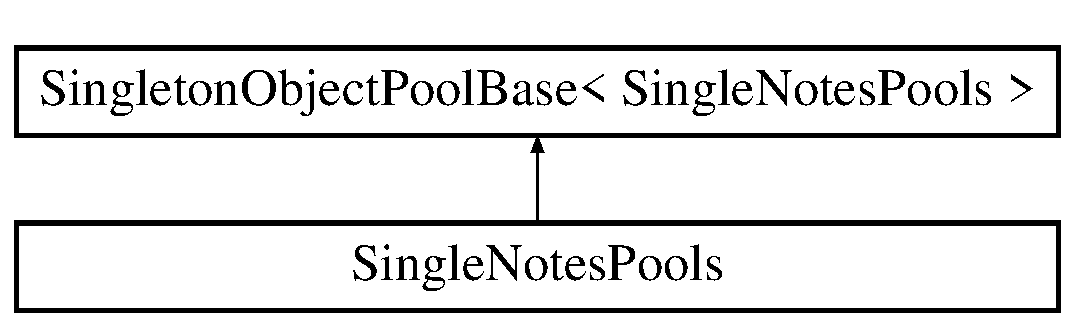
\includegraphics[height=2.000000cm]{class_single_notes_pools}
\end{center}
\end{figure}
\subsection*{Additional Inherited Members}


The documentation for this class was generated from the following file\+:\begin{DoxyCompactItemize}
\item 
Scripts/\+Object\+Pool/Single\+Notes\+Pools.\+cs\end{DoxyCompactItemize}

\hypertarget{class_single_notes_small_fire_works_pool}{}\section{Single\+Notes\+Small\+Fire\+Works\+Pool Class Reference}
\label{class_single_notes_small_fire_works_pool}\index{Single\+Notes\+Small\+Fire\+Works\+Pool@{Single\+Notes\+Small\+Fire\+Works\+Pool}}
Inheritance diagram for Single\+Notes\+Small\+Fire\+Works\+Pool\+:\begin{figure}[H]
\begin{center}
\leavevmode
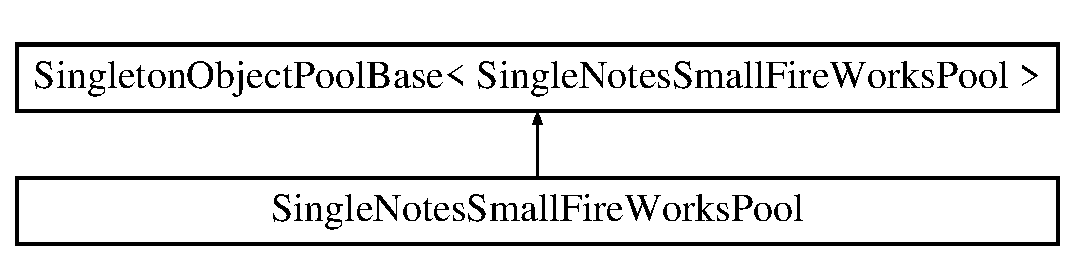
\includegraphics[height=2.000000cm]{class_single_notes_small_fire_works_pool}
\end{center}
\end{figure}
\subsection*{Public Member Functions}
\begin{DoxyCompactItemize}
\item 
void {\bfseries Run} (Vector3 pos)\hypertarget{class_single_notes_small_fire_works_pool_abb102bd0e2551b7e2b4f94d3c8494aa8}{}\label{class_single_notes_small_fire_works_pool_abb102bd0e2551b7e2b4f94d3c8494aa8}

\end{DoxyCompactItemize}
\subsection*{Additional Inherited Members}


The documentation for this class was generated from the following file\+:\begin{DoxyCompactItemize}
\item 
Scripts/\+Object\+Pool/Single\+Notes\+Small\+Fire\+Works\+Pool.\+cs\end{DoxyCompactItemize}

\hypertarget{class_singleton_base}{}\section{Singleton\+Base$<$ T $>$ Class Template Reference}
\label{class_singleton_base}\index{Singleton\+Base$<$ T $>$@{Singleton\+Base$<$ T $>$}}
\subsection*{Static Public Member Functions}
\begin{DoxyCompactItemize}
\item 
static void {\bfseries Remove\+Reference} ()\hypertarget{class_singleton_base_a315f2c75cec6af37d9db6ead590b9bf9}{}\label{class_singleton_base_a315f2c75cec6af37d9db6ead590b9bf9}

\item 
static void {\bfseries Create\+Reference} ()\hypertarget{class_singleton_base_a15797370a65507e0a722da0b57b3f4b2}{}\label{class_singleton_base_a15797370a65507e0a722da0b57b3f4b2}

\end{DoxyCompactItemize}
\subsection*{Properties}
\begin{DoxyCompactItemize}
\item 
static T {\bfseries Instance}\hspace{0.3cm}{\ttfamily  \mbox{[}get\mbox{]}}\hypertarget{class_singleton_base_aa726d096ab07668698600ad2a6c1744a}{}\label{class_singleton_base_aa726d096ab07668698600ad2a6c1744a}

\end{DoxyCompactItemize}


The documentation for this class was generated from the following file\+:\begin{DoxyCompactItemize}
\item 
Scripts/\+Base/Singleton\+Base.\+cs\end{DoxyCompactItemize}

\hypertarget{class_singleton_mono_behaviour}{}\section{Singleton\+Mono\+Behaviour$<$ T $>$ Class Template Reference}
\label{class_singleton_mono_behaviour}\index{Singleton\+Mono\+Behaviour$<$ T $>$@{Singleton\+Mono\+Behaviour$<$ T $>$}}


シングルトンの基底クラス テンプレートに近い  


Inheritance diagram for Singleton\+Mono\+Behaviour$<$ T $>$\+:\begin{figure}[H]
\begin{center}
\leavevmode
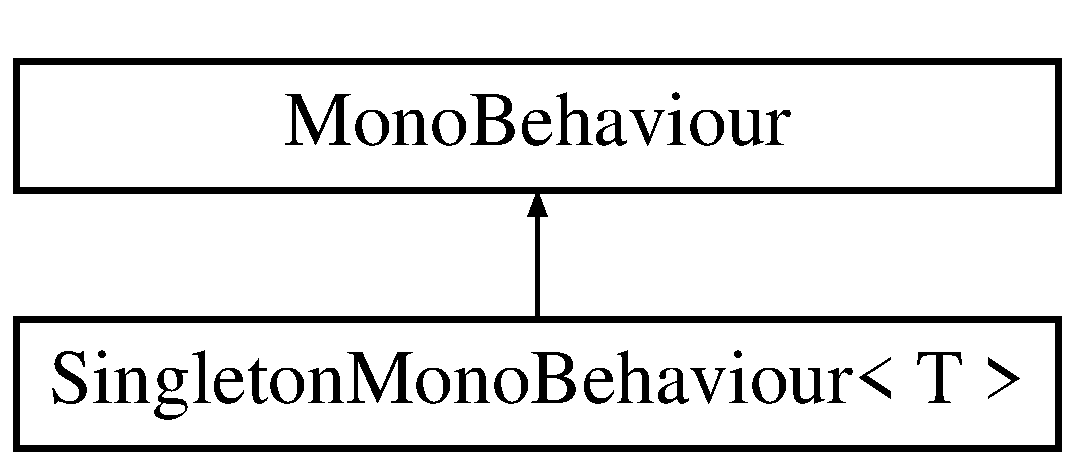
\includegraphics[height=2.000000cm]{class_singleton_mono_behaviour}
\end{center}
\end{figure}
\subsection*{Properties}
\begin{DoxyCompactItemize}
\item 
static T {\bfseries Instance}\hspace{0.3cm}{\ttfamily  \mbox{[}get\mbox{]}}\hypertarget{class_singleton_mono_behaviour_a2e1b552aa6b4ed45e1039c0d3d31a05a}{}\label{class_singleton_mono_behaviour_a2e1b552aa6b4ed45e1039c0d3d31a05a}

\end{DoxyCompactItemize}


\subsection{Detailed Description}
シングルトンの基底クラス テンプレートに近い 


\begin{DoxyTemplParams}{Template Parameters}
{\em T} & \\
\hline
\end{DoxyTemplParams}
\begin{Desc}
\item[Type Constraints]\begin{description}
\item[{\em T} : {\em Mono\+Behaviour}]\end{description}
\end{Desc}


The documentation for this class was generated from the following file\+:\begin{DoxyCompactItemize}
\item 
Scripts/\+Base/Singleton\+Mono\+Behaviour.\+cs\end{DoxyCompactItemize}

\hypertarget{class_singleton_object_pool_base}{}\section{Singleton\+Object\+Pool\+Base$<$ T $>$ Class Template Reference}
\label{class_singleton_object_pool_base}\index{Singleton\+Object\+Pool\+Base$<$ T $>$@{Singleton\+Object\+Pool\+Base$<$ T $>$}}


 


Inheritance diagram for Singleton\+Object\+Pool\+Base$<$ T $>$\+:\begin{figure}[H]
\begin{center}
\leavevmode
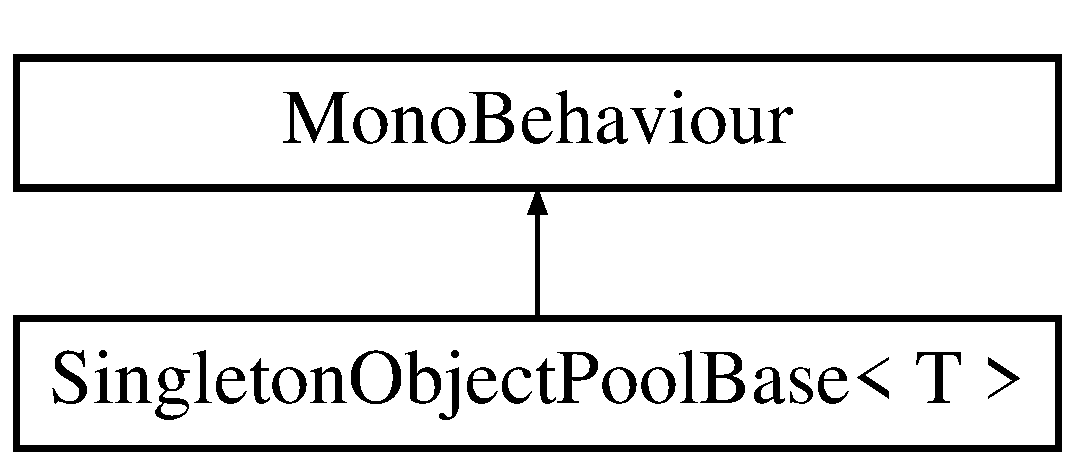
\includegraphics[height=2.000000cm]{class_singleton_object_pool_base}
\end{center}
\end{figure}
\subsection*{Public Member Functions}
\begin{DoxyCompactItemize}
\item 
virtual void \hyperlink{class_singleton_object_pool_base_ac7911635f1fff2562f4e0fe260f8addb}{Initialize} ()
\begin{DoxyCompactList}\small\item\em 初期化 (ここではプール生成後に\+Set\+Active(false)を呼び出している) \end{DoxyCompactList}\item 
virtual void \hyperlink{class_singleton_object_pool_base_a243b2d0a5b80b5b2e479dc2c5beeb079}{Renewal} ()
\begin{DoxyCompactList}\small\item\em リストを新しくする \end{DoxyCompactList}\item 
virtual Game\+Object \hyperlink{class_singleton_object_pool_base_a1957d69d05289232b43cb8e24a1bc648}{Get\+Object} ()
\begin{DoxyCompactList}\small\item\em プールオブジェクトの取得 \end{DoxyCompactList}\end{DoxyCompactItemize}
\subsection*{Protected Member Functions}
\begin{DoxyCompactItemize}
\item 
void \hyperlink{class_singleton_object_pool_base_a31f837eb2f5bafd9e7b3b275f39329a6}{Create\+Pool} ()
\begin{DoxyCompactList}\small\item\em プールの生成 \end{DoxyCompactList}\end{DoxyCompactItemize}
\subsection*{Protected Attributes}
\begin{DoxyCompactItemize}
\item 
Game\+Object {\bfseries pool\+Object}\hypertarget{class_singleton_object_pool_base_a2a95e2e9ebbee11165f3f13b31b866ec}{}\label{class_singleton_object_pool_base_a2a95e2e9ebbee11165f3f13b31b866ec}

\item 
int {\bfseries pool\+Num}\hypertarget{class_singleton_object_pool_base_a876763d012019bbd0beee30e65df03af}{}\label{class_singleton_object_pool_base_a876763d012019bbd0beee30e65df03af}

\item 
List$<$ Game\+Object $>$ {\bfseries pool\+List}\hypertarget{class_singleton_object_pool_base_a877383a71dc7b4327c5462e7d5807ded}{}\label{class_singleton_object_pool_base_a877383a71dc7b4327c5462e7d5807ded}

\end{DoxyCompactItemize}
\subsection*{Properties}
\begin{DoxyCompactItemize}
\item 
static T {\bfseries Instance}\hspace{0.3cm}{\ttfamily  \mbox{[}get\mbox{]}}\hypertarget{class_singleton_object_pool_base_ab906d15c93813acbd1ac4f58da2c9b6a}{}\label{class_singleton_object_pool_base_ab906d15c93813acbd1ac4f58da2c9b6a}

\end{DoxyCompactItemize}


\subsection{Detailed Description}



\begin{DoxyTemplParams}{Template Parameters}
{\em T} & \\
\hline
\end{DoxyTemplParams}
\begin{Desc}
\item[Type Constraints]\begin{description}
\item[{\em T} : {\em Mono\+Behaviour}]\end{description}
\end{Desc}


\subsection{Member Function Documentation}
\index{Singleton\+Object\+Pool\+Base@{Singleton\+Object\+Pool\+Base}!Create\+Pool@{Create\+Pool}}
\index{Create\+Pool@{Create\+Pool}!Singleton\+Object\+Pool\+Base@{Singleton\+Object\+Pool\+Base}}
\subsubsection[{\texorpdfstring{Create\+Pool()}{CreatePool()}}]{\setlength{\rightskip}{0pt plus 5cm}void {\bf Singleton\+Object\+Pool\+Base}$<$ T $>$.Create\+Pool (
\begin{DoxyParamCaption}
{}
\end{DoxyParamCaption}
)\hspace{0.3cm}{\ttfamily [inline]}, {\ttfamily [protected]}}\hypertarget{class_singleton_object_pool_base_a31f837eb2f5bafd9e7b3b275f39329a6}{}\label{class_singleton_object_pool_base_a31f837eb2f5bafd9e7b3b275f39329a6}


プールの生成 

\index{Singleton\+Object\+Pool\+Base@{Singleton\+Object\+Pool\+Base}!Get\+Object@{Get\+Object}}
\index{Get\+Object@{Get\+Object}!Singleton\+Object\+Pool\+Base@{Singleton\+Object\+Pool\+Base}}
\subsubsection[{\texorpdfstring{Get\+Object()}{GetObject()}}]{\setlength{\rightskip}{0pt plus 5cm}virtual Game\+Object {\bf Singleton\+Object\+Pool\+Base}$<$ T $>$.Get\+Object (
\begin{DoxyParamCaption}
{}
\end{DoxyParamCaption}
)\hspace{0.3cm}{\ttfamily [inline]}, {\ttfamily [virtual]}}\hypertarget{class_singleton_object_pool_base_a1957d69d05289232b43cb8e24a1bc648}{}\label{class_singleton_object_pool_base_a1957d69d05289232b43cb8e24a1bc648}


プールオブジェクトの取得 

\begin{DoxyReturn}{Returns}

\end{DoxyReturn}
\index{Singleton\+Object\+Pool\+Base@{Singleton\+Object\+Pool\+Base}!Initialize@{Initialize}}
\index{Initialize@{Initialize}!Singleton\+Object\+Pool\+Base@{Singleton\+Object\+Pool\+Base}}
\subsubsection[{\texorpdfstring{Initialize()}{Initialize()}}]{\setlength{\rightskip}{0pt plus 5cm}virtual void {\bf Singleton\+Object\+Pool\+Base}$<$ T $>$.Initialize (
\begin{DoxyParamCaption}
{}
\end{DoxyParamCaption}
)\hspace{0.3cm}{\ttfamily [inline]}, {\ttfamily [virtual]}}\hypertarget{class_singleton_object_pool_base_ac7911635f1fff2562f4e0fe260f8addb}{}\label{class_singleton_object_pool_base_ac7911635f1fff2562f4e0fe260f8addb}


初期化 (ここではプール生成後に\+Set\+Active(false)を呼び出している) 

\index{Singleton\+Object\+Pool\+Base@{Singleton\+Object\+Pool\+Base}!Renewal@{Renewal}}
\index{Renewal@{Renewal}!Singleton\+Object\+Pool\+Base@{Singleton\+Object\+Pool\+Base}}
\subsubsection[{\texorpdfstring{Renewal()}{Renewal()}}]{\setlength{\rightskip}{0pt plus 5cm}virtual void {\bf Singleton\+Object\+Pool\+Base}$<$ T $>$.Renewal (
\begin{DoxyParamCaption}
{}
\end{DoxyParamCaption}
)\hspace{0.3cm}{\ttfamily [inline]}, {\ttfamily [virtual]}}\hypertarget{class_singleton_object_pool_base_a243b2d0a5b80b5b2e479dc2c5beeb079}{}\label{class_singleton_object_pool_base_a243b2d0a5b80b5b2e479dc2c5beeb079}


リストを新しくする 



The documentation for this class was generated from the following file\+:\begin{DoxyCompactItemize}
\item 
Scripts/\+Base/Singleton\+Object\+Pool\+Base.\+cs\end{DoxyCompactItemize}

\hypertarget{class_song_select_scene_controller}{}\section{Song\+Select\+Scene\+Controller Class Reference}
\label{class_song_select_scene_controller}\index{Song\+Select\+Scene\+Controller@{Song\+Select\+Scene\+Controller}}


曲選択画面  


Inheritance diagram for Song\+Select\+Scene\+Controller\+:\begin{figure}[H]
\begin{center}
\leavevmode
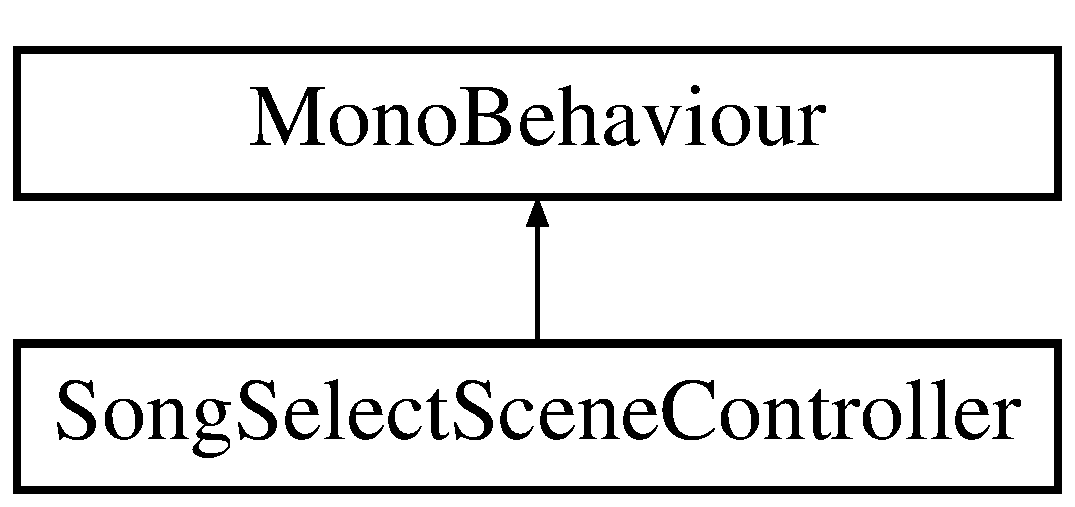
\includegraphics[height=2.000000cm]{class_song_select_scene_controller}
\end{center}
\end{figure}
\subsection*{Public Member Functions}
\begin{DoxyCompactItemize}
\item 
void \hyperlink{class_song_select_scene_controller_acb99166110cfceb7b53d679e1b4c16c2}{Trans\+Title\+Scene} ()
\begin{DoxyCompactList}\small\item\em タイトルシーンへ遷移 \end{DoxyCompactList}\item 
void \hyperlink{class_song_select_scene_controller_a2dcb0fe8a6c4196d78ed72800f3e8002}{Select\+Easy} ()
\begin{DoxyCompactList}\small\item\em \char`\"{}易\char`\"{}選択 \end{DoxyCompactList}\item 
void \hyperlink{class_song_select_scene_controller_a2e985edd5a3eea1aff475672a73b9c92}{Select\+Normal} ()
\begin{DoxyCompactList}\small\item\em \char`\"{}普\char`\"{}選択 \end{DoxyCompactList}\item 
void \hyperlink{class_song_select_scene_controller_ac066361fea8a0bf076e5d6e1859552ba}{Select\+Hard} ()
\begin{DoxyCompactList}\small\item\em \char`\"{}難\char`\"{}選択 \end{DoxyCompactList}\item 
void \hyperlink{class_song_select_scene_controller_ac5375256b9e14575e4a2908d87e3e5d3}{Play} ()
\begin{DoxyCompactList}\small\item\em ゲームプレイ \end{DoxyCompactList}\item 
void \hyperlink{class_song_select_scene_controller_ac7ac17097083308091146568ac0cdefa}{Start\+Open\+Option} ()
\begin{DoxyCompactList}\small\item\em オプションを開く \end{DoxyCompactList}\item 
void \hyperlink{class_song_select_scene_controller_a82e77f9bc2397d91fa82b2e8c200b187}{Start\+Close\+Option} ()
\begin{DoxyCompactList}\small\item\em オプションを閉じる \end{DoxyCompactList}\end{DoxyCompactItemize}


\subsection{Detailed Description}
曲選択画面 



\subsection{Member Function Documentation}
\index{Song\+Select\+Scene\+Controller@{Song\+Select\+Scene\+Controller}!Play@{Play}}
\index{Play@{Play}!Song\+Select\+Scene\+Controller@{Song\+Select\+Scene\+Controller}}
\subsubsection[{\texorpdfstring{Play()}{Play()}}]{\setlength{\rightskip}{0pt plus 5cm}void Song\+Select\+Scene\+Controller.\+Play (
\begin{DoxyParamCaption}
{}
\end{DoxyParamCaption}
)\hspace{0.3cm}{\ttfamily [inline]}}\hypertarget{class_song_select_scene_controller_ac5375256b9e14575e4a2908d87e3e5d3}{}\label{class_song_select_scene_controller_ac5375256b9e14575e4a2908d87e3e5d3}


ゲームプレイ 

\index{Song\+Select\+Scene\+Controller@{Song\+Select\+Scene\+Controller}!Select\+Easy@{Select\+Easy}}
\index{Select\+Easy@{Select\+Easy}!Song\+Select\+Scene\+Controller@{Song\+Select\+Scene\+Controller}}
\subsubsection[{\texorpdfstring{Select\+Easy()}{SelectEasy()}}]{\setlength{\rightskip}{0pt plus 5cm}void Song\+Select\+Scene\+Controller.\+Select\+Easy (
\begin{DoxyParamCaption}
{}
\end{DoxyParamCaption}
)\hspace{0.3cm}{\ttfamily [inline]}}\hypertarget{class_song_select_scene_controller_a2dcb0fe8a6c4196d78ed72800f3e8002}{}\label{class_song_select_scene_controller_a2dcb0fe8a6c4196d78ed72800f3e8002}


\char`\"{}易\char`\"{}選択 

\index{Song\+Select\+Scene\+Controller@{Song\+Select\+Scene\+Controller}!Select\+Hard@{Select\+Hard}}
\index{Select\+Hard@{Select\+Hard}!Song\+Select\+Scene\+Controller@{Song\+Select\+Scene\+Controller}}
\subsubsection[{\texorpdfstring{Select\+Hard()}{SelectHard()}}]{\setlength{\rightskip}{0pt plus 5cm}void Song\+Select\+Scene\+Controller.\+Select\+Hard (
\begin{DoxyParamCaption}
{}
\end{DoxyParamCaption}
)\hspace{0.3cm}{\ttfamily [inline]}}\hypertarget{class_song_select_scene_controller_ac066361fea8a0bf076e5d6e1859552ba}{}\label{class_song_select_scene_controller_ac066361fea8a0bf076e5d6e1859552ba}


\char`\"{}難\char`\"{}選択 

\index{Song\+Select\+Scene\+Controller@{Song\+Select\+Scene\+Controller}!Select\+Normal@{Select\+Normal}}
\index{Select\+Normal@{Select\+Normal}!Song\+Select\+Scene\+Controller@{Song\+Select\+Scene\+Controller}}
\subsubsection[{\texorpdfstring{Select\+Normal()}{SelectNormal()}}]{\setlength{\rightskip}{0pt plus 5cm}void Song\+Select\+Scene\+Controller.\+Select\+Normal (
\begin{DoxyParamCaption}
{}
\end{DoxyParamCaption}
)\hspace{0.3cm}{\ttfamily [inline]}}\hypertarget{class_song_select_scene_controller_a2e985edd5a3eea1aff475672a73b9c92}{}\label{class_song_select_scene_controller_a2e985edd5a3eea1aff475672a73b9c92}


\char`\"{}普\char`\"{}選択 

\index{Song\+Select\+Scene\+Controller@{Song\+Select\+Scene\+Controller}!Start\+Close\+Option@{Start\+Close\+Option}}
\index{Start\+Close\+Option@{Start\+Close\+Option}!Song\+Select\+Scene\+Controller@{Song\+Select\+Scene\+Controller}}
\subsubsection[{\texorpdfstring{Start\+Close\+Option()}{StartCloseOption()}}]{\setlength{\rightskip}{0pt plus 5cm}void Song\+Select\+Scene\+Controller.\+Start\+Close\+Option (
\begin{DoxyParamCaption}
{}
\end{DoxyParamCaption}
)\hspace{0.3cm}{\ttfamily [inline]}}\hypertarget{class_song_select_scene_controller_a82e77f9bc2397d91fa82b2e8c200b187}{}\label{class_song_select_scene_controller_a82e77f9bc2397d91fa82b2e8c200b187}


オプションを閉じる 

\index{Song\+Select\+Scene\+Controller@{Song\+Select\+Scene\+Controller}!Start\+Open\+Option@{Start\+Open\+Option}}
\index{Start\+Open\+Option@{Start\+Open\+Option}!Song\+Select\+Scene\+Controller@{Song\+Select\+Scene\+Controller}}
\subsubsection[{\texorpdfstring{Start\+Open\+Option()}{StartOpenOption()}}]{\setlength{\rightskip}{0pt plus 5cm}void Song\+Select\+Scene\+Controller.\+Start\+Open\+Option (
\begin{DoxyParamCaption}
{}
\end{DoxyParamCaption}
)\hspace{0.3cm}{\ttfamily [inline]}}\hypertarget{class_song_select_scene_controller_ac7ac17097083308091146568ac0cdefa}{}\label{class_song_select_scene_controller_ac7ac17097083308091146568ac0cdefa}


オプションを開く 

\index{Song\+Select\+Scene\+Controller@{Song\+Select\+Scene\+Controller}!Trans\+Title\+Scene@{Trans\+Title\+Scene}}
\index{Trans\+Title\+Scene@{Trans\+Title\+Scene}!Song\+Select\+Scene\+Controller@{Song\+Select\+Scene\+Controller}}
\subsubsection[{\texorpdfstring{Trans\+Title\+Scene()}{TransTitleScene()}}]{\setlength{\rightskip}{0pt plus 5cm}void Song\+Select\+Scene\+Controller.\+Trans\+Title\+Scene (
\begin{DoxyParamCaption}
{}
\end{DoxyParamCaption}
)\hspace{0.3cm}{\ttfamily [inline]}}\hypertarget{class_song_select_scene_controller_acb99166110cfceb7b53d679e1b4c16c2}{}\label{class_song_select_scene_controller_acb99166110cfceb7b53d679e1b4c16c2}


タイトルシーンへ遷移 



The documentation for this class was generated from the following file\+:\begin{DoxyCompactItemize}
\item 
Scripts/\+Scenes\+Controller/Song\+Select\+Scene\+Controller.\+cs\end{DoxyCompactItemize}

\hypertarget{class_sound_list}{}\section{Sound\+List Class Reference}
\label{class_sound_list}\index{Sound\+List@{Sound\+List}}


再生する音のリスト  


Inheritance diagram for Sound\+List\+:\begin{figure}[H]
\begin{center}
\leavevmode
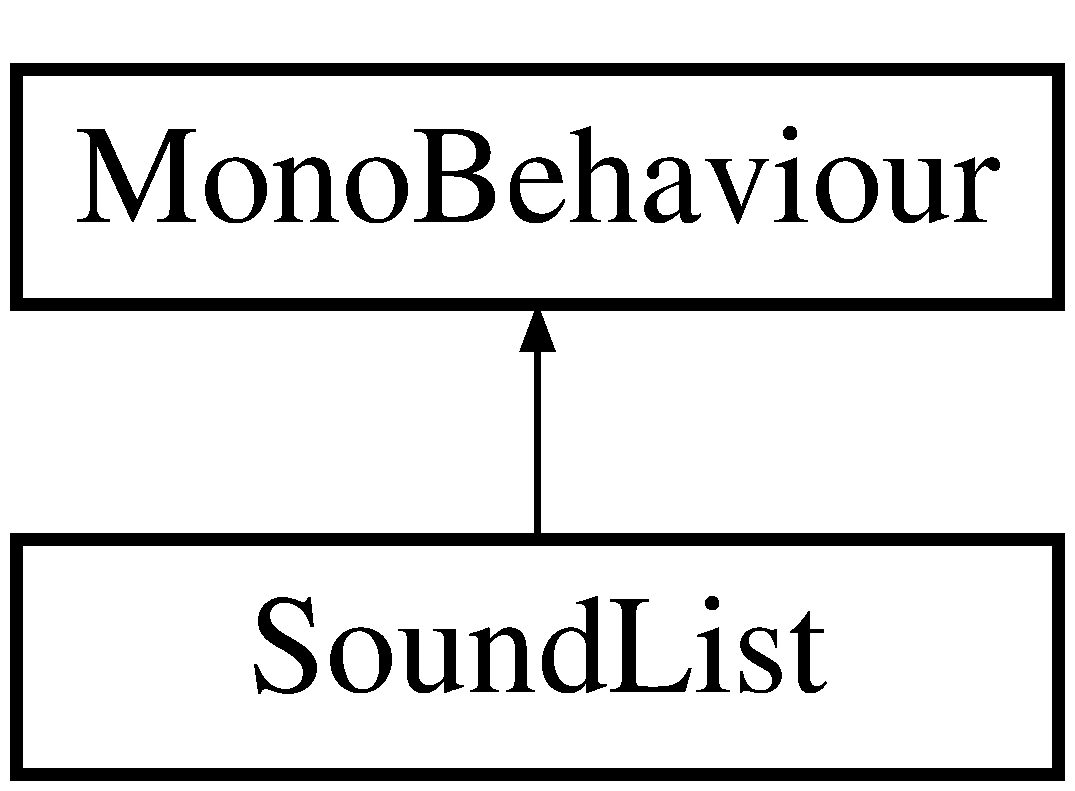
\includegraphics[height=2.000000cm]{class_sound_list}
\end{center}
\end{figure}
\subsection*{Properties}
\begin{DoxyCompactItemize}
\item 
\hyperlink{class_sound_table}{Sound\+Table} {\bfseries Table}\hspace{0.3cm}{\ttfamily  \mbox{[}get\mbox{]}}\hypertarget{class_sound_list_a3561841d0e853f881b3d3b91576551e3}{}\label{class_sound_list_a3561841d0e853f881b3d3b91576551e3}

\end{DoxyCompactItemize}


\subsection{Detailed Description}
再生する音のリスト 



The documentation for this class was generated from the following file\+:\begin{DoxyCompactItemize}
\item 
Scripts/\+Sound/Sound\+List.\+cs\end{DoxyCompactItemize}

\hypertarget{class_sound_manager}{}\section{Sound\+Manager Class Reference}
\label{class_sound_manager}\index{Sound\+Manager@{Sound\+Manager}}


サウンドマネージャー  


Inheritance diagram for Sound\+Manager\+:\begin{figure}[H]
\begin{center}
\leavevmode
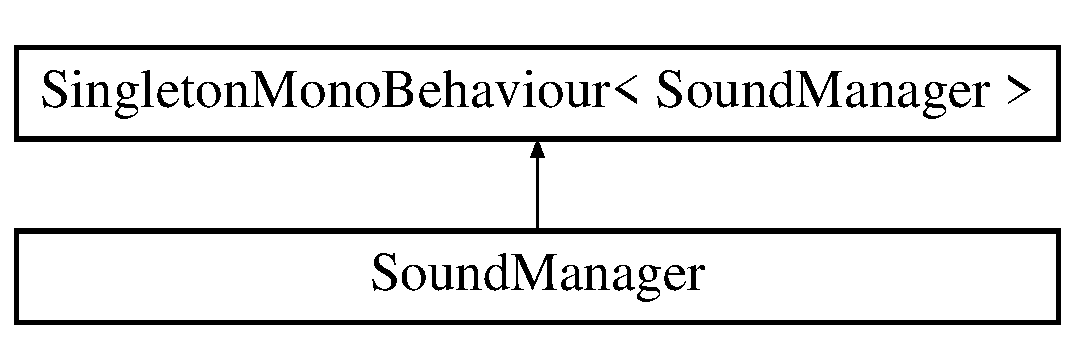
\includegraphics[height=2.000000cm]{class_sound_manager}
\end{center}
\end{figure}
\subsection*{Public Member Functions}
\begin{DoxyCompactItemize}
\item 
delegate void {\bfseries Fade\+In\+Finished\+Func} ()\hypertarget{class_sound_manager_afd4c36c3c486f23f9ee6bf399444659d}{}\label{class_sound_manager_afd4c36c3c486f23f9ee6bf399444659d}

\item 
delegate void {\bfseries Fade\+Out\+Finished\+Func} ()\hypertarget{class_sound_manager_a56961e7c98925bbbed7666ce3c4ef3ab}{}\label{class_sound_manager_a56961e7c98925bbbed7666ce3c4ef3ab}

\item 
void \hyperlink{class_sound_manager_a36ec32643d2276d727460a3ab3de18df}{Clear\+Sounds\+List} ()
\begin{DoxyCompactList}\small\item\em リストのクリア \end{DoxyCompactList}\item 
void \hyperlink{class_sound_manager_a860981b17851570fd3a6d856987e48a1}{Set\+Sounds\+List} (\hyperlink{class_sound_table}{Sound\+Table} list)
\begin{DoxyCompactList}\small\item\em リストのセット \end{DoxyCompactList}\item 
void \hyperlink{class_sound_manager_ae923cec5a1bb1887a003cc2cf46ac08c}{Set\+Sound\+List} (\hyperlink{class_sound_list}{Sound\+List} list)
\begin{DoxyCompactList}\small\item\em リストのセット \end{DoxyCompactList}\item 
void \hyperlink{class_sound_manager_a8304f6c972f1b647f169f72544229f39}{Play} (string key, int channel\+Index=0, bool is\+Loop=false)
\begin{DoxyCompactList}\small\item\em 再生 \end{DoxyCompactList}\item 
void \hyperlink{class_sound_manager_a1c7c9d6ec13a3e973d6b7d35967d3e88}{Play} (int sound\+Index, int channel\+Index=0, bool is\+Loop=false)
\begin{DoxyCompactList}\small\item\em 再生 \end{DoxyCompactList}\item 
void \hyperlink{class_sound_manager_ae07fcf059f70d28547743aa58be78381}{Play\+On\+B\+GM} (string key, int channel\+Index=0)
\begin{DoxyCompactList}\small\item\em B\+G\+M用の再生(ループ) \end{DoxyCompactList}\item 
void \hyperlink{class_sound_manager_a5f049a14d661802e4ccd32bbf44c03c2}{Play\+On\+B\+GM} (int sound\+Index, int channel\+Index=0)
\begin{DoxyCompactList}\small\item\em B\+G\+M用の再生(ループ) \end{DoxyCompactList}\item 
void \hyperlink{class_sound_manager_a77140d592dfb496cf7def31f7880f9ea}{Play\+On\+SE} (string key, float volume=1.\+0f)
\begin{DoxyCompactList}\small\item\em S\+E用の再生(一度) \end{DoxyCompactList}\item 
void \hyperlink{class_sound_manager_a730961318ec947dfbd2a0a4dd8cb9642}{Play\+On\+SE} (string key, int channel\+Index, float volume=1.\+0f)
\begin{DoxyCompactList}\small\item\em S\+E用の再生(一度) \end{DoxyCompactList}\item 
void \hyperlink{class_sound_manager_ae61ef29d24c0df5478fced7a2c2b8998}{Play\+On\+SE} (int sound\+Index, float volume=1.\+0f)
\begin{DoxyCompactList}\small\item\em S\+E用の再生(一度) \end{DoxyCompactList}\item 
void \hyperlink{class_sound_manager_ab91718ea6321db485010e776438bc8d6}{Play\+On\+SE} (int sound\+Index, int channel\+Index, float volume=1.\+0f)
\begin{DoxyCompactList}\small\item\em S\+E用の再生(一度) \end{DoxyCompactList}\item 
void \hyperlink{class_sound_manager_a9dba56ed360cd252930b9f20539244cd}{Pause} (int channel\+Index)
\begin{DoxyCompactList}\small\item\em 一時停止 \end{DoxyCompactList}\item 
void \hyperlink{class_sound_manager_ab25efe5f76915409d0cccef8dfa93464}{Un\+Pause} (int channel\+Index)
\begin{DoxyCompactList}\small\item\em 一時停止の解除 \end{DoxyCompactList}\item 
void \hyperlink{class_sound_manager_a4b049d53b4fd9137a900d0b44c555a60}{Stop} (int channel\+Index)
\begin{DoxyCompactList}\small\item\em 停止 \end{DoxyCompactList}\item 
Audio\+Source \hyperlink{class_sound_manager_ae9f3da934103d1d6fa7901f3e60d5ccb}{Get\+Channel} (int channel\+Index)
\begin{DoxyCompactList}\small\item\em 登録したチャネル(\+Audio\+Source)の取得 \end{DoxyCompactList}\item 
I\+Enumerator \hyperlink{class_sound_manager_aeb06497852c55c68d829e9cd2b6c8c0c}{Fade\+In\+Coroutine} (float frame, float volume=0.\+0f, int channel\+Index=0, Fade\+In\+Finished\+Func func=null)
\begin{DoxyCompactList}\small\item\em フェードインするコルーチン(小さくなる方) \end{DoxyCompactList}\item 
I\+Enumerator \hyperlink{class_sound_manager_a835a7e59622535078cdb6e705d74a340}{Fade\+Out\+Coroutine} (float frame, float volume=1.\+0f, int channel\+Index=0, Fade\+Out\+Finished\+Func func=null)
\begin{DoxyCompactList}\small\item\em フェードアウトするコルーチン(大きくなる方) \end{DoxyCompactList}\item 
void \hyperlink{class_sound_manager_aed0690aa358d5d5c14febad7f7a14054}{Start\+Sound\+Fade\+In} (float frame, float volume=0.\+0f, int channel\+Index=0, Fade\+In\+Finished\+Func func=null)
\begin{DoxyCompactList}\small\item\em フェードイン(小さくなる)の開始命令 \end{DoxyCompactList}\item 
void \hyperlink{class_sound_manager_a008ec30f5bbbddb9268ad1bb0fc4b1b2}{Start\+Sound\+Fade\+Out} (float frame, float volume=1.\+0f, int channel\+Index=0, Fade\+Out\+Finished\+Func func=null)
\begin{DoxyCompactList}\small\item\em フェードアウト(大きくなる)の開始命令 \end{DoxyCompactList}\item 
I\+Enumerator \hyperlink{class_sound_manager_ae0b3882cf2d76b12e8ddbaf66d338ba6}{Sound\+Fade\+In\+All\+Coroutine} (float frame, float volume=0.\+0f, Fade\+In\+Finished\+Func func=null)
\begin{DoxyCompactList}\small\item\em 全チャネルをフェードインさせるコルーチン(小さくする) \end{DoxyCompactList}\item 
I\+Enumerator \hyperlink{class_sound_manager_af73150a7037521925d280cf2bc991c84}{Sound\+Fade\+Out\+All\+Coroutine} (float frame, float volume=1.\+0f, Fade\+Out\+Finished\+Func func=null)
\begin{DoxyCompactList}\small\item\em 全チャネルをフェードアウトさせるコルーチン(大きくする) \end{DoxyCompactList}\item 
void \hyperlink{class_sound_manager_a4008b5901ae32bf230593c35a322a9d1}{Start\+Sound\+Fade\+In\+All} (float frame, float volume=0.\+0f, Fade\+In\+Finished\+Func func=null)
\begin{DoxyCompactList}\small\item\em 全チャネルのフェードイン開始命令 \end{DoxyCompactList}\item 
void \hyperlink{class_sound_manager_a9645299a9bb7cf0056abe29e8a14e32e}{Start\+Sound\+Fade\+Out\+All} (float frame, float volume=1.\+0f, Fade\+Out\+Finished\+Func func=null)
\begin{DoxyCompactList}\small\item\em 全チャネルのフェードアウト開始命令 \end{DoxyCompactList}\end{DoxyCompactItemize}
\subsection*{Properties}
\begin{DoxyCompactItemize}
\item 
bool {\bfseries is\+Fade}\hspace{0.3cm}{\ttfamily  \mbox{[}get\mbox{]}}\hypertarget{class_sound_manager_ad1424367cc1cbdf1c015fa0923a18c27}{}\label{class_sound_manager_ad1424367cc1cbdf1c015fa0923a18c27}

\end{DoxyCompactItemize}


\subsection{Detailed Description}
サウンドマネージャー 



\subsection{Member Function Documentation}
\index{Sound\+Manager@{Sound\+Manager}!Clear\+Sounds\+List@{Clear\+Sounds\+List}}
\index{Clear\+Sounds\+List@{Clear\+Sounds\+List}!Sound\+Manager@{Sound\+Manager}}
\subsubsection[{\texorpdfstring{Clear\+Sounds\+List()}{ClearSoundsList()}}]{\setlength{\rightskip}{0pt plus 5cm}void Sound\+Manager.\+Clear\+Sounds\+List (
\begin{DoxyParamCaption}
{}
\end{DoxyParamCaption}
)\hspace{0.3cm}{\ttfamily [inline]}}\hypertarget{class_sound_manager_a36ec32643d2276d727460a3ab3de18df}{}\label{class_sound_manager_a36ec32643d2276d727460a3ab3de18df}


リストのクリア 

\index{Sound\+Manager@{Sound\+Manager}!Fade\+In\+Coroutine@{Fade\+In\+Coroutine}}
\index{Fade\+In\+Coroutine@{Fade\+In\+Coroutine}!Sound\+Manager@{Sound\+Manager}}
\subsubsection[{\texorpdfstring{Fade\+In\+Coroutine(float frame, float volume=0.\+0f, int channel\+Index=0, Fade\+In\+Finished\+Func func=null)}{FadeInCoroutine(float frame, float volume=0.0f, int channelIndex=0, FadeInFinishedFunc func=null)}}]{\setlength{\rightskip}{0pt plus 5cm}I\+Enumerator Sound\+Manager.\+Fade\+In\+Coroutine (
\begin{DoxyParamCaption}
\item[{float}]{frame, }
\item[{float}]{volume = {\ttfamily 0.0f}, }
\item[{int}]{channel\+Index = {\ttfamily 0}, }
\item[{Fade\+In\+Finished\+Func}]{func = {\ttfamily null}}
\end{DoxyParamCaption}
)\hspace{0.3cm}{\ttfamily [inline]}}\hypertarget{class_sound_manager_aeb06497852c55c68d829e9cd2b6c8c0c}{}\label{class_sound_manager_aeb06497852c55c68d829e9cd2b6c8c0c}


フェードインするコルーチン(小さくなる方) 


\begin{DoxyParams}{Parameters}
{\em frame} & フェードさせるフレーム\\
\hline
{\em volume} & フェード先のボリューム(0.\+0~1.0)\\
\hline
{\em fade\+In\+Finished} & フェードイン終了後に行う関数\\
\hline
\end{DoxyParams}
\begin{DoxyReturn}{Returns}

\end{DoxyReturn}
\index{Sound\+Manager@{Sound\+Manager}!Fade\+Out\+Coroutine@{Fade\+Out\+Coroutine}}
\index{Fade\+Out\+Coroutine@{Fade\+Out\+Coroutine}!Sound\+Manager@{Sound\+Manager}}
\subsubsection[{\texorpdfstring{Fade\+Out\+Coroutine(float frame, float volume=1.\+0f, int channel\+Index=0, Fade\+Out\+Finished\+Func func=null)}{FadeOutCoroutine(float frame, float volume=1.0f, int channelIndex=0, FadeOutFinishedFunc func=null)}}]{\setlength{\rightskip}{0pt plus 5cm}I\+Enumerator Sound\+Manager.\+Fade\+Out\+Coroutine (
\begin{DoxyParamCaption}
\item[{float}]{frame, }
\item[{float}]{volume = {\ttfamily 1.0f}, }
\item[{int}]{channel\+Index = {\ttfamily 0}, }
\item[{Fade\+Out\+Finished\+Func}]{func = {\ttfamily null}}
\end{DoxyParamCaption}
)\hspace{0.3cm}{\ttfamily [inline]}}\hypertarget{class_sound_manager_a835a7e59622535078cdb6e705d74a340}{}\label{class_sound_manager_a835a7e59622535078cdb6e705d74a340}


フェードアウトするコルーチン(大きくなる方) 


\begin{DoxyParams}{Parameters}
{\em frame} & フェードさせるフレーム\\
\hline
{\em volume} & フェード先のボリューム(0.\+0~1.0)\\
\hline
{\em fade\+In\+Finished} & フェードアウト終了後に行う関数\\
\hline
\end{DoxyParams}
\begin{DoxyReturn}{Returns}

\end{DoxyReturn}
\index{Sound\+Manager@{Sound\+Manager}!Get\+Channel@{Get\+Channel}}
\index{Get\+Channel@{Get\+Channel}!Sound\+Manager@{Sound\+Manager}}
\subsubsection[{\texorpdfstring{Get\+Channel(int channel\+Index)}{GetChannel(int channelIndex)}}]{\setlength{\rightskip}{0pt plus 5cm}Audio\+Source Sound\+Manager.\+Get\+Channel (
\begin{DoxyParamCaption}
\item[{int}]{channel\+Index}
\end{DoxyParamCaption}
)\hspace{0.3cm}{\ttfamily [inline]}}\hypertarget{class_sound_manager_ae9f3da934103d1d6fa7901f3e60d5ccb}{}\label{class_sound_manager_ae9f3da934103d1d6fa7901f3e60d5ccb}


登録したチャネル(\+Audio\+Source)の取得 


\begin{DoxyParams}{Parameters}
{\em channel\+Index} & チャネルの番号\\
\hline
\end{DoxyParams}
\begin{DoxyReturn}{Returns}

\end{DoxyReturn}
\index{Sound\+Manager@{Sound\+Manager}!Pause@{Pause}}
\index{Pause@{Pause}!Sound\+Manager@{Sound\+Manager}}
\subsubsection[{\texorpdfstring{Pause(int channel\+Index)}{Pause(int channelIndex)}}]{\setlength{\rightskip}{0pt plus 5cm}void Sound\+Manager.\+Pause (
\begin{DoxyParamCaption}
\item[{int}]{channel\+Index}
\end{DoxyParamCaption}
)\hspace{0.3cm}{\ttfamily [inline]}}\hypertarget{class_sound_manager_a9dba56ed360cd252930b9f20539244cd}{}\label{class_sound_manager_a9dba56ed360cd252930b9f20539244cd}


一時停止 


\begin{DoxyParams}{Parameters}
{\em channel\+Index} & 一時停止するチャネルの番号\\
\hline
\end{DoxyParams}
\index{Sound\+Manager@{Sound\+Manager}!Play@{Play}}
\index{Play@{Play}!Sound\+Manager@{Sound\+Manager}}
\subsubsection[{\texorpdfstring{Play(string key, int channel\+Index=0, bool is\+Loop=false)}{Play(string key, int channelIndex=0, bool isLoop=false)}}]{\setlength{\rightskip}{0pt plus 5cm}void Sound\+Manager.\+Play (
\begin{DoxyParamCaption}
\item[{string}]{key, }
\item[{int}]{channel\+Index = {\ttfamily 0}, }
\item[{bool}]{is\+Loop = {\ttfamily false}}
\end{DoxyParamCaption}
)\hspace{0.3cm}{\ttfamily [inline]}}\hypertarget{class_sound_manager_a8304f6c972f1b647f169f72544229f39}{}\label{class_sound_manager_a8304f6c972f1b647f169f72544229f39}


再生 


\begin{DoxyParams}{Parameters}
{\em key} & 登録されたサウンドリストのハッシュキー\\
\hline
{\em channel\+Index} & 鳴らすチャネルの番号\\
\hline
{\em is\+Loop} & ループ有無\\
\hline
\end{DoxyParams}
\index{Sound\+Manager@{Sound\+Manager}!Play@{Play}}
\index{Play@{Play}!Sound\+Manager@{Sound\+Manager}}
\subsubsection[{\texorpdfstring{Play(int sound\+Index, int channel\+Index=0, bool is\+Loop=false)}{Play(int soundIndex, int channelIndex=0, bool isLoop=false)}}]{\setlength{\rightskip}{0pt plus 5cm}void Sound\+Manager.\+Play (
\begin{DoxyParamCaption}
\item[{int}]{sound\+Index, }
\item[{int}]{channel\+Index = {\ttfamily 0}, }
\item[{bool}]{is\+Loop = {\ttfamily false}}
\end{DoxyParamCaption}
)\hspace{0.3cm}{\ttfamily [inline]}}\hypertarget{class_sound_manager_a1c7c9d6ec13a3e973d6b7d35967d3e88}{}\label{class_sound_manager_a1c7c9d6ec13a3e973d6b7d35967d3e88}


再生 


\begin{DoxyParams}{Parameters}
{\em sound\+Index} & 登録されたサウンドリストのインデックス\\
\hline
{\em channel\+Index} & 鳴らすチャネルの番号\\
\hline
{\em is\+Loop} & ループ有無\\
\hline
\end{DoxyParams}
\index{Sound\+Manager@{Sound\+Manager}!Play\+On\+B\+GM@{Play\+On\+B\+GM}}
\index{Play\+On\+B\+GM@{Play\+On\+B\+GM}!Sound\+Manager@{Sound\+Manager}}
\subsubsection[{\texorpdfstring{Play\+On\+B\+G\+M(string key, int channel\+Index=0)}{PlayOnBGM(string key, int channelIndex=0)}}]{\setlength{\rightskip}{0pt plus 5cm}void Sound\+Manager.\+Play\+On\+B\+GM (
\begin{DoxyParamCaption}
\item[{string}]{key, }
\item[{int}]{channel\+Index = {\ttfamily 0}}
\end{DoxyParamCaption}
)\hspace{0.3cm}{\ttfamily [inline]}}\hypertarget{class_sound_manager_ae07fcf059f70d28547743aa58be78381}{}\label{class_sound_manager_ae07fcf059f70d28547743aa58be78381}


B\+G\+M用の再生(ループ) 


\begin{DoxyParams}{Parameters}
{\em key} & 登録されたサウンドリストのハッシュキー\\
\hline
{\em channel\+Index} & 鳴らすチャネルの番号\\
\hline
\end{DoxyParams}
\index{Sound\+Manager@{Sound\+Manager}!Play\+On\+B\+GM@{Play\+On\+B\+GM}}
\index{Play\+On\+B\+GM@{Play\+On\+B\+GM}!Sound\+Manager@{Sound\+Manager}}
\subsubsection[{\texorpdfstring{Play\+On\+B\+G\+M(int sound\+Index, int channel\+Index=0)}{PlayOnBGM(int soundIndex, int channelIndex=0)}}]{\setlength{\rightskip}{0pt plus 5cm}void Sound\+Manager.\+Play\+On\+B\+GM (
\begin{DoxyParamCaption}
\item[{int}]{sound\+Index, }
\item[{int}]{channel\+Index = {\ttfamily 0}}
\end{DoxyParamCaption}
)\hspace{0.3cm}{\ttfamily [inline]}}\hypertarget{class_sound_manager_a5f049a14d661802e4ccd32bbf44c03c2}{}\label{class_sound_manager_a5f049a14d661802e4ccd32bbf44c03c2}


B\+G\+M用の再生(ループ) 


\begin{DoxyParams}{Parameters}
{\em sound\+Index} & 登録されたサウンドリストのインデックス\\
\hline
{\em channel\+Index} & 鳴らすチャネルの番号\\
\hline
\end{DoxyParams}
\index{Sound\+Manager@{Sound\+Manager}!Play\+On\+SE@{Play\+On\+SE}}
\index{Play\+On\+SE@{Play\+On\+SE}!Sound\+Manager@{Sound\+Manager}}
\subsubsection[{\texorpdfstring{Play\+On\+S\+E(string key, float volume=1.\+0f)}{PlayOnSE(string key, float volume=1.0f)}}]{\setlength{\rightskip}{0pt plus 5cm}void Sound\+Manager.\+Play\+On\+SE (
\begin{DoxyParamCaption}
\item[{string}]{key, }
\item[{float}]{volume = {\ttfamily 1.0f}}
\end{DoxyParamCaption}
)\hspace{0.3cm}{\ttfamily [inline]}}\hypertarget{class_sound_manager_a77140d592dfb496cf7def31f7880f9ea}{}\label{class_sound_manager_a77140d592dfb496cf7def31f7880f9ea}


S\+E用の再生(一度) 


\begin{DoxyParams}{Parameters}
{\em key} & 登録されたサウンドリストのハッシュキー\\
\hline
{\em volume} & 音量(0.\+0~1.0)\\
\hline
\end{DoxyParams}
\index{Sound\+Manager@{Sound\+Manager}!Play\+On\+SE@{Play\+On\+SE}}
\index{Play\+On\+SE@{Play\+On\+SE}!Sound\+Manager@{Sound\+Manager}}
\subsubsection[{\texorpdfstring{Play\+On\+S\+E(string key, int channel\+Index, float volume=1.\+0f)}{PlayOnSE(string key, int channelIndex, float volume=1.0f)}}]{\setlength{\rightskip}{0pt plus 5cm}void Sound\+Manager.\+Play\+On\+SE (
\begin{DoxyParamCaption}
\item[{string}]{key, }
\item[{int}]{channel\+Index, }
\item[{float}]{volume = {\ttfamily 1.0f}}
\end{DoxyParamCaption}
)\hspace{0.3cm}{\ttfamily [inline]}}\hypertarget{class_sound_manager_a730961318ec947dfbd2a0a4dd8cb9642}{}\label{class_sound_manager_a730961318ec947dfbd2a0a4dd8cb9642}


S\+E用の再生(一度) 


\begin{DoxyParams}{Parameters}
{\em key} & 登録されたサウンドリストのハッシュキー\\
\hline
{\em volume} & 音量(0.\+0~1.0)\\
\hline
\end{DoxyParams}
\index{Sound\+Manager@{Sound\+Manager}!Play\+On\+SE@{Play\+On\+SE}}
\index{Play\+On\+SE@{Play\+On\+SE}!Sound\+Manager@{Sound\+Manager}}
\subsubsection[{\texorpdfstring{Play\+On\+S\+E(int sound\+Index, float volume=1.\+0f)}{PlayOnSE(int soundIndex, float volume=1.0f)}}]{\setlength{\rightskip}{0pt plus 5cm}void Sound\+Manager.\+Play\+On\+SE (
\begin{DoxyParamCaption}
\item[{int}]{sound\+Index, }
\item[{float}]{volume = {\ttfamily 1.0f}}
\end{DoxyParamCaption}
)\hspace{0.3cm}{\ttfamily [inline]}}\hypertarget{class_sound_manager_ae61ef29d24c0df5478fced7a2c2b8998}{}\label{class_sound_manager_ae61ef29d24c0df5478fced7a2c2b8998}


S\+E用の再生(一度) 


\begin{DoxyParams}{Parameters}
{\em sound\+Index} & 登録されたサウンドリストのインデックス\\
\hline
{\em volume} & 音量(0.\+0~1.0)\\
\hline
\end{DoxyParams}
\index{Sound\+Manager@{Sound\+Manager}!Play\+On\+SE@{Play\+On\+SE}}
\index{Play\+On\+SE@{Play\+On\+SE}!Sound\+Manager@{Sound\+Manager}}
\subsubsection[{\texorpdfstring{Play\+On\+S\+E(int sound\+Index, int channel\+Index, float volume=1.\+0f)}{PlayOnSE(int soundIndex, int channelIndex, float volume=1.0f)}}]{\setlength{\rightskip}{0pt plus 5cm}void Sound\+Manager.\+Play\+On\+SE (
\begin{DoxyParamCaption}
\item[{int}]{sound\+Index, }
\item[{int}]{channel\+Index, }
\item[{float}]{volume = {\ttfamily 1.0f}}
\end{DoxyParamCaption}
)\hspace{0.3cm}{\ttfamily [inline]}}\hypertarget{class_sound_manager_ab91718ea6321db485010e776438bc8d6}{}\label{class_sound_manager_ab91718ea6321db485010e776438bc8d6}


S\+E用の再生(一度) 


\begin{DoxyParams}{Parameters}
{\em sound\+Index} & 登録されたサウンドリストのインデックス\\
\hline
{\em volume} & 音量(0.\+0~1.0)\\
\hline
\end{DoxyParams}
\index{Sound\+Manager@{Sound\+Manager}!Set\+Sound\+List@{Set\+Sound\+List}}
\index{Set\+Sound\+List@{Set\+Sound\+List}!Sound\+Manager@{Sound\+Manager}}
\subsubsection[{\texorpdfstring{Set\+Sound\+List(\+Sound\+List list)}{SetSoundList(SoundList list)}}]{\setlength{\rightskip}{0pt plus 5cm}void Sound\+Manager.\+Set\+Sound\+List (
\begin{DoxyParamCaption}
\item[{{\bf Sound\+List}}]{list}
\end{DoxyParamCaption}
)\hspace{0.3cm}{\ttfamily [inline]}}\hypertarget{class_sound_manager_ae923cec5a1bb1887a003cc2cf46ac08c}{}\label{class_sound_manager_ae923cec5a1bb1887a003cc2cf46ac08c}


リストのセット 


\begin{DoxyParams}{Parameters}
{\em list} & \\
\hline
\end{DoxyParams}
\index{Sound\+Manager@{Sound\+Manager}!Set\+Sounds\+List@{Set\+Sounds\+List}}
\index{Set\+Sounds\+List@{Set\+Sounds\+List}!Sound\+Manager@{Sound\+Manager}}
\subsubsection[{\texorpdfstring{Set\+Sounds\+List(\+Sound\+Table list)}{SetSoundsList(SoundTable list)}}]{\setlength{\rightskip}{0pt plus 5cm}void Sound\+Manager.\+Set\+Sounds\+List (
\begin{DoxyParamCaption}
\item[{{\bf Sound\+Table}}]{list}
\end{DoxyParamCaption}
)\hspace{0.3cm}{\ttfamily [inline]}}\hypertarget{class_sound_manager_a860981b17851570fd3a6d856987e48a1}{}\label{class_sound_manager_a860981b17851570fd3a6d856987e48a1}


リストのセット 


\begin{DoxyParams}{Parameters}
{\em list} & \\
\hline
\end{DoxyParams}
\index{Sound\+Manager@{Sound\+Manager}!Sound\+Fade\+In\+All\+Coroutine@{Sound\+Fade\+In\+All\+Coroutine}}
\index{Sound\+Fade\+In\+All\+Coroutine@{Sound\+Fade\+In\+All\+Coroutine}!Sound\+Manager@{Sound\+Manager}}
\subsubsection[{\texorpdfstring{Sound\+Fade\+In\+All\+Coroutine(float frame, float volume=0.\+0f, Fade\+In\+Finished\+Func func=null)}{SoundFadeInAllCoroutine(float frame, float volume=0.0f, FadeInFinishedFunc func=null)}}]{\setlength{\rightskip}{0pt plus 5cm}I\+Enumerator Sound\+Manager.\+Sound\+Fade\+In\+All\+Coroutine (
\begin{DoxyParamCaption}
\item[{float}]{frame, }
\item[{float}]{volume = {\ttfamily 0.0f}, }
\item[{Fade\+In\+Finished\+Func}]{func = {\ttfamily null}}
\end{DoxyParamCaption}
)\hspace{0.3cm}{\ttfamily [inline]}}\hypertarget{class_sound_manager_ae0b3882cf2d76b12e8ddbaf66d338ba6}{}\label{class_sound_manager_ae0b3882cf2d76b12e8ddbaf66d338ba6}


全チャネルをフェードインさせるコルーチン(小さくする) 


\begin{DoxyParams}{Parameters}
{\em frame} & フェードさせるフレーム\\
\hline
{\em volume} & フェード先のボリューム(0.\+0~1.0)\\
\hline
{\em func} & フェードイン終了後に行う関数\\
\hline
\end{DoxyParams}
\begin{DoxyReturn}{Returns}

\end{DoxyReturn}
\index{Sound\+Manager@{Sound\+Manager}!Sound\+Fade\+Out\+All\+Coroutine@{Sound\+Fade\+Out\+All\+Coroutine}}
\index{Sound\+Fade\+Out\+All\+Coroutine@{Sound\+Fade\+Out\+All\+Coroutine}!Sound\+Manager@{Sound\+Manager}}
\subsubsection[{\texorpdfstring{Sound\+Fade\+Out\+All\+Coroutine(float frame, float volume=1.\+0f, Fade\+Out\+Finished\+Func func=null)}{SoundFadeOutAllCoroutine(float frame, float volume=1.0f, FadeOutFinishedFunc func=null)}}]{\setlength{\rightskip}{0pt plus 5cm}I\+Enumerator Sound\+Manager.\+Sound\+Fade\+Out\+All\+Coroutine (
\begin{DoxyParamCaption}
\item[{float}]{frame, }
\item[{float}]{volume = {\ttfamily 1.0f}, }
\item[{Fade\+Out\+Finished\+Func}]{func = {\ttfamily null}}
\end{DoxyParamCaption}
)\hspace{0.3cm}{\ttfamily [inline]}}\hypertarget{class_sound_manager_af73150a7037521925d280cf2bc991c84}{}\label{class_sound_manager_af73150a7037521925d280cf2bc991c84}


全チャネルをフェードアウトさせるコルーチン(大きくする) 


\begin{DoxyParams}{Parameters}
{\em frame} & フェードさせるフレーム\\
\hline
{\em volume} & フェード先のボリューム(0.\+0~1.0)\\
\hline
{\em func} & フェードアウト終了後に行う関数\\
\hline
\end{DoxyParams}
\begin{DoxyReturn}{Returns}

\end{DoxyReturn}
\index{Sound\+Manager@{Sound\+Manager}!Start\+Sound\+Fade\+In@{Start\+Sound\+Fade\+In}}
\index{Start\+Sound\+Fade\+In@{Start\+Sound\+Fade\+In}!Sound\+Manager@{Sound\+Manager}}
\subsubsection[{\texorpdfstring{Start\+Sound\+Fade\+In(float frame, float volume=0.\+0f, int channel\+Index=0, Fade\+In\+Finished\+Func func=null)}{StartSoundFadeIn(float frame, float volume=0.0f, int channelIndex=0, FadeInFinishedFunc func=null)}}]{\setlength{\rightskip}{0pt plus 5cm}void Sound\+Manager.\+Start\+Sound\+Fade\+In (
\begin{DoxyParamCaption}
\item[{float}]{frame, }
\item[{float}]{volume = {\ttfamily 0.0f}, }
\item[{int}]{channel\+Index = {\ttfamily 0}, }
\item[{Fade\+In\+Finished\+Func}]{func = {\ttfamily null}}
\end{DoxyParamCaption}
)\hspace{0.3cm}{\ttfamily [inline]}}\hypertarget{class_sound_manager_aed0690aa358d5d5c14febad7f7a14054}{}\label{class_sound_manager_aed0690aa358d5d5c14febad7f7a14054}


フェードイン(小さくなる)の開始命令 


\begin{DoxyParams}{Parameters}
{\em frame} & フェードさせるフレーム\\
\hline
{\em volume} & フェード先のボリューム(0.\+0~1.0)\\
\hline
{\em channel\+Index} & フェードさせるチャネルの番号\\
\hline
{\em func} & フェードイン終了後に行う関数\\
\hline
\end{DoxyParams}
\index{Sound\+Manager@{Sound\+Manager}!Start\+Sound\+Fade\+In\+All@{Start\+Sound\+Fade\+In\+All}}
\index{Start\+Sound\+Fade\+In\+All@{Start\+Sound\+Fade\+In\+All}!Sound\+Manager@{Sound\+Manager}}
\subsubsection[{\texorpdfstring{Start\+Sound\+Fade\+In\+All(float frame, float volume=0.\+0f, Fade\+In\+Finished\+Func func=null)}{StartSoundFadeInAll(float frame, float volume=0.0f, FadeInFinishedFunc func=null)}}]{\setlength{\rightskip}{0pt plus 5cm}void Sound\+Manager.\+Start\+Sound\+Fade\+In\+All (
\begin{DoxyParamCaption}
\item[{float}]{frame, }
\item[{float}]{volume = {\ttfamily 0.0f}, }
\item[{Fade\+In\+Finished\+Func}]{func = {\ttfamily null}}
\end{DoxyParamCaption}
)\hspace{0.3cm}{\ttfamily [inline]}}\hypertarget{class_sound_manager_a4008b5901ae32bf230593c35a322a9d1}{}\label{class_sound_manager_a4008b5901ae32bf230593c35a322a9d1}


全チャネルのフェードイン開始命令 


\begin{DoxyParams}{Parameters}
{\em frame} & フェードさせるフレーム\\
\hline
{\em volume} & フェード先のボリューム\\
\hline
{\em func} & フェードイン終了後に行う関数\\
\hline
\end{DoxyParams}
\index{Sound\+Manager@{Sound\+Manager}!Start\+Sound\+Fade\+Out@{Start\+Sound\+Fade\+Out}}
\index{Start\+Sound\+Fade\+Out@{Start\+Sound\+Fade\+Out}!Sound\+Manager@{Sound\+Manager}}
\subsubsection[{\texorpdfstring{Start\+Sound\+Fade\+Out(float frame, float volume=1.\+0f, int channel\+Index=0, Fade\+Out\+Finished\+Func func=null)}{StartSoundFadeOut(float frame, float volume=1.0f, int channelIndex=0, FadeOutFinishedFunc func=null)}}]{\setlength{\rightskip}{0pt plus 5cm}void Sound\+Manager.\+Start\+Sound\+Fade\+Out (
\begin{DoxyParamCaption}
\item[{float}]{frame, }
\item[{float}]{volume = {\ttfamily 1.0f}, }
\item[{int}]{channel\+Index = {\ttfamily 0}, }
\item[{Fade\+Out\+Finished\+Func}]{func = {\ttfamily null}}
\end{DoxyParamCaption}
)\hspace{0.3cm}{\ttfamily [inline]}}\hypertarget{class_sound_manager_a008ec30f5bbbddb9268ad1bb0fc4b1b2}{}\label{class_sound_manager_a008ec30f5bbbddb9268ad1bb0fc4b1b2}


フェードアウト(大きくなる)の開始命令 


\begin{DoxyParams}{Parameters}
{\em frame} & フェードさせるフレーム\\
\hline
{\em volume} & フェード先のボリューム(0.\+0~1.0)\\
\hline
{\em channel\+Index} & フェードさせるチャネルの番号\\
\hline
{\em func} & フェードアウト終了後に行う関数\\
\hline
\end{DoxyParams}
\index{Sound\+Manager@{Sound\+Manager}!Start\+Sound\+Fade\+Out\+All@{Start\+Sound\+Fade\+Out\+All}}
\index{Start\+Sound\+Fade\+Out\+All@{Start\+Sound\+Fade\+Out\+All}!Sound\+Manager@{Sound\+Manager}}
\subsubsection[{\texorpdfstring{Start\+Sound\+Fade\+Out\+All(float frame, float volume=1.\+0f, Fade\+Out\+Finished\+Func func=null)}{StartSoundFadeOutAll(float frame, float volume=1.0f, FadeOutFinishedFunc func=null)}}]{\setlength{\rightskip}{0pt plus 5cm}void Sound\+Manager.\+Start\+Sound\+Fade\+Out\+All (
\begin{DoxyParamCaption}
\item[{float}]{frame, }
\item[{float}]{volume = {\ttfamily 1.0f}, }
\item[{Fade\+Out\+Finished\+Func}]{func = {\ttfamily null}}
\end{DoxyParamCaption}
)\hspace{0.3cm}{\ttfamily [inline]}}\hypertarget{class_sound_manager_a9645299a9bb7cf0056abe29e8a14e32e}{}\label{class_sound_manager_a9645299a9bb7cf0056abe29e8a14e32e}


全チャネルのフェードアウト開始命令 


\begin{DoxyParams}{Parameters}
{\em frame} & フェードさせるフレーム\\
\hline
{\em volume} & フェード先のボリューム\\
\hline
{\em func} & フェードアウト終了後に行う関数\\
\hline
\end{DoxyParams}
\index{Sound\+Manager@{Sound\+Manager}!Stop@{Stop}}
\index{Stop@{Stop}!Sound\+Manager@{Sound\+Manager}}
\subsubsection[{\texorpdfstring{Stop(int channel\+Index)}{Stop(int channelIndex)}}]{\setlength{\rightskip}{0pt plus 5cm}void Sound\+Manager.\+Stop (
\begin{DoxyParamCaption}
\item[{int}]{channel\+Index}
\end{DoxyParamCaption}
)\hspace{0.3cm}{\ttfamily [inline]}}\hypertarget{class_sound_manager_a4b049d53b4fd9137a900d0b44c555a60}{}\label{class_sound_manager_a4b049d53b4fd9137a900d0b44c555a60}


停止 


\begin{DoxyParams}{Parameters}
{\em channel\+Index} & 停止するチャネルの番号\\
\hline
\end{DoxyParams}
\index{Sound\+Manager@{Sound\+Manager}!Un\+Pause@{Un\+Pause}}
\index{Un\+Pause@{Un\+Pause}!Sound\+Manager@{Sound\+Manager}}
\subsubsection[{\texorpdfstring{Un\+Pause(int channel\+Index)}{UnPause(int channelIndex)}}]{\setlength{\rightskip}{0pt plus 5cm}void Sound\+Manager.\+Un\+Pause (
\begin{DoxyParamCaption}
\item[{int}]{channel\+Index}
\end{DoxyParamCaption}
)\hspace{0.3cm}{\ttfamily [inline]}}\hypertarget{class_sound_manager_ab25efe5f76915409d0cccef8dfa93464}{}\label{class_sound_manager_ab25efe5f76915409d0cccef8dfa93464}


一時停止の解除 


\begin{DoxyParams}{Parameters}
{\em channel\+Index} & 一時停止を解除するチャネルの番号\\
\hline
\end{DoxyParams}


The documentation for this class was generated from the following file\+:\begin{DoxyCompactItemize}
\item 
Scripts/\+Sound/Sound\+Manager.\+cs\end{DoxyCompactItemize}

\hypertarget{class_sound_pair}{}\section{Sound\+Pair Class Reference}
\label{class_sound_pair}\index{Sound\+Pair@{Sound\+Pair}}
Inheritance diagram for Sound\+Pair\+:\begin{figure}[H]
\begin{center}
\leavevmode
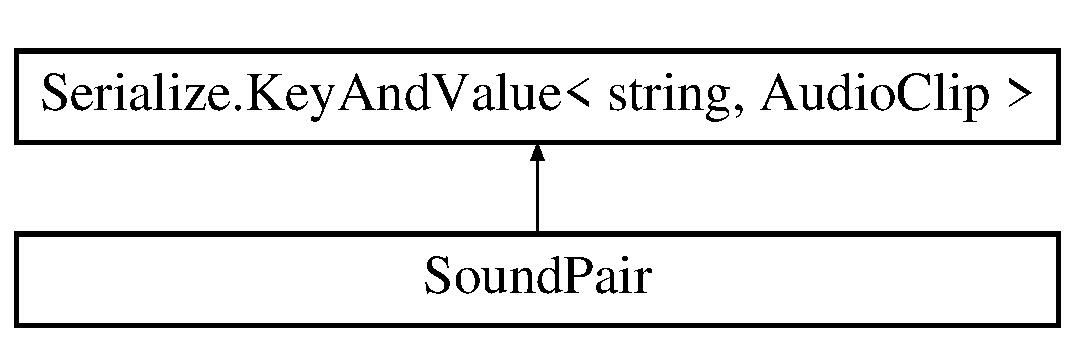
\includegraphics[height=2.000000cm]{class_sound_pair}
\end{center}
\end{figure}
\subsection*{Public Member Functions}
\begin{DoxyCompactItemize}
\item 
{\bfseries Sound\+Pair} (string key, Audio\+Clip value)\hypertarget{class_sound_pair_acfc4e92a4f017d56a6c1f05c32641c53}{}\label{class_sound_pair_acfc4e92a4f017d56a6c1f05c32641c53}

\end{DoxyCompactItemize}
\subsection*{Additional Inherited Members}


The documentation for this class was generated from the following file\+:\begin{DoxyCompactItemize}
\item 
Scripts/\+Sound/Sound\+List.\+cs\end{DoxyCompactItemize}

\hypertarget{class_sound_table}{}\section{Sound\+Table Class Reference}
\label{class_sound_table}\index{Sound\+Table@{Sound\+Table}}
Inheritance diagram for Sound\+Table\+:\begin{figure}[H]
\begin{center}
\leavevmode
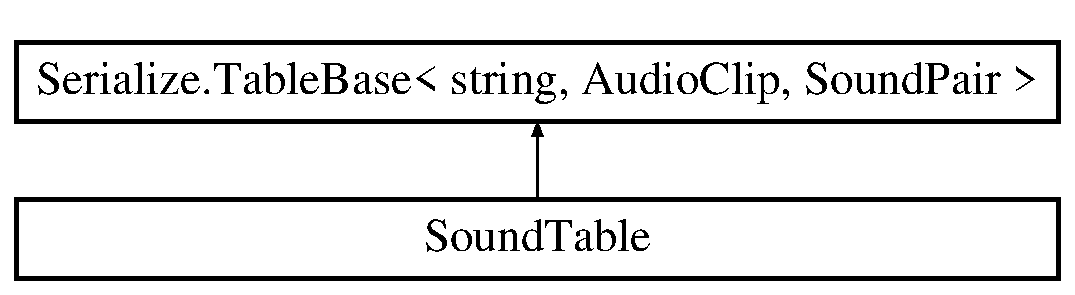
\includegraphics[height=2.000000cm]{class_sound_table}
\end{center}
\end{figure}
\subsection*{Additional Inherited Members}


The documentation for this class was generated from the following file\+:\begin{DoxyCompactItemize}
\item 
Scripts/\+Sound/Sound\+List.\+cs\end{DoxyCompactItemize}

\hypertarget{class_start_fire_works_pool}{}\section{Start\+Fire\+Works\+Pool Class Reference}
\label{class_start_fire_works_pool}\index{Start\+Fire\+Works\+Pool@{Start\+Fire\+Works\+Pool}}


スタートシーンのエフェクト用プール  


Inheritance diagram for Start\+Fire\+Works\+Pool\+:\begin{figure}[H]
\begin{center}
\leavevmode
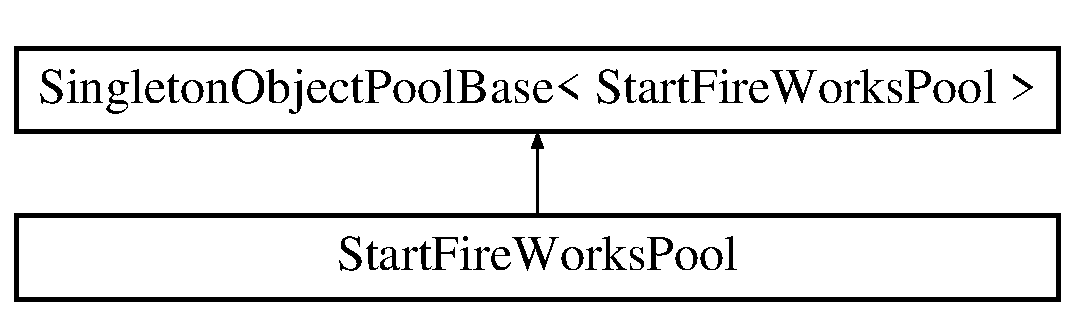
\includegraphics[height=2.000000cm]{class_start_fire_works_pool}
\end{center}
\end{figure}
\subsection*{Public Member Functions}
\begin{DoxyCompactItemize}
\item 
void {\bfseries Run} (Vector3 pos)\hypertarget{class_start_fire_works_pool_a9038d1cc7630e0508d3d8dee7179e1a4}{}\label{class_start_fire_works_pool_a9038d1cc7630e0508d3d8dee7179e1a4}

\end{DoxyCompactItemize}
\subsection*{Additional Inherited Members}


\subsection{Detailed Description}
スタートシーンのエフェクト用プール 



The documentation for this class was generated from the following file\+:\begin{DoxyCompactItemize}
\item 
Scripts/\+Object\+Pool/Start\+Fire\+Works\+Pool.\+cs\end{DoxyCompactItemize}

\hypertarget{class_start_fx_idling}{}\section{Start\+Fx\+Idling Class Reference}
\label{class_start_fx_idling}\index{Start\+Fx\+Idling@{Start\+Fx\+Idling}}


スタートシーン内の\+Fx  


Inheritance diagram for Start\+Fx\+Idling\+:\begin{figure}[H]
\begin{center}
\leavevmode
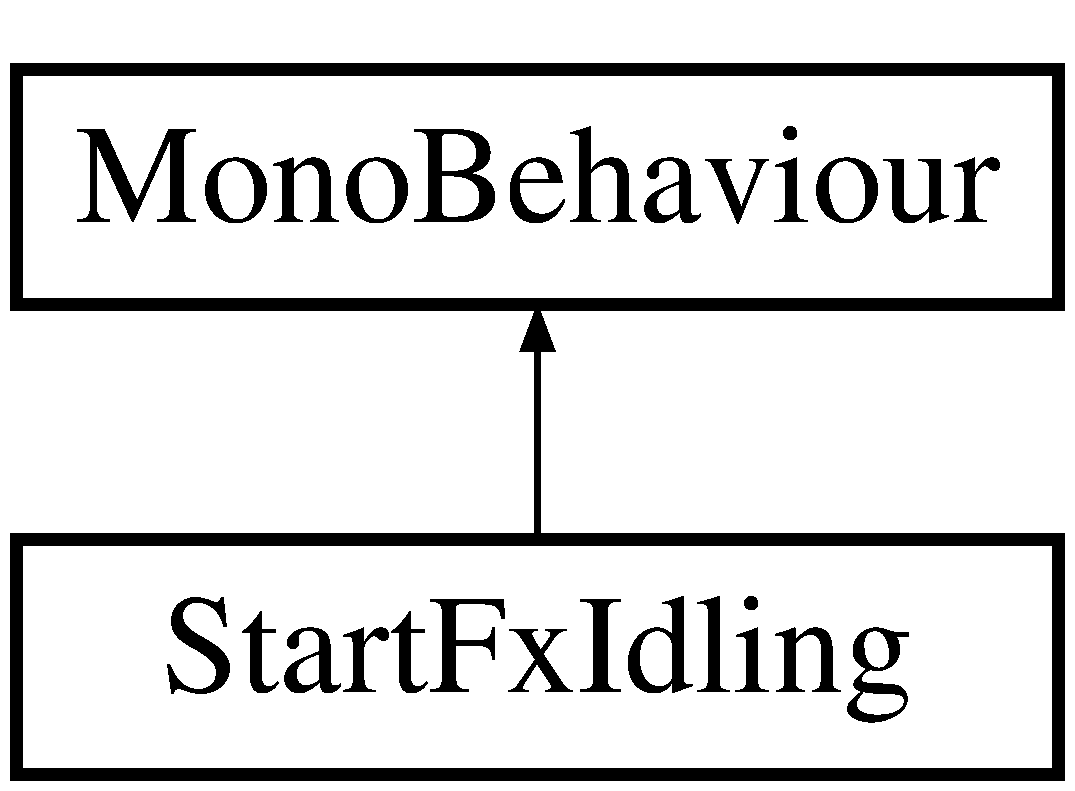
\includegraphics[height=2.000000cm]{class_start_fx_idling}
\end{center}
\end{figure}


\subsection{Detailed Description}
スタートシーン内の\+Fx 



The documentation for this class was generated from the following file\+:\begin{DoxyCompactItemize}
\item 
Scripts/\+F\+X/Start\+Fx\+Idling.\+cs\end{DoxyCompactItemize}

\hypertarget{class_start_scene_controller}{}\section{Start\+Scene\+Controller Class Reference}
\label{class_start_scene_controller}\index{Start\+Scene\+Controller@{Start\+Scene\+Controller}}


スタートシーンのコントロール  


Inheritance diagram for Start\+Scene\+Controller\+:\begin{figure}[H]
\begin{center}
\leavevmode
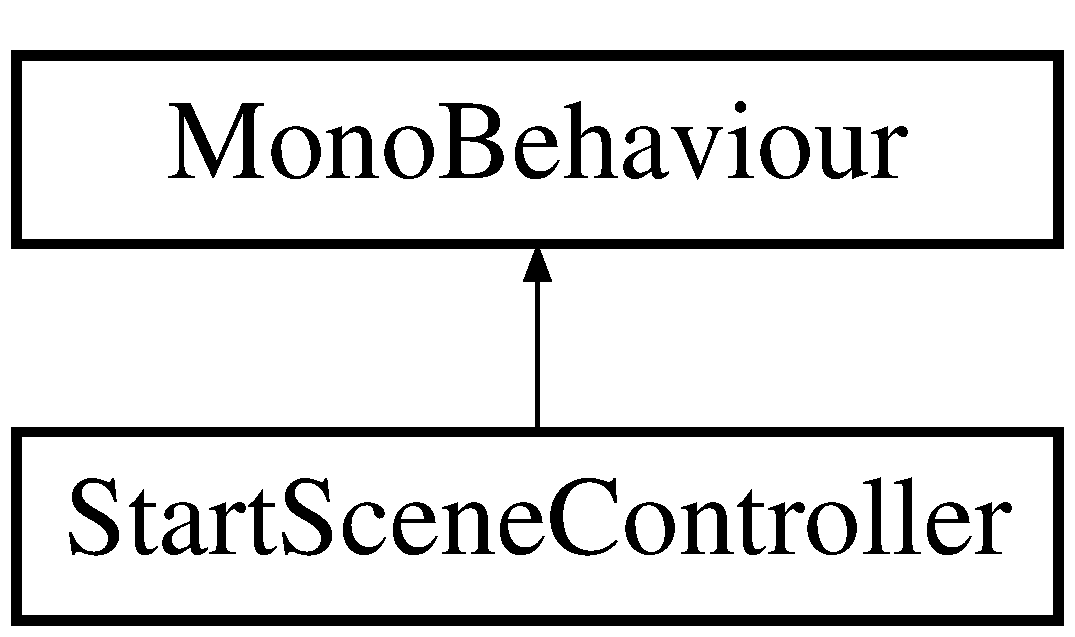
\includegraphics[height=2.000000cm]{class_start_scene_controller}
\end{center}
\end{figure}
\subsection*{Public Member Functions}
\begin{DoxyCompactItemize}
\item 
void \hyperlink{class_start_scene_controller_ac5e366920ae5020dc597d73cd37d46f6}{Game\+Start} ()
\begin{DoxyCompactList}\small\item\em ゲームスタート処理 \end{DoxyCompactList}\item 
void \hyperlink{class_start_scene_controller_a96e64473fe36f4f8886182f077ee0bee}{Trans\+Rec\+Scene} ()
\begin{DoxyCompactList}\small\item\em 記録用シーンへ遷移 \end{DoxyCompactList}\item 
void \hyperlink{class_start_scene_controller_a4fd8845ca6240575e271043b47921487}{Trans\+Credit} ()
\begin{DoxyCompactList}\small\item\em クレジットシーンへ遷移 \end{DoxyCompactList}\end{DoxyCompactItemize}
\subsection*{Public Attributes}
\begin{DoxyCompactItemize}
\item 
const string {\bfseries System\+Path} = \char`\"{}system.\+ini\char`\"{}\hypertarget{class_start_scene_controller_afb57c08c7d198676745f920203610558}{}\label{class_start_scene_controller_afb57c08c7d198676745f920203610558}

\end{DoxyCompactItemize}
\subsection*{Properties}
\begin{DoxyCompactItemize}
\item 
int {\bfseries F\+PS}\hspace{0.3cm}{\ttfamily  \mbox{[}get\mbox{]}}\hypertarget{class_start_scene_controller_a144d71ae6c620d8009fc2010b4e5cf04}{}\label{class_start_scene_controller_a144d71ae6c620d8009fc2010b4e5cf04}

\end{DoxyCompactItemize}


\subsection{Detailed Description}
スタートシーンのコントロール 



\subsection{Member Function Documentation}
\index{Start\+Scene\+Controller@{Start\+Scene\+Controller}!Game\+Start@{Game\+Start}}
\index{Game\+Start@{Game\+Start}!Start\+Scene\+Controller@{Start\+Scene\+Controller}}
\subsubsection[{\texorpdfstring{Game\+Start()}{GameStart()}}]{\setlength{\rightskip}{0pt plus 5cm}void Start\+Scene\+Controller.\+Game\+Start (
\begin{DoxyParamCaption}
{}
\end{DoxyParamCaption}
)\hspace{0.3cm}{\ttfamily [inline]}}\hypertarget{class_start_scene_controller_ac5e366920ae5020dc597d73cd37d46f6}{}\label{class_start_scene_controller_ac5e366920ae5020dc597d73cd37d46f6}


ゲームスタート処理 

\index{Start\+Scene\+Controller@{Start\+Scene\+Controller}!Trans\+Credit@{Trans\+Credit}}
\index{Trans\+Credit@{Trans\+Credit}!Start\+Scene\+Controller@{Start\+Scene\+Controller}}
\subsubsection[{\texorpdfstring{Trans\+Credit()}{TransCredit()}}]{\setlength{\rightskip}{0pt plus 5cm}void Start\+Scene\+Controller.\+Trans\+Credit (
\begin{DoxyParamCaption}
{}
\end{DoxyParamCaption}
)\hspace{0.3cm}{\ttfamily [inline]}}\hypertarget{class_start_scene_controller_a4fd8845ca6240575e271043b47921487}{}\label{class_start_scene_controller_a4fd8845ca6240575e271043b47921487}


クレジットシーンへ遷移 

\index{Start\+Scene\+Controller@{Start\+Scene\+Controller}!Trans\+Rec\+Scene@{Trans\+Rec\+Scene}}
\index{Trans\+Rec\+Scene@{Trans\+Rec\+Scene}!Start\+Scene\+Controller@{Start\+Scene\+Controller}}
\subsubsection[{\texorpdfstring{Trans\+Rec\+Scene()}{TransRecScene()}}]{\setlength{\rightskip}{0pt plus 5cm}void Start\+Scene\+Controller.\+Trans\+Rec\+Scene (
\begin{DoxyParamCaption}
{}
\end{DoxyParamCaption}
)\hspace{0.3cm}{\ttfamily [inline]}}\hypertarget{class_start_scene_controller_a96e64473fe36f4f8886182f077ee0bee}{}\label{class_start_scene_controller_a96e64473fe36f4f8886182f077ee0bee}


記録用シーンへ遷移 



The documentation for this class was generated from the following file\+:\begin{DoxyCompactItemize}
\item 
Scripts/\+Scenes\+Controller/Start\+Scene\+Controller.\+cs\end{DoxyCompactItemize}

\hypertarget{class_serialize_1_1_table_base}{}\section{Serialize.\+Table\+Base$<$ T\+Key, T\+Value, Type $>$ Class Template Reference}
\label{class_serialize_1_1_table_base}\index{Serialize.\+Table\+Base$<$ T\+Key, T\+Value, Type $>$@{Serialize.\+Table\+Base$<$ T\+Key, T\+Value, Type $>$}}


視覚化したいテーブルの基底クラス  


\subsection*{Properties}
\begin{DoxyCompactItemize}
\item 
List$<$ Type $>$ {\bfseries List}\hspace{0.3cm}{\ttfamily  \mbox{[}get\mbox{]}}\hypertarget{class_serialize_1_1_table_base_a75f03668ff5a08d4da75d82e35ba1fbc}{}\label{class_serialize_1_1_table_base_a75f03668ff5a08d4da75d82e35ba1fbc}

\item 
Dictionary$<$ T\+Key, T\+Value $>$ {\bfseries Table}\hspace{0.3cm}{\ttfamily  \mbox{[}get\mbox{]}}\hypertarget{class_serialize_1_1_table_base_a9b385d4e1d008c2e256f5ac57f642a95}{}\label{class_serialize_1_1_table_base_a9b385d4e1d008c2e256f5ac57f642a95}

\end{DoxyCompactItemize}


\subsection{Detailed Description}
視覚化したいテーブルの基底クラス 

\begin{Desc}
\item[Type Constraints]\begin{description}
\item[{\em Type} : {\em \hyperlink{class_serialize_1_1_key_and_value}{Key\+And\+Value}}]\item[{\em Type} : {\em T\+Key}]\item[{\em Type} : {\em T\+Value}]\end{description}
\end{Desc}


The documentation for this class was generated from the following file\+:\begin{DoxyCompactItemize}
\item 
Scripts/\+Base/Table\+Base.\+cs\end{DoxyCompactItemize}

\hypertarget{class_tap_point_light}{}\section{Tap\+Point\+Light Class Reference}
\label{class_tap_point_light}\index{Tap\+Point\+Light@{Tap\+Point\+Light}}


タップ箇所の発光  


Inheritance diagram for Tap\+Point\+Light\+:\begin{figure}[H]
\begin{center}
\leavevmode
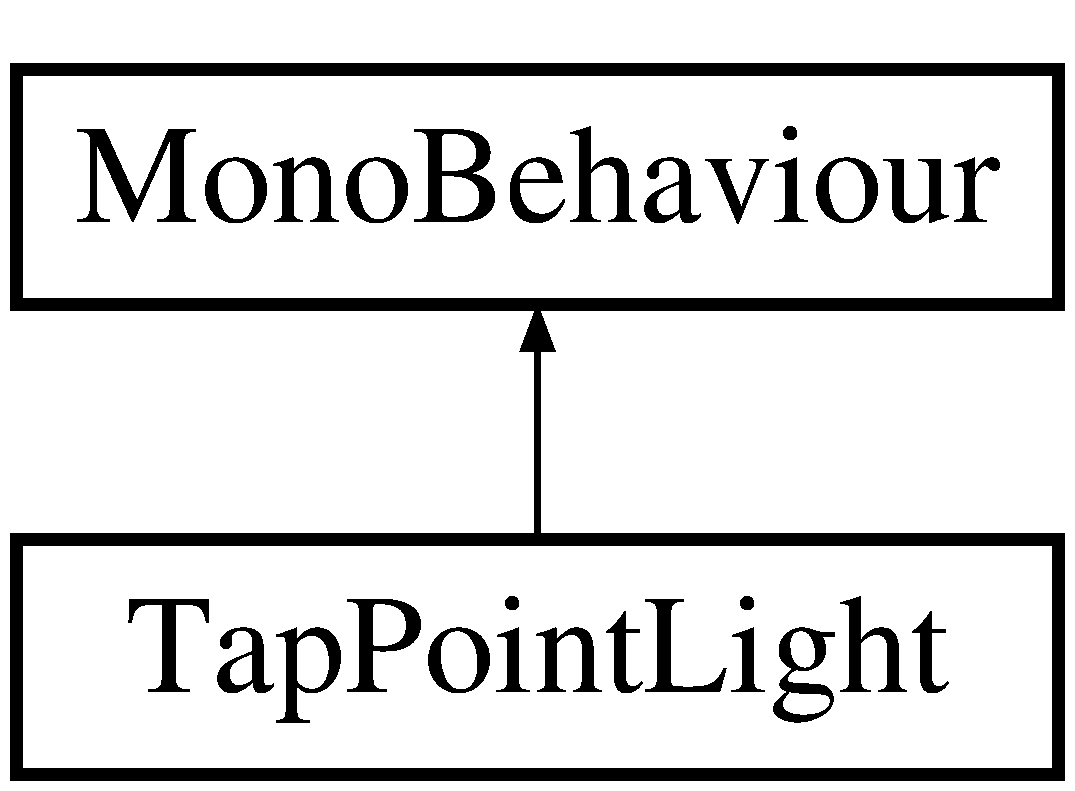
\includegraphics[height=2.000000cm]{class_tap_point_light}
\end{center}
\end{figure}
\subsection*{Public Member Functions}
\begin{DoxyCompactItemize}
\item 
void {\bfseries On\+Touch\+Down} ()\hypertarget{class_tap_point_light_a8d22c5920948cfac3451d81e9b150c90}{}\label{class_tap_point_light_a8d22c5920948cfac3451d81e9b150c90}

\end{DoxyCompactItemize}


\subsection{Detailed Description}
タップ箇所の発光 



The documentation for this class was generated from the following file\+:\begin{DoxyCompactItemize}
\item 
Scripts/\+Touch/Tap\+Point\+Light.\+cs\end{DoxyCompactItemize}

\hypertarget{class_test_scene_controller}{}\section{Test\+Scene\+Controller Class Reference}
\label{class_test_scene_controller}\index{Test\+Scene\+Controller@{Test\+Scene\+Controller}}
Inheritance diagram for Test\+Scene\+Controller\+:\begin{figure}[H]
\begin{center}
\leavevmode
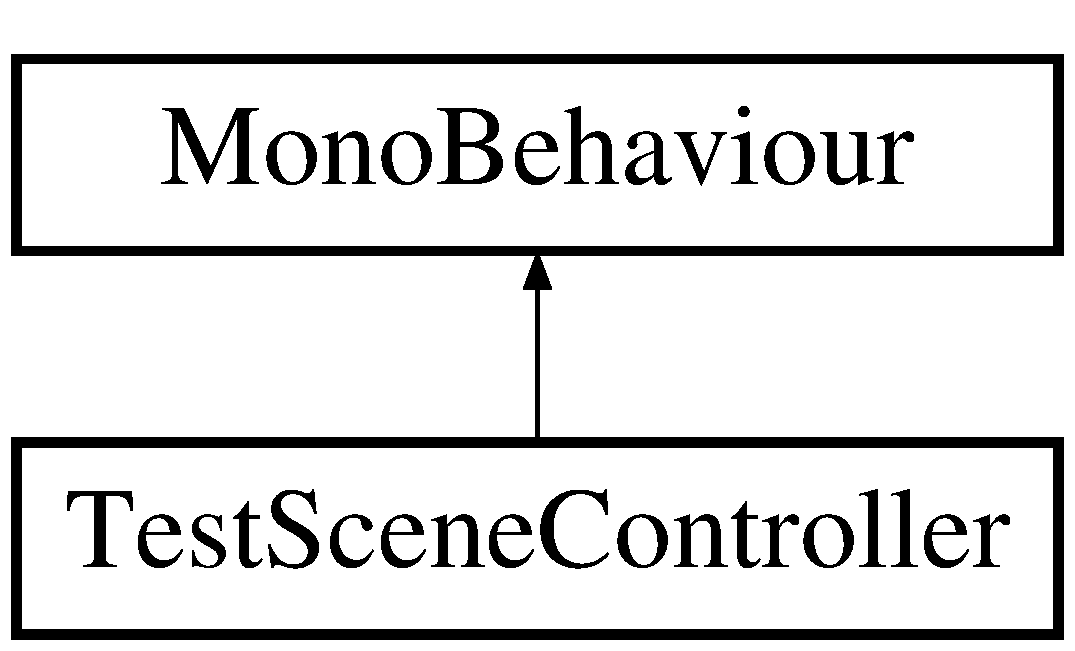
\includegraphics[height=2.000000cm]{class_test_scene_controller}
\end{center}
\end{figure}
\subsection*{Public Member Functions}
\begin{DoxyCompactItemize}
\item 
void \hyperlink{class_test_scene_controller_a17ed7e90afd9d7d339cdea394774a1bb}{Start\+Music} ()
\end{DoxyCompactItemize}
\subsection*{Public Attributes}
\begin{DoxyCompactItemize}
\item 
string {\bfseries file\+Path} = \char`\"{}/Music/0405.txt\char`\"{}\hypertarget{class_test_scene_controller_a25f3df38312529bd6581666b138f34c3}{}\label{class_test_scene_controller_a25f3df38312529bd6581666b138f34c3}

\end{DoxyCompactItemize}


\subsection{Member Function Documentation}
\index{Test\+Scene\+Controller@{Test\+Scene\+Controller}!Start\+Music@{Start\+Music}}
\index{Start\+Music@{Start\+Music}!Test\+Scene\+Controller@{Test\+Scene\+Controller}}
\subsubsection[{\texorpdfstring{Start\+Music()}{StartMusic()}}]{\setlength{\rightskip}{0pt plus 5cm}void Test\+Scene\+Controller.\+Start\+Music (
\begin{DoxyParamCaption}
{}
\end{DoxyParamCaption}
)\hspace{0.3cm}{\ttfamily [inline]}}\hypertarget{class_test_scene_controller_a17ed7e90afd9d7d339cdea394774a1bb}{}\label{class_test_scene_controller_a17ed7e90afd9d7d339cdea394774a1bb}






The documentation for this class was generated from the following file\+:\begin{DoxyCompactItemize}
\item 
Scripts/\+Scenes\+Controller/Test\+Scene\+Controller.\+cs\end{DoxyCompactItemize}

\hypertarget{class_t_m_p_text}{}\section{T\+M\+P\+Text Class Reference}
\label{class_t_m_p_text}\index{T\+M\+P\+Text@{T\+M\+P\+Text}}


T\+M\+Pテキストの拡張コンポーネント  


Inheritance diagram for T\+M\+P\+Text\+:\begin{figure}[H]
\begin{center}
\leavevmode
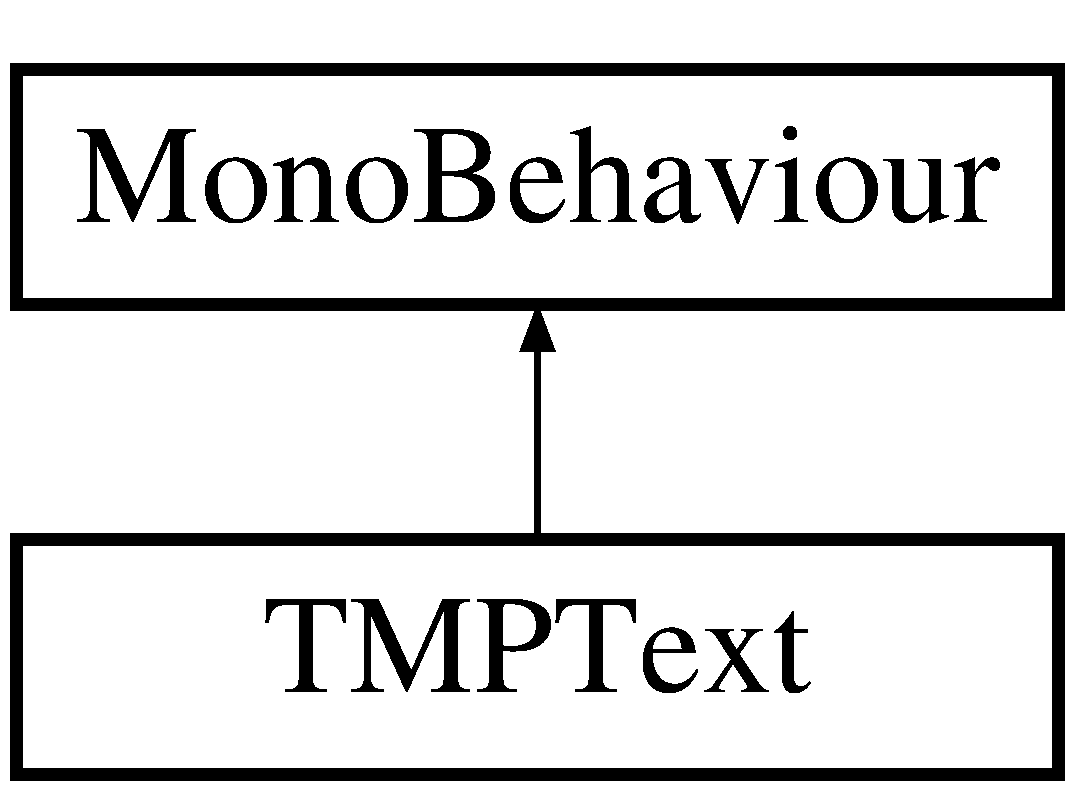
\includegraphics[height=2.000000cm]{class_t_m_p_text}
\end{center}
\end{figure}
\subsection*{Public Member Functions}
\begin{DoxyCompactItemize}
\item 
void \hyperlink{class_t_m_p_text_a2d797081623096feb8ec75c70872e8d2}{Init} ()
\begin{DoxyCompactList}\small\item\em 初期化 \end{DoxyCompactList}\item 
void \hyperlink{class_t_m_p_text_a7c1368d627b685be673316d2c41c00f6}{On\+Touch\+Up\+Color} ()
\begin{DoxyCompactList}\small\item\em 離された時の色 \end{DoxyCompactList}\item 
void \hyperlink{class_t_m_p_text_a429ef413d5ca865e547ac4ef6ca41121}{On\+Touch\+Down\+Color} ()
\begin{DoxyCompactList}\small\item\em 押された時の色 \end{DoxyCompactList}\item 
void \hyperlink{class_t_m_p_text_aafc12bdbbc7023761e6a42838375caa1}{On\+Touch\+Color} ()
\begin{DoxyCompactList}\small\item\em 押されている間の色 \end{DoxyCompactList}\item 
I\+Enumerator \hyperlink{class_t_m_p_text_a5194208ad9e965ef394335cc1c79b5e5}{Fade\+In\+Coroutine} (int fade\+Frame, System.\+Action action=null)
\begin{DoxyCompactList}\small\item\em フェードインの実装(薄くなる方) \end{DoxyCompactList}\item 
I\+Enumerator \hyperlink{class_t_m_p_text_a222dd1486fb0d17658b402c3388238e9}{Fade\+Out\+Coroutine} (int fade\+Frame, System.\+Action action=null)
\begin{DoxyCompactList}\small\item\em フェードアウトの実装(濃くなる方) \end{DoxyCompactList}\item 
I\+Enumerator {\bfseries Fade\+Loop} (float fade\+Frame)\hypertarget{class_t_m_p_text_a4239f8b3a2f164cb099892840c70d34a}{}\label{class_t_m_p_text_a4239f8b3a2f164cb099892840c70d34a}

\end{DoxyCompactItemize}
\subsection*{Properties}
\begin{DoxyCompactItemize}
\item 
Color {\bfseries Touch\+Up\+Color}\hspace{0.3cm}{\ttfamily  \mbox{[}get\mbox{]}}\hypertarget{class_t_m_p_text_ab2efc7c381fc0f998f1b97f3530ca827}{}\label{class_t_m_p_text_ab2efc7c381fc0f998f1b97f3530ca827}

\item 
Color {\bfseries Touch\+Down\+Color}\hspace{0.3cm}{\ttfamily  \mbox{[}get\mbox{]}}\hypertarget{class_t_m_p_text_a4393f4ae51df276379aeece18d81523b}{}\label{class_t_m_p_text_a4393f4ae51df276379aeece18d81523b}

\item 
Color {\bfseries Touch\+Color}\hspace{0.3cm}{\ttfamily  \mbox{[}get\mbox{]}}\hypertarget{class_t_m_p_text_a05aa418331107a0ecaa04d58f79bc5db}{}\label{class_t_m_p_text_a05aa418331107a0ecaa04d58f79bc5db}

\end{DoxyCompactItemize}


\subsection{Detailed Description}
T\+M\+Pテキストの拡張コンポーネント 



\subsection{Member Function Documentation}
\index{T\+M\+P\+Text@{T\+M\+P\+Text}!Fade\+In\+Coroutine@{Fade\+In\+Coroutine}}
\index{Fade\+In\+Coroutine@{Fade\+In\+Coroutine}!T\+M\+P\+Text@{T\+M\+P\+Text}}
\subsubsection[{\texorpdfstring{Fade\+In\+Coroutine(int fade\+Frame, System.\+Action action=null)}{FadeInCoroutine(int fadeFrame, System.Action action=null)}}]{\setlength{\rightskip}{0pt plus 5cm}I\+Enumerator T\+M\+P\+Text.\+Fade\+In\+Coroutine (
\begin{DoxyParamCaption}
\item[{int}]{fade\+Frame, }
\item[{System.\+Action}]{action = {\ttfamily null}}
\end{DoxyParamCaption}
)\hspace{0.3cm}{\ttfamily [inline]}}\hypertarget{class_t_m_p_text_a5194208ad9e965ef394335cc1c79b5e5}{}\label{class_t_m_p_text_a5194208ad9e965ef394335cc1c79b5e5}


フェードインの実装(薄くなる方) 


\begin{DoxyParams}{Parameters}
{\em fade\+Frame} & \\
\hline
\end{DoxyParams}
\begin{DoxyReturn}{Returns}

\end{DoxyReturn}
\index{T\+M\+P\+Text@{T\+M\+P\+Text}!Fade\+Out\+Coroutine@{Fade\+Out\+Coroutine}}
\index{Fade\+Out\+Coroutine@{Fade\+Out\+Coroutine}!T\+M\+P\+Text@{T\+M\+P\+Text}}
\subsubsection[{\texorpdfstring{Fade\+Out\+Coroutine(int fade\+Frame, System.\+Action action=null)}{FadeOutCoroutine(int fadeFrame, System.Action action=null)}}]{\setlength{\rightskip}{0pt plus 5cm}I\+Enumerator T\+M\+P\+Text.\+Fade\+Out\+Coroutine (
\begin{DoxyParamCaption}
\item[{int}]{fade\+Frame, }
\item[{System.\+Action}]{action = {\ttfamily null}}
\end{DoxyParamCaption}
)\hspace{0.3cm}{\ttfamily [inline]}}\hypertarget{class_t_m_p_text_a222dd1486fb0d17658b402c3388238e9}{}\label{class_t_m_p_text_a222dd1486fb0d17658b402c3388238e9}


フェードアウトの実装(濃くなる方) 


\begin{DoxyParams}{Parameters}
{\em fade\+Frame} & \\
\hline
\end{DoxyParams}
\begin{DoxyReturn}{Returns}

\end{DoxyReturn}
\index{T\+M\+P\+Text@{T\+M\+P\+Text}!Init@{Init}}
\index{Init@{Init}!T\+M\+P\+Text@{T\+M\+P\+Text}}
\subsubsection[{\texorpdfstring{Init()}{Init()}}]{\setlength{\rightskip}{0pt plus 5cm}void T\+M\+P\+Text.\+Init (
\begin{DoxyParamCaption}
{}
\end{DoxyParamCaption}
)\hspace{0.3cm}{\ttfamily [inline]}}\hypertarget{class_t_m_p_text_a2d797081623096feb8ec75c70872e8d2}{}\label{class_t_m_p_text_a2d797081623096feb8ec75c70872e8d2}


初期化 

\index{T\+M\+P\+Text@{T\+M\+P\+Text}!On\+Touch\+Color@{On\+Touch\+Color}}
\index{On\+Touch\+Color@{On\+Touch\+Color}!T\+M\+P\+Text@{T\+M\+P\+Text}}
\subsubsection[{\texorpdfstring{On\+Touch\+Color()}{OnTouchColor()}}]{\setlength{\rightskip}{0pt plus 5cm}void T\+M\+P\+Text.\+On\+Touch\+Color (
\begin{DoxyParamCaption}
{}
\end{DoxyParamCaption}
)\hspace{0.3cm}{\ttfamily [inline]}}\hypertarget{class_t_m_p_text_aafc12bdbbc7023761e6a42838375caa1}{}\label{class_t_m_p_text_aafc12bdbbc7023761e6a42838375caa1}


押されている間の色 

\index{T\+M\+P\+Text@{T\+M\+P\+Text}!On\+Touch\+Down\+Color@{On\+Touch\+Down\+Color}}
\index{On\+Touch\+Down\+Color@{On\+Touch\+Down\+Color}!T\+M\+P\+Text@{T\+M\+P\+Text}}
\subsubsection[{\texorpdfstring{On\+Touch\+Down\+Color()}{OnTouchDownColor()}}]{\setlength{\rightskip}{0pt plus 5cm}void T\+M\+P\+Text.\+On\+Touch\+Down\+Color (
\begin{DoxyParamCaption}
{}
\end{DoxyParamCaption}
)\hspace{0.3cm}{\ttfamily [inline]}}\hypertarget{class_t_m_p_text_a429ef413d5ca865e547ac4ef6ca41121}{}\label{class_t_m_p_text_a429ef413d5ca865e547ac4ef6ca41121}


押された時の色 

\index{T\+M\+P\+Text@{T\+M\+P\+Text}!On\+Touch\+Up\+Color@{On\+Touch\+Up\+Color}}
\index{On\+Touch\+Up\+Color@{On\+Touch\+Up\+Color}!T\+M\+P\+Text@{T\+M\+P\+Text}}
\subsubsection[{\texorpdfstring{On\+Touch\+Up\+Color()}{OnTouchUpColor()}}]{\setlength{\rightskip}{0pt plus 5cm}void T\+M\+P\+Text.\+On\+Touch\+Up\+Color (
\begin{DoxyParamCaption}
{}
\end{DoxyParamCaption}
)\hspace{0.3cm}{\ttfamily [inline]}}\hypertarget{class_t_m_p_text_a7c1368d627b685be673316d2c41c00f6}{}\label{class_t_m_p_text_a7c1368d627b685be673316d2c41c00f6}


離された時の色 



The documentation for this class was generated from the following file\+:\begin{DoxyCompactItemize}
\item 
Scripts/\+U\+I/T\+M\+P\+Text.\+cs\end{DoxyCompactItemize}

\hypertarget{class_touch_area_base}{}\section{Touch\+Area\+Base Class Reference}
\label{class_touch_area_base}\index{Touch\+Area\+Base@{Touch\+Area\+Base}}
Inheritance diagram for Touch\+Area\+Base\+:\begin{figure}[H]
\begin{center}
\leavevmode
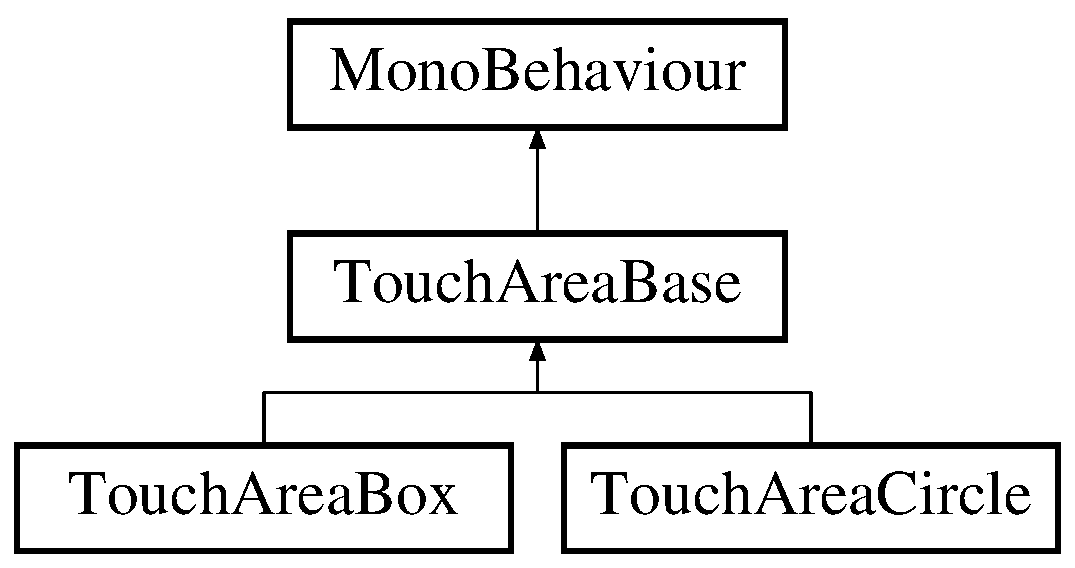
\includegraphics[height=3.000000cm]{class_touch_area_base}
\end{center}
\end{figure}
\subsection*{Public Member Functions}
\begin{DoxyCompactItemize}
\item 
\hyperlink{class_touch_area_base_a3d23db92ff531c2766cbd8547620b57d}{Touch\+Area\+Base} ()
\begin{DoxyCompactList}\small\item\em コンストラクタ \end{DoxyCompactList}\item 
void \hyperlink{class_touch_area_base_ad22019b970c42ebd4d6c9d44b5efcdcb}{Set\+Center\+Pos} (Vector3 pos)
\begin{DoxyCompactList}\small\item\em 中心点のセッター \end{DoxyCompactList}\item 
void \hyperlink{class_touch_area_base_aa63f2d3e25e2343fee2f2993a34e22ea}{Set\+Camera} (Camera camera)
\begin{DoxyCompactList}\small\item\em 座標変換に使うカメラの設定 \end{DoxyCompactList}\end{DoxyCompactItemize}
\subsection*{Protected Member Functions}
\begin{DoxyCompactItemize}
\item 
virtual void \hyperlink{class_touch_area_base_a9d4d8709065668bea45eecf59c41401b}{Set\+Transform\+Data} ()
\begin{DoxyCompactList}\small\item\em Transformの値から自身の\+Parameterを設定する \end{DoxyCompactList}\item 
virtual void \hyperlink{class_touch_area_base_a775cebdb39ddba5717a89f8ff8d1c810}{On\+Draw\+Gizmos} ()
\begin{DoxyCompactList}\small\item\em ギズモ表示 \end{DoxyCompactList}\item 
virtual void \hyperlink{class_touch_area_base_a94f9466d4f70a449055e72b86d23378c}{Reset} ()
\begin{DoxyCompactList}\small\item\em リセット時処理 \end{DoxyCompactList}\end{DoxyCompactItemize}
\subsection*{Protected Attributes}
\begin{DoxyCompactItemize}
\item 
Camera {\bfseries camera}\hypertarget{class_touch_area_base_afd86e8792674bcb666bc375f5ffbb59c}{}\label{class_touch_area_base_afd86e8792674bcb666bc375f5ffbb59c}

\item 
Vector3 {\bfseries center}\hypertarget{class_touch_area_base_aab6aa27813bea53d6965fd317ab26678}{}\label{class_touch_area_base_aab6aa27813bea53d6965fd317ab26678}

\end{DoxyCompactItemize}
\subsection*{Properties}
\begin{DoxyCompactItemize}
\item 
Vector3 {\bfseries Center}\hspace{0.3cm}{\ttfamily  \mbox{[}get\mbox{]}}\hypertarget{class_touch_area_base_aa03f7d1a17e305dbf35cf9bab9507750}{}\label{class_touch_area_base_aa03f7d1a17e305dbf35cf9bab9507750}

\item 
bool {\bfseries is\+Active}\hspace{0.3cm}{\ttfamily  \mbox{[}get, set\mbox{]}}\hypertarget{class_touch_area_base_a05cc964aef7d963af58d5f838d6057e5}{}\label{class_touch_area_base_a05cc964aef7d963af58d5f838d6057e5}

\item 
virtual bool {\bfseries is\+Touch}\hspace{0.3cm}{\ttfamily  \mbox{[}get, protected set\mbox{]}}\hypertarget{class_touch_area_base_ad08fbf97559988d8e4a4463fe0b02677}{}\label{class_touch_area_base_ad08fbf97559988d8e4a4463fe0b02677}

\end{DoxyCompactItemize}


\subsection{Constructor \& Destructor Documentation}
\index{Touch\+Area\+Base@{Touch\+Area\+Base}!Touch\+Area\+Base@{Touch\+Area\+Base}}
\index{Touch\+Area\+Base@{Touch\+Area\+Base}!Touch\+Area\+Base@{Touch\+Area\+Base}}
\subsubsection[{\texorpdfstring{Touch\+Area\+Base()}{TouchAreaBase()}}]{\setlength{\rightskip}{0pt plus 5cm}Touch\+Area\+Base.\+Touch\+Area\+Base (
\begin{DoxyParamCaption}
{}
\end{DoxyParamCaption}
)\hspace{0.3cm}{\ttfamily [inline]}}\hypertarget{class_touch_area_base_a3d23db92ff531c2766cbd8547620b57d}{}\label{class_touch_area_base_a3d23db92ff531c2766cbd8547620b57d}


コンストラクタ 



\subsection{Member Function Documentation}
\index{Touch\+Area\+Base@{Touch\+Area\+Base}!On\+Draw\+Gizmos@{On\+Draw\+Gizmos}}
\index{On\+Draw\+Gizmos@{On\+Draw\+Gizmos}!Touch\+Area\+Base@{Touch\+Area\+Base}}
\subsubsection[{\texorpdfstring{On\+Draw\+Gizmos()}{OnDrawGizmos()}}]{\setlength{\rightskip}{0pt plus 5cm}virtual void Touch\+Area\+Base.\+On\+Draw\+Gizmos (
\begin{DoxyParamCaption}
{}
\end{DoxyParamCaption}
)\hspace{0.3cm}{\ttfamily [inline]}, {\ttfamily [protected]}, {\ttfamily [virtual]}}\hypertarget{class_touch_area_base_a775cebdb39ddba5717a89f8ff8d1c810}{}\label{class_touch_area_base_a775cebdb39ddba5717a89f8ff8d1c810}


ギズモ表示 



Reimplemented in \hyperlink{class_touch_area_box_ad8e11cacc1d3089309346c13da4f2a88}{Touch\+Area\+Box}, and \hyperlink{class_touch_area_circle_a42b59d970df599ef088e0cdbc9a90329}{Touch\+Area\+Circle}.

\index{Touch\+Area\+Base@{Touch\+Area\+Base}!Reset@{Reset}}
\index{Reset@{Reset}!Touch\+Area\+Base@{Touch\+Area\+Base}}
\subsubsection[{\texorpdfstring{Reset()}{Reset()}}]{\setlength{\rightskip}{0pt plus 5cm}virtual void Touch\+Area\+Base.\+Reset (
\begin{DoxyParamCaption}
{}
\end{DoxyParamCaption}
)\hspace{0.3cm}{\ttfamily [inline]}, {\ttfamily [protected]}, {\ttfamily [virtual]}}\hypertarget{class_touch_area_base_a94f9466d4f70a449055e72b86d23378c}{}\label{class_touch_area_base_a94f9466d4f70a449055e72b86d23378c}


リセット時処理 



Reimplemented in \hyperlink{class_touch_area_box_a3ee37c987ffa5e7e23d75736e7a46483}{Touch\+Area\+Box}.

\index{Touch\+Area\+Base@{Touch\+Area\+Base}!Set\+Camera@{Set\+Camera}}
\index{Set\+Camera@{Set\+Camera}!Touch\+Area\+Base@{Touch\+Area\+Base}}
\subsubsection[{\texorpdfstring{Set\+Camera(\+Camera camera)}{SetCamera(Camera camera)}}]{\setlength{\rightskip}{0pt plus 5cm}void Touch\+Area\+Base.\+Set\+Camera (
\begin{DoxyParamCaption}
\item[{Camera}]{camera}
\end{DoxyParamCaption}
)\hspace{0.3cm}{\ttfamily [inline]}}\hypertarget{class_touch_area_base_aa63f2d3e25e2343fee2f2993a34e22ea}{}\label{class_touch_area_base_aa63f2d3e25e2343fee2f2993a34e22ea}


座標変換に使うカメラの設定 


\begin{DoxyParams}{Parameters}
{\em camera} & \\
\hline
\end{DoxyParams}
\index{Touch\+Area\+Base@{Touch\+Area\+Base}!Set\+Center\+Pos@{Set\+Center\+Pos}}
\index{Set\+Center\+Pos@{Set\+Center\+Pos}!Touch\+Area\+Base@{Touch\+Area\+Base}}
\subsubsection[{\texorpdfstring{Set\+Center\+Pos(\+Vector3 pos)}{SetCenterPos(Vector3 pos)}}]{\setlength{\rightskip}{0pt plus 5cm}void Touch\+Area\+Base.\+Set\+Center\+Pos (
\begin{DoxyParamCaption}
\item[{Vector3}]{pos}
\end{DoxyParamCaption}
)\hspace{0.3cm}{\ttfamily [inline]}}\hypertarget{class_touch_area_base_ad22019b970c42ebd4d6c9d44b5efcdcb}{}\label{class_touch_area_base_ad22019b970c42ebd4d6c9d44b5efcdcb}


中心点のセッター 


\begin{DoxyParams}{Parameters}
{\em pos} & \\
\hline
\end{DoxyParams}
\index{Touch\+Area\+Base@{Touch\+Area\+Base}!Set\+Transform\+Data@{Set\+Transform\+Data}}
\index{Set\+Transform\+Data@{Set\+Transform\+Data}!Touch\+Area\+Base@{Touch\+Area\+Base}}
\subsubsection[{\texorpdfstring{Set\+Transform\+Data()}{SetTransformData()}}]{\setlength{\rightskip}{0pt plus 5cm}virtual void Touch\+Area\+Base.\+Set\+Transform\+Data (
\begin{DoxyParamCaption}
{}
\end{DoxyParamCaption}
)\hspace{0.3cm}{\ttfamily [inline]}, {\ttfamily [protected]}, {\ttfamily [virtual]}}\hypertarget{class_touch_area_base_a9d4d8709065668bea45eecf59c41401b}{}\label{class_touch_area_base_a9d4d8709065668bea45eecf59c41401b}


Transformの値から自身の\+Parameterを設定する 



Reimplemented in \hyperlink{class_touch_area_box_a5905a11595e6007eaf06308f832cafe4}{Touch\+Area\+Box}, and \hyperlink{class_touch_area_circle_ae8c15b781f6ddee17bda483bd9c8b0a0}{Touch\+Area\+Circle}.



The documentation for this class was generated from the following file\+:\begin{DoxyCompactItemize}
\item 
Scripts/\+Touch/Touch\+Area\+Base.\+cs\end{DoxyCompactItemize}

\hypertarget{class_touch_area_box}{}\section{Touch\+Area\+Box Class Reference}
\label{class_touch_area_box}\index{Touch\+Area\+Box@{Touch\+Area\+Box}}
Inheritance diagram for Touch\+Area\+Box\+:\begin{figure}[H]
\begin{center}
\leavevmode
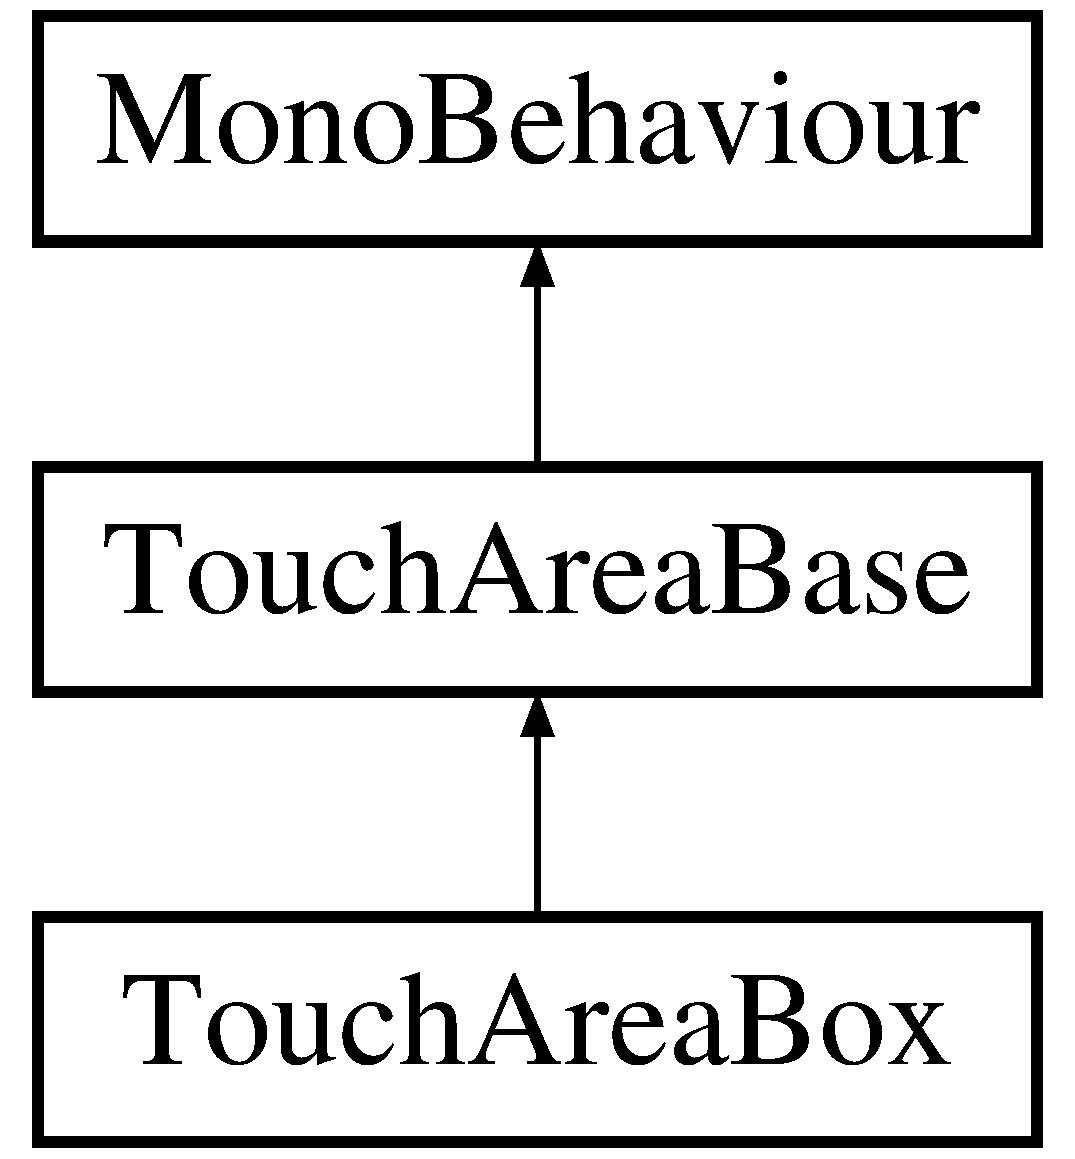
\includegraphics[height=3.000000cm]{class_touch_area_box}
\end{center}
\end{figure}
\subsection*{Public Member Functions}
\begin{DoxyCompactItemize}
\item 
void \hyperlink{class_touch_area_box_a148bf35f6965313f81ba2428e880d165}{Set\+Size} (Vector2 size)
\begin{DoxyCompactList}\small\item\em サイズのセッター \end{DoxyCompactList}\item 
void \hyperlink{class_touch_area_box_aecbf2351ec00a8848239379ddde42ce3}{Create\+Vertices} ()
\begin{DoxyCompactList}\small\item\em 矩形を構成する4頂点を生成 \end{DoxyCompactList}\item 
bool \hyperlink{class_touch_area_box_aecdfd8d0e4d80a9fb445585980386ddd}{Is\+Touch\+World\+To\+Screen} (Vector2 screen\+Pos)
\begin{DoxyCompactList}\small\item\em 当たり判定をワールド座標からスクリーン座標へ変換し、 スクリーン座標上で、この矩形と当たり判定を行う \end{DoxyCompactList}\item 
bool \hyperlink{class_touch_area_box_ab10b28047e2b6af57bac77cac9d90395}{Is\+Touch} ()
\begin{DoxyCompactList}\small\item\em タッチされているかどうか 1本でも触れていればtrueを返す \end{DoxyCompactList}\item 
bool \hyperlink{class_touch_area_box_a0fcd9e196147940919c844c0c4a1fb32}{Is\+Touch\+Began} ()
\begin{DoxyCompactList}\small\item\em タッチされた瞬間の当たり判定 1本でも存在すればtrue \end{DoxyCompactList}\item 
bool \hyperlink{class_touch_area_box_aeeb055b71f5e4cb776f2638bdebd77dd}{Is\+Touch\+End} ()
\begin{DoxyCompactList}\small\item\em タッチが離された瞬間の当たり判定 1本でも存在すればtrue \end{DoxyCompactList}\end{DoxyCompactItemize}
\subsection*{Protected Member Functions}
\begin{DoxyCompactItemize}
\item 
override void \hyperlink{class_touch_area_box_a5905a11595e6007eaf06308f832cafe4}{Set\+Transform\+Data} ()
\begin{DoxyCompactList}\small\item\em Transformの値から自身の\+Parameterを設定する \end{DoxyCompactList}\item 
override void \hyperlink{class_touch_area_box_a3ee37c987ffa5e7e23d75736e7a46483}{Reset} ()
\begin{DoxyCompactList}\small\item\em リセット時の処理 \end{DoxyCompactList}\item 
override void \hyperlink{class_touch_area_box_ad8e11cacc1d3089309346c13da4f2a88}{On\+Draw\+Gizmos} ()
\begin{DoxyCompactList}\small\item\em ギズモ表示 \end{DoxyCompactList}\end{DoxyCompactItemize}
\subsection*{Properties}
\begin{DoxyCompactItemize}
\item 
Vector2 {\bfseries Size}\hspace{0.3cm}{\ttfamily  \mbox{[}get\mbox{]}}\hypertarget{class_touch_area_box_a237928de17bd48a0e0c5c63bdf5eeb15}{}\label{class_touch_area_box_a237928de17bd48a0e0c5c63bdf5eeb15}

\item 
float {\bfseries Angle}\hspace{0.3cm}{\ttfamily  \mbox{[}get\mbox{]}}\hypertarget{class_touch_area_box_adea1cfbb523a9e251efd9fcca9392441}{}\label{class_touch_area_box_adea1cfbb523a9e251efd9fcca9392441}

\item 
override bool {\bfseries is\+Touch}\hspace{0.3cm}{\ttfamily  \mbox{[}get\mbox{]}}\hypertarget{class_touch_area_box_a883b8e1eba2bc852d71708d678cc46d3}{}\label{class_touch_area_box_a883b8e1eba2bc852d71708d678cc46d3}

\end{DoxyCompactItemize}
\subsection*{Additional Inherited Members}


\subsection{Member Function Documentation}
\index{Touch\+Area\+Box@{Touch\+Area\+Box}!Create\+Vertices@{Create\+Vertices}}
\index{Create\+Vertices@{Create\+Vertices}!Touch\+Area\+Box@{Touch\+Area\+Box}}
\subsubsection[{\texorpdfstring{Create\+Vertices()}{CreateVertices()}}]{\setlength{\rightskip}{0pt plus 5cm}void Touch\+Area\+Box.\+Create\+Vertices (
\begin{DoxyParamCaption}
{}
\end{DoxyParamCaption}
)\hspace{0.3cm}{\ttfamily [inline]}}\hypertarget{class_touch_area_box_aecbf2351ec00a8848239379ddde42ce3}{}\label{class_touch_area_box_aecbf2351ec00a8848239379ddde42ce3}


矩形を構成する4頂点を生成 

\index{Touch\+Area\+Box@{Touch\+Area\+Box}!Is\+Touch@{Is\+Touch}}
\index{Is\+Touch@{Is\+Touch}!Touch\+Area\+Box@{Touch\+Area\+Box}}
\subsubsection[{\texorpdfstring{Is\+Touch()}{IsTouch()}}]{\setlength{\rightskip}{0pt plus 5cm}bool Touch\+Area\+Box.\+Is\+Touch (
\begin{DoxyParamCaption}
{}
\end{DoxyParamCaption}
)\hspace{0.3cm}{\ttfamily [inline]}}\hypertarget{class_touch_area_box_ab10b28047e2b6af57bac77cac9d90395}{}\label{class_touch_area_box_ab10b28047e2b6af57bac77cac9d90395}


タッチされているかどうか 1本でも触れていればtrueを返す 

\begin{DoxyReturn}{Returns}

\end{DoxyReturn}
\index{Touch\+Area\+Box@{Touch\+Area\+Box}!Is\+Touch\+Began@{Is\+Touch\+Began}}
\index{Is\+Touch\+Began@{Is\+Touch\+Began}!Touch\+Area\+Box@{Touch\+Area\+Box}}
\subsubsection[{\texorpdfstring{Is\+Touch\+Began()}{IsTouchBegan()}}]{\setlength{\rightskip}{0pt plus 5cm}bool Touch\+Area\+Box.\+Is\+Touch\+Began (
\begin{DoxyParamCaption}
{}
\end{DoxyParamCaption}
)\hspace{0.3cm}{\ttfamily [inline]}}\hypertarget{class_touch_area_box_a0fcd9e196147940919c844c0c4a1fb32}{}\label{class_touch_area_box_a0fcd9e196147940919c844c0c4a1fb32}


タッチされた瞬間の当たり判定 1本でも存在すればtrue 

\begin{DoxyReturn}{Returns}

\end{DoxyReturn}
\index{Touch\+Area\+Box@{Touch\+Area\+Box}!Is\+Touch\+End@{Is\+Touch\+End}}
\index{Is\+Touch\+End@{Is\+Touch\+End}!Touch\+Area\+Box@{Touch\+Area\+Box}}
\subsubsection[{\texorpdfstring{Is\+Touch\+End()}{IsTouchEnd()}}]{\setlength{\rightskip}{0pt plus 5cm}bool Touch\+Area\+Box.\+Is\+Touch\+End (
\begin{DoxyParamCaption}
{}
\end{DoxyParamCaption}
)\hspace{0.3cm}{\ttfamily [inline]}}\hypertarget{class_touch_area_box_aeeb055b71f5e4cb776f2638bdebd77dd}{}\label{class_touch_area_box_aeeb055b71f5e4cb776f2638bdebd77dd}


タッチが離された瞬間の当たり判定 1本でも存在すればtrue 

\begin{DoxyReturn}{Returns}

\end{DoxyReturn}
\index{Touch\+Area\+Box@{Touch\+Area\+Box}!Is\+Touch\+World\+To\+Screen@{Is\+Touch\+World\+To\+Screen}}
\index{Is\+Touch\+World\+To\+Screen@{Is\+Touch\+World\+To\+Screen}!Touch\+Area\+Box@{Touch\+Area\+Box}}
\subsubsection[{\texorpdfstring{Is\+Touch\+World\+To\+Screen(\+Vector2 screen\+Pos)}{IsTouchWorldToScreen(Vector2 screenPos)}}]{\setlength{\rightskip}{0pt plus 5cm}bool Touch\+Area\+Box.\+Is\+Touch\+World\+To\+Screen (
\begin{DoxyParamCaption}
\item[{Vector2}]{screen\+Pos}
\end{DoxyParamCaption}
)\hspace{0.3cm}{\ttfamily [inline]}}\hypertarget{class_touch_area_box_aecdfd8d0e4d80a9fb445585980386ddd}{}\label{class_touch_area_box_aecdfd8d0e4d80a9fb445585980386ddd}


当たり判定をワールド座標からスクリーン座標へ変換し、 スクリーン座標上で、この矩形と当たり判定を行う 


\begin{DoxyParams}{Parameters}
{\em screen\+Pos} & \\
\hline
\end{DoxyParams}
\begin{DoxyReturn}{Returns}

\end{DoxyReturn}
\index{Touch\+Area\+Box@{Touch\+Area\+Box}!On\+Draw\+Gizmos@{On\+Draw\+Gizmos}}
\index{On\+Draw\+Gizmos@{On\+Draw\+Gizmos}!Touch\+Area\+Box@{Touch\+Area\+Box}}
\subsubsection[{\texorpdfstring{On\+Draw\+Gizmos()}{OnDrawGizmos()}}]{\setlength{\rightskip}{0pt plus 5cm}override void Touch\+Area\+Box.\+On\+Draw\+Gizmos (
\begin{DoxyParamCaption}
{}
\end{DoxyParamCaption}
)\hspace{0.3cm}{\ttfamily [inline]}, {\ttfamily [protected]}, {\ttfamily [virtual]}}\hypertarget{class_touch_area_box_ad8e11cacc1d3089309346c13da4f2a88}{}\label{class_touch_area_box_ad8e11cacc1d3089309346c13da4f2a88}


ギズモ表示 



Reimplemented from \hyperlink{class_touch_area_base_a775cebdb39ddba5717a89f8ff8d1c810}{Touch\+Area\+Base}.

\index{Touch\+Area\+Box@{Touch\+Area\+Box}!Reset@{Reset}}
\index{Reset@{Reset}!Touch\+Area\+Box@{Touch\+Area\+Box}}
\subsubsection[{\texorpdfstring{Reset()}{Reset()}}]{\setlength{\rightskip}{0pt plus 5cm}override void Touch\+Area\+Box.\+Reset (
\begin{DoxyParamCaption}
{}
\end{DoxyParamCaption}
)\hspace{0.3cm}{\ttfamily [inline]}, {\ttfamily [protected]}, {\ttfamily [virtual]}}\hypertarget{class_touch_area_box_a3ee37c987ffa5e7e23d75736e7a46483}{}\label{class_touch_area_box_a3ee37c987ffa5e7e23d75736e7a46483}


リセット時の処理 



Reimplemented from \hyperlink{class_touch_area_base_a94f9466d4f70a449055e72b86d23378c}{Touch\+Area\+Base}.

\index{Touch\+Area\+Box@{Touch\+Area\+Box}!Set\+Size@{Set\+Size}}
\index{Set\+Size@{Set\+Size}!Touch\+Area\+Box@{Touch\+Area\+Box}}
\subsubsection[{\texorpdfstring{Set\+Size(\+Vector2 size)}{SetSize(Vector2 size)}}]{\setlength{\rightskip}{0pt plus 5cm}void Touch\+Area\+Box.\+Set\+Size (
\begin{DoxyParamCaption}
\item[{Vector2}]{size}
\end{DoxyParamCaption}
)\hspace{0.3cm}{\ttfamily [inline]}}\hypertarget{class_touch_area_box_a148bf35f6965313f81ba2428e880d165}{}\label{class_touch_area_box_a148bf35f6965313f81ba2428e880d165}


サイズのセッター 


\begin{DoxyParams}{Parameters}
{\em size} & \\
\hline
\end{DoxyParams}
\index{Touch\+Area\+Box@{Touch\+Area\+Box}!Set\+Transform\+Data@{Set\+Transform\+Data}}
\index{Set\+Transform\+Data@{Set\+Transform\+Data}!Touch\+Area\+Box@{Touch\+Area\+Box}}
\subsubsection[{\texorpdfstring{Set\+Transform\+Data()}{SetTransformData()}}]{\setlength{\rightskip}{0pt plus 5cm}override void Touch\+Area\+Box.\+Set\+Transform\+Data (
\begin{DoxyParamCaption}
{}
\end{DoxyParamCaption}
)\hspace{0.3cm}{\ttfamily [inline]}, {\ttfamily [protected]}, {\ttfamily [virtual]}}\hypertarget{class_touch_area_box_a5905a11595e6007eaf06308f832cafe4}{}\label{class_touch_area_box_a5905a11595e6007eaf06308f832cafe4}


Transformの値から自身の\+Parameterを設定する 



Reimplemented from \hyperlink{class_touch_area_base_a9d4d8709065668bea45eecf59c41401b}{Touch\+Area\+Base}.



The documentation for this class was generated from the following file\+:\begin{DoxyCompactItemize}
\item 
Scripts/\+Touch/Touch\+Area\+Box.\+cs\end{DoxyCompactItemize}

\hypertarget{class_touch_area_circle}{}\section{Touch\+Area\+Circle Class Reference}
\label{class_touch_area_circle}\index{Touch\+Area\+Circle@{Touch\+Area\+Circle}}
Inheritance diagram for Touch\+Area\+Circle\+:\begin{figure}[H]
\begin{center}
\leavevmode
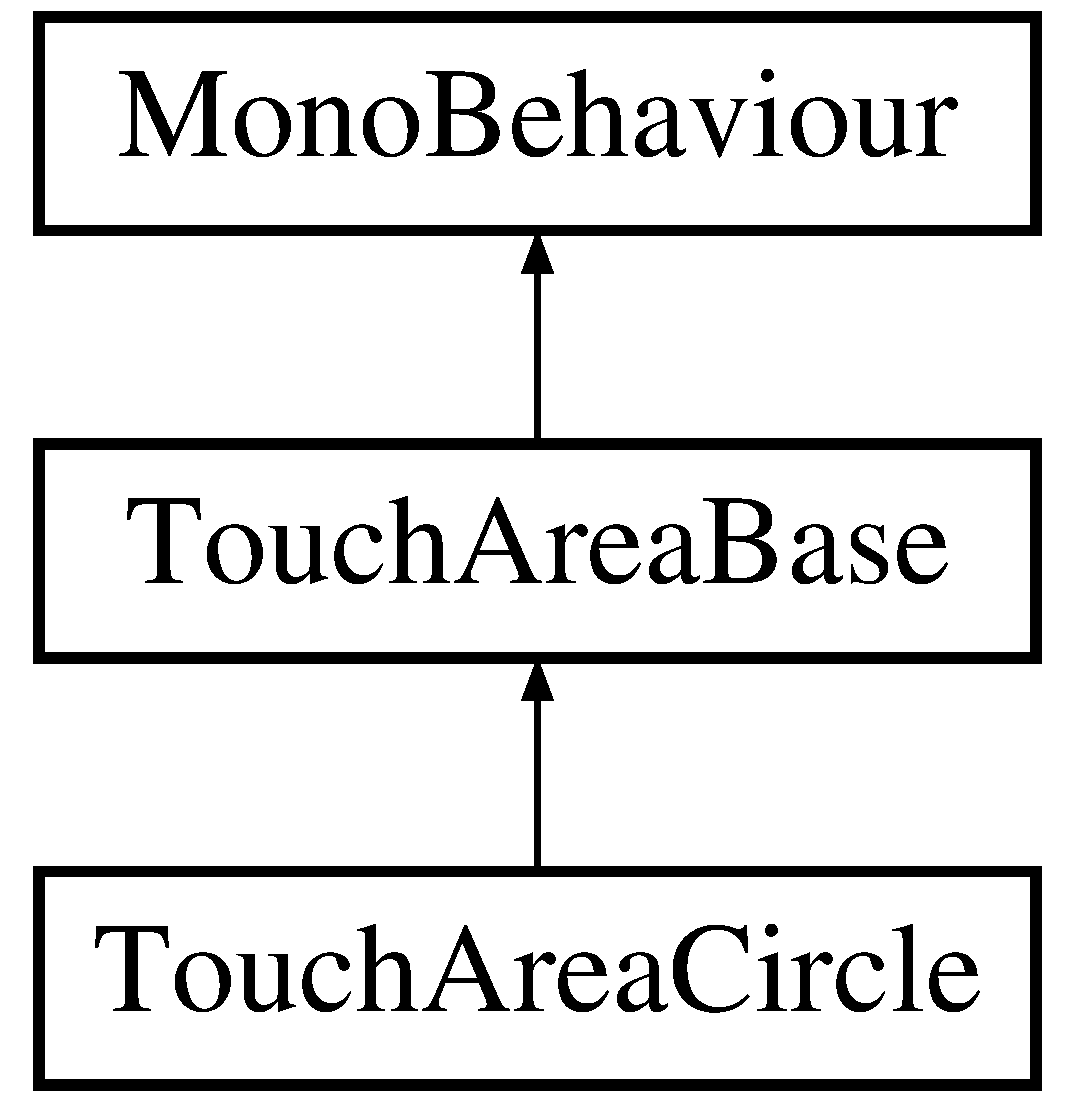
\includegraphics[height=3.000000cm]{class_touch_area_circle}
\end{center}
\end{figure}
\subsection*{Public Member Functions}
\begin{DoxyCompactItemize}
\item 
bool \hyperlink{class_touch_area_circle_a550aad828bc134613c5f207d79073073}{Is\+Touch} ()
\begin{DoxyCompactList}\small\item\em タッチされているかどうか 1本でも触れていればtrueを返す \end{DoxyCompactList}\item 
bool \hyperlink{class_touch_area_circle_afcb42f0b4356b685d22f8f12a04a61db}{Is\+Touch\+Began} ()
\begin{DoxyCompactList}\small\item\em タッチされた瞬間の当たり判定 1本でも存在すればtrue \end{DoxyCompactList}\item 
bool \hyperlink{class_touch_area_circle_adf05e73cd92075870039f9f00bc77b9b}{Is\+Touch\+End} ()
\begin{DoxyCompactList}\small\item\em 指が離された瞬間の当たり判定 1本でも存在すればtrue \end{DoxyCompactList}\end{DoxyCompactItemize}
\subsection*{Protected Member Functions}
\begin{DoxyCompactItemize}
\item 
override void \hyperlink{class_touch_area_circle_ae8c15b781f6ddee17bda483bd9c8b0a0}{Set\+Transform\+Data} ()
\begin{DoxyCompactList}\small\item\em Transformの値から自身の\+Parameterを設定する \end{DoxyCompactList}\item 
override void \hyperlink{class_touch_area_circle_a42b59d970df599ef088e0cdbc9a90329}{On\+Draw\+Gizmos} ()
\begin{DoxyCompactList}\small\item\em ギズモ表示 \end{DoxyCompactList}\end{DoxyCompactItemize}
\subsection*{Properties}
\begin{DoxyCompactItemize}
\item 
float {\bfseries Radius}\hspace{0.3cm}{\ttfamily  \mbox{[}get\mbox{]}}\hypertarget{class_touch_area_circle_ab7c2ca7c94f0670f8f5ebcf4d48c0396}{}\label{class_touch_area_circle_ab7c2ca7c94f0670f8f5ebcf4d48c0396}

\item 
override bool {\bfseries is\+Touch}\hspace{0.3cm}{\ttfamily  \mbox{[}get\mbox{]}}\hypertarget{class_touch_area_circle_aee7187303bd62a20fbe64302d3f6fff6}{}\label{class_touch_area_circle_aee7187303bd62a20fbe64302d3f6fff6}

\end{DoxyCompactItemize}
\subsection*{Additional Inherited Members}


\subsection{Member Function Documentation}
\index{Touch\+Area\+Circle@{Touch\+Area\+Circle}!Is\+Touch@{Is\+Touch}}
\index{Is\+Touch@{Is\+Touch}!Touch\+Area\+Circle@{Touch\+Area\+Circle}}
\subsubsection[{\texorpdfstring{Is\+Touch()}{IsTouch()}}]{\setlength{\rightskip}{0pt plus 5cm}bool Touch\+Area\+Circle.\+Is\+Touch (
\begin{DoxyParamCaption}
{}
\end{DoxyParamCaption}
)\hspace{0.3cm}{\ttfamily [inline]}}\hypertarget{class_touch_area_circle_a550aad828bc134613c5f207d79073073}{}\label{class_touch_area_circle_a550aad828bc134613c5f207d79073073}


タッチされているかどうか 1本でも触れていればtrueを返す 

\begin{DoxyReturn}{Returns}

\end{DoxyReturn}
\index{Touch\+Area\+Circle@{Touch\+Area\+Circle}!Is\+Touch\+Began@{Is\+Touch\+Began}}
\index{Is\+Touch\+Began@{Is\+Touch\+Began}!Touch\+Area\+Circle@{Touch\+Area\+Circle}}
\subsubsection[{\texorpdfstring{Is\+Touch\+Began()}{IsTouchBegan()}}]{\setlength{\rightskip}{0pt plus 5cm}bool Touch\+Area\+Circle.\+Is\+Touch\+Began (
\begin{DoxyParamCaption}
{}
\end{DoxyParamCaption}
)\hspace{0.3cm}{\ttfamily [inline]}}\hypertarget{class_touch_area_circle_afcb42f0b4356b685d22f8f12a04a61db}{}\label{class_touch_area_circle_afcb42f0b4356b685d22f8f12a04a61db}


タッチされた瞬間の当たり判定 1本でも存在すればtrue 

\begin{DoxyReturn}{Returns}

\end{DoxyReturn}
\index{Touch\+Area\+Circle@{Touch\+Area\+Circle}!Is\+Touch\+End@{Is\+Touch\+End}}
\index{Is\+Touch\+End@{Is\+Touch\+End}!Touch\+Area\+Circle@{Touch\+Area\+Circle}}
\subsubsection[{\texorpdfstring{Is\+Touch\+End()}{IsTouchEnd()}}]{\setlength{\rightskip}{0pt plus 5cm}bool Touch\+Area\+Circle.\+Is\+Touch\+End (
\begin{DoxyParamCaption}
{}
\end{DoxyParamCaption}
)\hspace{0.3cm}{\ttfamily [inline]}}\hypertarget{class_touch_area_circle_adf05e73cd92075870039f9f00bc77b9b}{}\label{class_touch_area_circle_adf05e73cd92075870039f9f00bc77b9b}


指が離された瞬間の当たり判定 1本でも存在すればtrue 

\begin{DoxyReturn}{Returns}

\end{DoxyReturn}
\index{Touch\+Area\+Circle@{Touch\+Area\+Circle}!On\+Draw\+Gizmos@{On\+Draw\+Gizmos}}
\index{On\+Draw\+Gizmos@{On\+Draw\+Gizmos}!Touch\+Area\+Circle@{Touch\+Area\+Circle}}
\subsubsection[{\texorpdfstring{On\+Draw\+Gizmos()}{OnDrawGizmos()}}]{\setlength{\rightskip}{0pt plus 5cm}override void Touch\+Area\+Circle.\+On\+Draw\+Gizmos (
\begin{DoxyParamCaption}
{}
\end{DoxyParamCaption}
)\hspace{0.3cm}{\ttfamily [inline]}, {\ttfamily [protected]}, {\ttfamily [virtual]}}\hypertarget{class_touch_area_circle_a42b59d970df599ef088e0cdbc9a90329}{}\label{class_touch_area_circle_a42b59d970df599ef088e0cdbc9a90329}


ギズモ表示 



Reimplemented from \hyperlink{class_touch_area_base_a775cebdb39ddba5717a89f8ff8d1c810}{Touch\+Area\+Base}.

\index{Touch\+Area\+Circle@{Touch\+Area\+Circle}!Set\+Transform\+Data@{Set\+Transform\+Data}}
\index{Set\+Transform\+Data@{Set\+Transform\+Data}!Touch\+Area\+Circle@{Touch\+Area\+Circle}}
\subsubsection[{\texorpdfstring{Set\+Transform\+Data()}{SetTransformData()}}]{\setlength{\rightskip}{0pt plus 5cm}override void Touch\+Area\+Circle.\+Set\+Transform\+Data (
\begin{DoxyParamCaption}
{}
\end{DoxyParamCaption}
)\hspace{0.3cm}{\ttfamily [inline]}, {\ttfamily [protected]}, {\ttfamily [virtual]}}\hypertarget{class_touch_area_circle_ae8c15b781f6ddee17bda483bd9c8b0a0}{}\label{class_touch_area_circle_ae8c15b781f6ddee17bda483bd9c8b0a0}


Transformの値から自身の\+Parameterを設定する 



Reimplemented from \hyperlink{class_touch_area_base_a9d4d8709065668bea45eecf59c41401b}{Touch\+Area\+Base}.



The documentation for this class was generated from the following file\+:\begin{DoxyCompactItemize}
\item 
Scripts/\+Touch/Touch\+Area\+Circle.\+cs\end{DoxyCompactItemize}

\hypertarget{class_touch_manager}{}\section{Touch\+Manager Class Reference}
\label{class_touch_manager}\index{Touch\+Manager@{Touch\+Manager}}


タッチマネージャー  


Inheritance diagram for Touch\+Manager\+:\begin{figure}[H]
\begin{center}
\leavevmode
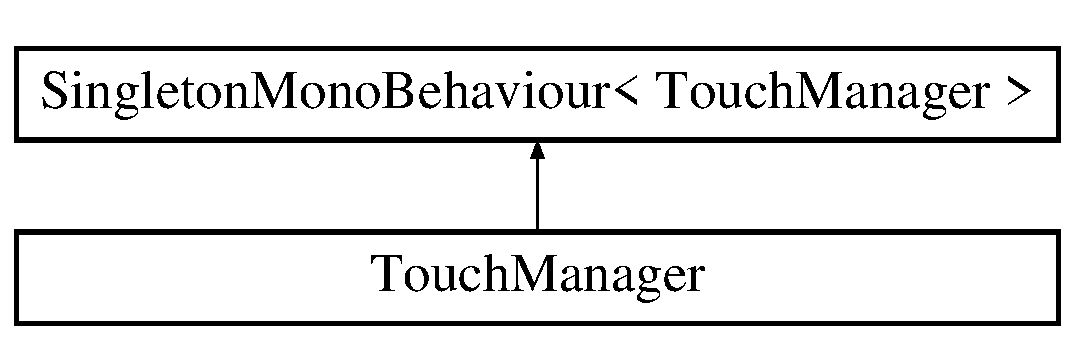
\includegraphics[height=2.000000cm]{class_touch_manager}
\end{center}
\end{figure}
\subsection*{Public Member Functions}
\begin{DoxyCompactItemize}
\item 
Vector2\mbox{[}$\,$\mbox{]} \hyperlink{class_touch_manager_a371933c19da690aa29afd51e26d3b75d}{Get\+Touch\+Pos} ()
\begin{DoxyCompactList}\small\item\em phaseに関係なくタッチされている座標を全て返す ※ Editor上ではマウスの左クリックのみ \end{DoxyCompactList}\item 
Vector2\mbox{[}$\,$\mbox{]} \hyperlink{class_touch_manager_a437d9f0a5edca24ce7d6ebea4a30ad9e}{Get\+Touch\+Began\+Pos} ()
\begin{DoxyCompactList}\small\item\em タッチした瞬間の座標を返す \end{DoxyCompactList}\item 
Vector2\mbox{[}$\,$\mbox{]} \hyperlink{class_touch_manager_af11c43ea9bc782327ad8ff5a4f151889}{Get\+Touch\+Moved\+Pos} ()
\begin{DoxyCompactList}\small\item\em 指が動かされているものの座標を返す \end{DoxyCompactList}\item 
Vector2\mbox{[}$\,$\mbox{]} \hyperlink{class_touch_manager_acdb18fa5fb6c7cc8a4ca06b3c52c53ab}{Get\+Touch\+Stationary\+Pos} ()
\begin{DoxyCompactList}\small\item\em その場でタッチされているもの(指が動かされていないもの)の座標を返す \end{DoxyCompactList}\item 
Vector2\mbox{[}$\,$\mbox{]} \hyperlink{class_touch_manager_aab5c384a916bb37c0a8c1c74f9e1b319}{Get\+Touch\+Ended\+Pos} ()
\begin{DoxyCompactList}\small\item\em 指が離れたものの座標を返す \end{DoxyCompactList}\item 
Vector2\mbox{[}$\,$\mbox{]} \hyperlink{class_touch_manager_a3cc9927c0c93ffc52e516b2322b06fb7}{Get\+Touch\+Canceled\+Pos} ()
\begin{DoxyCompactList}\small\item\em システム的に処理できないものの座標を返す ・デバイスの許容出来る指の数以上で入力された場合 ・画面買いをタップされた場合 \end{DoxyCompactList}\item 
Vector2\mbox{[}$\,$\mbox{]} \hyperlink{class_touch_manager_aaad8d2b9391c91f442cdabc9604670e8}{Get\+Touch\+Pos} (Touch\+Phase phase)
\begin{DoxyCompactList}\small\item\em phaseに該当する座標を返す \end{DoxyCompactList}\item 
bool {\bfseries Is\+Touch\+Area} (\hyperlink{class_touch_area_base}{Touch\+Area\+Base} touch\+Area)\hypertarget{class_touch_manager_aad4231928f165e0154cdc6d6fb1022a7}{}\label{class_touch_manager_aad4231928f165e0154cdc6d6fb1022a7}

\end{DoxyCompactItemize}
\subsection*{Additional Inherited Members}


\subsection{Detailed Description}
タッチマネージャー 



\subsection{Member Function Documentation}
\index{Touch\+Manager@{Touch\+Manager}!Get\+Touch\+Began\+Pos@{Get\+Touch\+Began\+Pos}}
\index{Get\+Touch\+Began\+Pos@{Get\+Touch\+Began\+Pos}!Touch\+Manager@{Touch\+Manager}}
\subsubsection[{\texorpdfstring{Get\+Touch\+Began\+Pos()}{GetTouchBeganPos()}}]{\setlength{\rightskip}{0pt plus 5cm}Vector2 \mbox{[}$\,$\mbox{]} Touch\+Manager.\+Get\+Touch\+Began\+Pos (
\begin{DoxyParamCaption}
{}
\end{DoxyParamCaption}
)\hspace{0.3cm}{\ttfamily [inline]}}\hypertarget{class_touch_manager_a437d9f0a5edca24ce7d6ebea4a30ad9e}{}\label{class_touch_manager_a437d9f0a5edca24ce7d6ebea4a30ad9e}


タッチした瞬間の座標を返す 

\begin{DoxyReturn}{Returns}

\end{DoxyReturn}
\index{Touch\+Manager@{Touch\+Manager}!Get\+Touch\+Canceled\+Pos@{Get\+Touch\+Canceled\+Pos}}
\index{Get\+Touch\+Canceled\+Pos@{Get\+Touch\+Canceled\+Pos}!Touch\+Manager@{Touch\+Manager}}
\subsubsection[{\texorpdfstring{Get\+Touch\+Canceled\+Pos()}{GetTouchCanceledPos()}}]{\setlength{\rightskip}{0pt plus 5cm}Vector2 \mbox{[}$\,$\mbox{]} Touch\+Manager.\+Get\+Touch\+Canceled\+Pos (
\begin{DoxyParamCaption}
{}
\end{DoxyParamCaption}
)\hspace{0.3cm}{\ttfamily [inline]}}\hypertarget{class_touch_manager_a3cc9927c0c93ffc52e516b2322b06fb7}{}\label{class_touch_manager_a3cc9927c0c93ffc52e516b2322b06fb7}


システム的に処理できないものの座標を返す ・デバイスの許容出来る指の数以上で入力された場合 ・画面買いをタップされた場合 

\begin{DoxyReturn}{Returns}

\end{DoxyReturn}
\index{Touch\+Manager@{Touch\+Manager}!Get\+Touch\+Ended\+Pos@{Get\+Touch\+Ended\+Pos}}
\index{Get\+Touch\+Ended\+Pos@{Get\+Touch\+Ended\+Pos}!Touch\+Manager@{Touch\+Manager}}
\subsubsection[{\texorpdfstring{Get\+Touch\+Ended\+Pos()}{GetTouchEndedPos()}}]{\setlength{\rightskip}{0pt plus 5cm}Vector2 \mbox{[}$\,$\mbox{]} Touch\+Manager.\+Get\+Touch\+Ended\+Pos (
\begin{DoxyParamCaption}
{}
\end{DoxyParamCaption}
)\hspace{0.3cm}{\ttfamily [inline]}}\hypertarget{class_touch_manager_aab5c384a916bb37c0a8c1c74f9e1b319}{}\label{class_touch_manager_aab5c384a916bb37c0a8c1c74f9e1b319}


指が離れたものの座標を返す 

\begin{DoxyReturn}{Returns}

\end{DoxyReturn}
\index{Touch\+Manager@{Touch\+Manager}!Get\+Touch\+Moved\+Pos@{Get\+Touch\+Moved\+Pos}}
\index{Get\+Touch\+Moved\+Pos@{Get\+Touch\+Moved\+Pos}!Touch\+Manager@{Touch\+Manager}}
\subsubsection[{\texorpdfstring{Get\+Touch\+Moved\+Pos()}{GetTouchMovedPos()}}]{\setlength{\rightskip}{0pt plus 5cm}Vector2 \mbox{[}$\,$\mbox{]} Touch\+Manager.\+Get\+Touch\+Moved\+Pos (
\begin{DoxyParamCaption}
{}
\end{DoxyParamCaption}
)\hspace{0.3cm}{\ttfamily [inline]}}\hypertarget{class_touch_manager_af11c43ea9bc782327ad8ff5a4f151889}{}\label{class_touch_manager_af11c43ea9bc782327ad8ff5a4f151889}


指が動かされているものの座標を返す 

\begin{DoxyReturn}{Returns}

\end{DoxyReturn}
\index{Touch\+Manager@{Touch\+Manager}!Get\+Touch\+Pos@{Get\+Touch\+Pos}}
\index{Get\+Touch\+Pos@{Get\+Touch\+Pos}!Touch\+Manager@{Touch\+Manager}}
\subsubsection[{\texorpdfstring{Get\+Touch\+Pos()}{GetTouchPos()}}]{\setlength{\rightskip}{0pt plus 5cm}Vector2 \mbox{[}$\,$\mbox{]} Touch\+Manager.\+Get\+Touch\+Pos (
\begin{DoxyParamCaption}
{}
\end{DoxyParamCaption}
)\hspace{0.3cm}{\ttfamily [inline]}}\hypertarget{class_touch_manager_a371933c19da690aa29afd51e26d3b75d}{}\label{class_touch_manager_a371933c19da690aa29afd51e26d3b75d}


phaseに関係なくタッチされている座標を全て返す ※ Editor上ではマウスの左クリックのみ 

\begin{DoxyReturn}{Returns}

\end{DoxyReturn}
\index{Touch\+Manager@{Touch\+Manager}!Get\+Touch\+Pos@{Get\+Touch\+Pos}}
\index{Get\+Touch\+Pos@{Get\+Touch\+Pos}!Touch\+Manager@{Touch\+Manager}}
\subsubsection[{\texorpdfstring{Get\+Touch\+Pos(\+Touch\+Phase phase)}{GetTouchPos(TouchPhase phase)}}]{\setlength{\rightskip}{0pt plus 5cm}Vector2 \mbox{[}$\,$\mbox{]} Touch\+Manager.\+Get\+Touch\+Pos (
\begin{DoxyParamCaption}
\item[{Touch\+Phase}]{phase}
\end{DoxyParamCaption}
)\hspace{0.3cm}{\ttfamily [inline]}}\hypertarget{class_touch_manager_aaad8d2b9391c91f442cdabc9604670e8}{}\label{class_touch_manager_aaad8d2b9391c91f442cdabc9604670e8}


phaseに該当する座標を返す 


\begin{DoxyParams}{Parameters}
{\em phase} & \\
\hline
\end{DoxyParams}
\begin{DoxyReturn}{Returns}

\end{DoxyReturn}
\index{Touch\+Manager@{Touch\+Manager}!Get\+Touch\+Stationary\+Pos@{Get\+Touch\+Stationary\+Pos}}
\index{Get\+Touch\+Stationary\+Pos@{Get\+Touch\+Stationary\+Pos}!Touch\+Manager@{Touch\+Manager}}
\subsubsection[{\texorpdfstring{Get\+Touch\+Stationary\+Pos()}{GetTouchStationaryPos()}}]{\setlength{\rightskip}{0pt plus 5cm}Vector2 \mbox{[}$\,$\mbox{]} Touch\+Manager.\+Get\+Touch\+Stationary\+Pos (
\begin{DoxyParamCaption}
{}
\end{DoxyParamCaption}
)\hspace{0.3cm}{\ttfamily [inline]}}\hypertarget{class_touch_manager_acdb18fa5fb6c7cc8a4ca06b3c52c53ab}{}\label{class_touch_manager_acdb18fa5fb6c7cc8a4ca06b3c52c53ab}


その場でタッチされているもの(指が動かされていないもの)の座標を返す 

\begin{DoxyReturn}{Returns}

\end{DoxyReturn}


The documentation for this class was generated from the following file\+:\begin{DoxyCompactItemize}
\item 
Scripts/\+Touch/Touch\+Manager.\+cs\end{DoxyCompactItemize}

\hypertarget{class_u_i_image}{}\section{U\+I\+Image Class Reference}
\label{class_u_i_image}\index{U\+I\+Image@{U\+I\+Image}}
Inheritance diagram for U\+I\+Image\+:\begin{figure}[H]
\begin{center}
\leavevmode
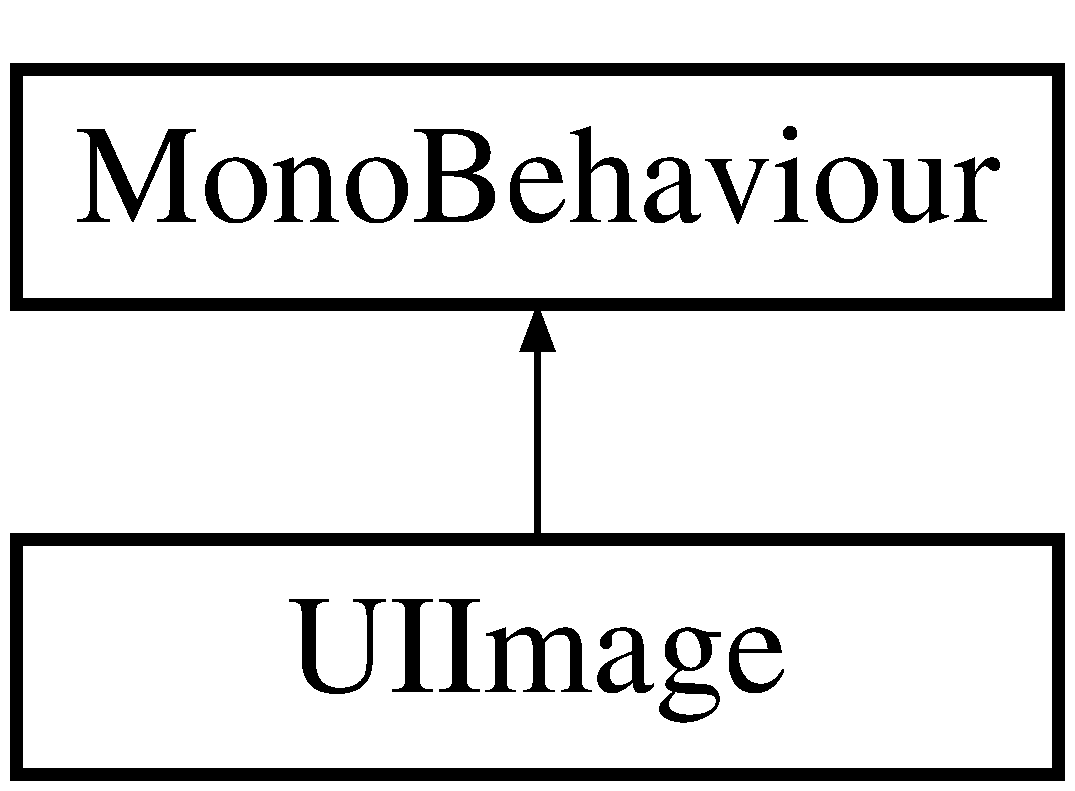
\includegraphics[height=2.000000cm]{class_u_i_image}
\end{center}
\end{figure}
\subsection*{Public Member Functions}
\begin{DoxyCompactItemize}
\item 
void \hyperlink{class_u_i_image_a88eef4b3643e666976c81aa36aa1c943}{Init} ()
\begin{DoxyCompactList}\small\item\em 初期化 \end{DoxyCompactList}\item 
void \hyperlink{class_u_i_image_af72aac7a3a2ab82901302332cf8f9eb4}{On\+Touch\+Up\+Color} ()
\begin{DoxyCompactList}\small\item\em 離された時の色 \end{DoxyCompactList}\item 
void \hyperlink{class_u_i_image_aa51089a52c0b9f9776b5af8ac2704603}{On\+Touch\+Down\+Color} ()
\begin{DoxyCompactList}\small\item\em 押された時の色 \end{DoxyCompactList}\item 
void \hyperlink{class_u_i_image_aa6038f3fb4dc283e367936f1c8f71558}{On\+Touch\+Color} ()
\begin{DoxyCompactList}\small\item\em 押されている間の色 \end{DoxyCompactList}\end{DoxyCompactItemize}
\subsection*{Properties}
\begin{DoxyCompactItemize}
\item 
Color {\bfseries Touch\+Up\+Color}\hspace{0.3cm}{\ttfamily  \mbox{[}get\mbox{]}}\hypertarget{class_u_i_image_afa850769ecd749111c6d564f04d4935d}{}\label{class_u_i_image_afa850769ecd749111c6d564f04d4935d}

\item 
Color {\bfseries Touch\+Down\+Color}\hspace{0.3cm}{\ttfamily  \mbox{[}get\mbox{]}}\hypertarget{class_u_i_image_ab39fdbfd72c4d5d2ecca63298d43a77a}{}\label{class_u_i_image_ab39fdbfd72c4d5d2ecca63298d43a77a}

\item 
Color {\bfseries Touch\+Color}\hspace{0.3cm}{\ttfamily  \mbox{[}get\mbox{]}}\hypertarget{class_u_i_image_aef098e04c6379f76f8bf32974cf9eecb}{}\label{class_u_i_image_aef098e04c6379f76f8bf32974cf9eecb}

\end{DoxyCompactItemize}


\subsection{Member Function Documentation}
\index{U\+I\+Image@{U\+I\+Image}!Init@{Init}}
\index{Init@{Init}!U\+I\+Image@{U\+I\+Image}}
\subsubsection[{\texorpdfstring{Init()}{Init()}}]{\setlength{\rightskip}{0pt plus 5cm}void U\+I\+Image.\+Init (
\begin{DoxyParamCaption}
{}
\end{DoxyParamCaption}
)\hspace{0.3cm}{\ttfamily [inline]}}\hypertarget{class_u_i_image_a88eef4b3643e666976c81aa36aa1c943}{}\label{class_u_i_image_a88eef4b3643e666976c81aa36aa1c943}


初期化 

\index{U\+I\+Image@{U\+I\+Image}!On\+Touch\+Color@{On\+Touch\+Color}}
\index{On\+Touch\+Color@{On\+Touch\+Color}!U\+I\+Image@{U\+I\+Image}}
\subsubsection[{\texorpdfstring{On\+Touch\+Color()}{OnTouchColor()}}]{\setlength{\rightskip}{0pt plus 5cm}void U\+I\+Image.\+On\+Touch\+Color (
\begin{DoxyParamCaption}
{}
\end{DoxyParamCaption}
)\hspace{0.3cm}{\ttfamily [inline]}}\hypertarget{class_u_i_image_aa6038f3fb4dc283e367936f1c8f71558}{}\label{class_u_i_image_aa6038f3fb4dc283e367936f1c8f71558}


押されている間の色 

\index{U\+I\+Image@{U\+I\+Image}!On\+Touch\+Down\+Color@{On\+Touch\+Down\+Color}}
\index{On\+Touch\+Down\+Color@{On\+Touch\+Down\+Color}!U\+I\+Image@{U\+I\+Image}}
\subsubsection[{\texorpdfstring{On\+Touch\+Down\+Color()}{OnTouchDownColor()}}]{\setlength{\rightskip}{0pt plus 5cm}void U\+I\+Image.\+On\+Touch\+Down\+Color (
\begin{DoxyParamCaption}
{}
\end{DoxyParamCaption}
)\hspace{0.3cm}{\ttfamily [inline]}}\hypertarget{class_u_i_image_aa51089a52c0b9f9776b5af8ac2704603}{}\label{class_u_i_image_aa51089a52c0b9f9776b5af8ac2704603}


押された時の色 

\index{U\+I\+Image@{U\+I\+Image}!On\+Touch\+Up\+Color@{On\+Touch\+Up\+Color}}
\index{On\+Touch\+Up\+Color@{On\+Touch\+Up\+Color}!U\+I\+Image@{U\+I\+Image}}
\subsubsection[{\texorpdfstring{On\+Touch\+Up\+Color()}{OnTouchUpColor()}}]{\setlength{\rightskip}{0pt plus 5cm}void U\+I\+Image.\+On\+Touch\+Up\+Color (
\begin{DoxyParamCaption}
{}
\end{DoxyParamCaption}
)\hspace{0.3cm}{\ttfamily [inline]}}\hypertarget{class_u_i_image_af72aac7a3a2ab82901302332cf8f9eb4}{}\label{class_u_i_image_af72aac7a3a2ab82901302332cf8f9eb4}


離された時の色 



The documentation for this class was generated from the following file\+:\begin{DoxyCompactItemize}
\item 
Scripts/\+U\+I/U\+I\+Image.\+cs\end{DoxyCompactItemize}

\hypertarget{class_viewers_controller}{}\section{Viewers\+Controller Class Reference}
\label{class_viewers_controller}\index{Viewers\+Controller@{Viewers\+Controller}}
Inheritance diagram for Viewers\+Controller\+:\begin{figure}[H]
\begin{center}
\leavevmode
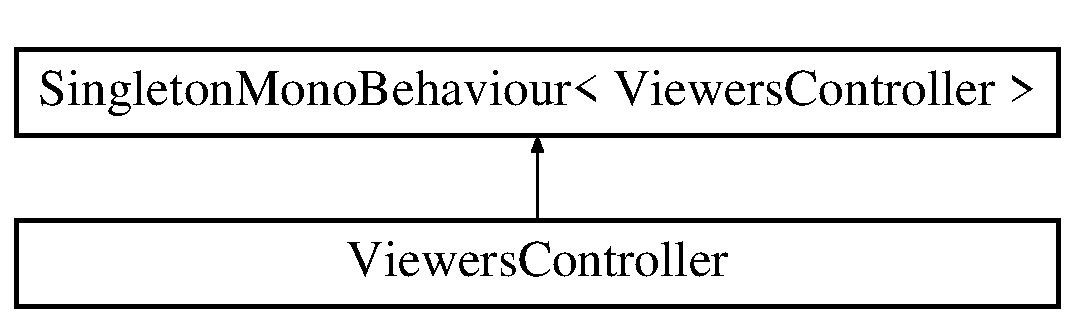
\includegraphics[height=2.000000cm]{class_viewers_controller}
\end{center}
\end{figure}
\subsection*{Public Member Functions}
\begin{DoxyCompactItemize}
\item 
void {\bfseries End\+Move} ()\hypertarget{class_viewers_controller_a958c6ef12757f0efd9f1afb44b7ab696}{}\label{class_viewers_controller_a958c6ef12757f0efd9f1afb44b7ab696}

\item 
void {\bfseries Pause} ()\hypertarget{class_viewers_controller_a36ae39a64f0006f7e58cbce843ddc7e6}{}\label{class_viewers_controller_a36ae39a64f0006f7e58cbce843ddc7e6}

\item 
void {\bfseries Un\+Pause} ()\hypertarget{class_viewers_controller_aaf983938c60c79c987f19ee40cab94b2}{}\label{class_viewers_controller_aaf983938c60c79c987f19ee40cab94b2}

\item 
void \hyperlink{class_viewers_controller_a9fb0ed2747358b5ece64b300589e3bdd}{update} ()
\begin{DoxyCompactList}\small\item\em コンボ数に応じて盛り上がりを変化させる ※テンションが変わるときのみ入るように注意! \end{DoxyCompactList}\item 
int \hyperlink{class_viewers_controller_a137bc9b08416e19972912dd5be3329f8}{Convert\+Tension\+Code} (int combo)
\begin{DoxyCompactList}\small\item\em 引数のコンボ数の時のテンションコードを返す テンションコードとはテンションの種類に応じた値である \end{DoxyCompactList}\end{DoxyCompactItemize}
\subsection*{Additional Inherited Members}


\subsection{Member Function Documentation}
\index{Viewers\+Controller@{Viewers\+Controller}!Convert\+Tension\+Code@{Convert\+Tension\+Code}}
\index{Convert\+Tension\+Code@{Convert\+Tension\+Code}!Viewers\+Controller@{Viewers\+Controller}}
\subsubsection[{\texorpdfstring{Convert\+Tension\+Code(int combo)}{ConvertTensionCode(int combo)}}]{\setlength{\rightskip}{0pt plus 5cm}int Viewers\+Controller.\+Convert\+Tension\+Code (
\begin{DoxyParamCaption}
\item[{int}]{combo}
\end{DoxyParamCaption}
)\hspace{0.3cm}{\ttfamily [inline]}}\hypertarget{class_viewers_controller_a137bc9b08416e19972912dd5be3329f8}{}\label{class_viewers_controller_a137bc9b08416e19972912dd5be3329f8}


引数のコンボ数の時のテンションコードを返す テンションコードとはテンションの種類に応じた値である 


\begin{DoxyParams}{Parameters}
{\em combo} & \\
\hline
\end{DoxyParams}
\begin{DoxyReturn}{Returns}

\end{DoxyReturn}
\index{Viewers\+Controller@{Viewers\+Controller}!update@{update}}
\index{update@{update}!Viewers\+Controller@{Viewers\+Controller}}
\subsubsection[{\texorpdfstring{update()}{update()}}]{\setlength{\rightskip}{0pt plus 5cm}void Viewers\+Controller.\+update (
\begin{DoxyParamCaption}
{}
\end{DoxyParamCaption}
)\hspace{0.3cm}{\ttfamily [inline]}}\hypertarget{class_viewers_controller_a9fb0ed2747358b5ece64b300589e3bdd}{}\label{class_viewers_controller_a9fb0ed2747358b5ece64b300589e3bdd}


コンボ数に応じて盛り上がりを変化させる ※テンションが変わるときのみ入るように注意! 



The documentation for this class was generated from the following file\+:\begin{DoxyCompactItemize}
\item 
Scripts/\+Viewers/Viewers\+Controller.\+cs\end{DoxyCompactItemize}

\hypertarget{class_wave_t_m_p_text}{}\section{Wave\+T\+M\+P\+Text Class Reference}
\label{class_wave_t_m_p_text}\index{Wave\+T\+M\+P\+Text@{Wave\+T\+M\+P\+Text}}


T\+M\+P\+Textのウェーブ  


Inheritance diagram for Wave\+T\+M\+P\+Text\+:\begin{figure}[H]
\begin{center}
\leavevmode
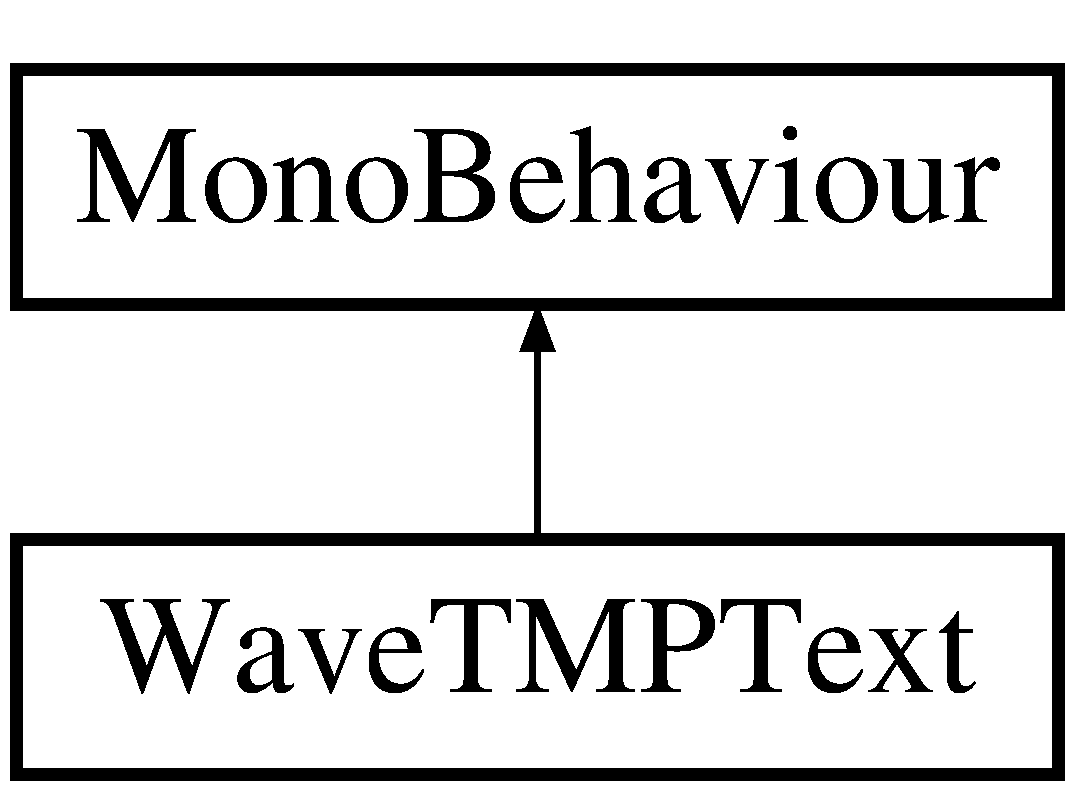
\includegraphics[height=2.000000cm]{class_wave_t_m_p_text}
\end{center}
\end{figure}


\subsection{Detailed Description}
T\+M\+P\+Textのウェーブ 



The documentation for this class was generated from the following file\+:\begin{DoxyCompactItemize}
\item 
Scripts/\+U\+I/Wave\+T\+M\+P\+Text.\+cs\end{DoxyCompactItemize}

%--- End generated contents ---

% Index
\backmatter
\newpage
\phantomsection
\clearemptydoublepage
\addcontentsline{toc}{chapter}{Index}
\printindex

\end{document}
